% Version 1.0 January 2009
%
% To compile to pdf, run:
% latex plos.template
% bibtex plos.template
% latex plos.template
% latex plos.template
% dvipdf plos.template

\documentclass[10pt]{article}\usepackage[]{graphicx}\usepackage[]{color}
%% maxwidth is the original width if it is less than linewidth
%% otherwise use linewidth (to make sure the graphics do not exceed the margin)
\makeatletter
\def\maxwidth{ %
  \ifdim\Gin@nat@width>\linewidth
    \linewidth
  \else
    \Gin@nat@width
  \fi
}
\makeatother

\definecolor{fgcolor}{rgb}{0.345, 0.345, 0.345}
\newcommand{\hlnum}[1]{\textcolor[rgb]{0.686,0.059,0.569}{#1}}%
\newcommand{\hlstr}[1]{\textcolor[rgb]{0.192,0.494,0.8}{#1}}%
\newcommand{\hlcom}[1]{\textcolor[rgb]{0.678,0.584,0.686}{\textit{#1}}}%
\newcommand{\hlopt}[1]{\textcolor[rgb]{0,0,0}{#1}}%
\newcommand{\hlstd}[1]{\textcolor[rgb]{0.345,0.345,0.345}{#1}}%
\newcommand{\hlkwa}[1]{\textcolor[rgb]{0.161,0.373,0.58}{\textbf{#1}}}%
\newcommand{\hlkwb}[1]{\textcolor[rgb]{0.69,0.353,0.396}{#1}}%
\newcommand{\hlkwc}[1]{\textcolor[rgb]{0.333,0.667,0.333}{#1}}%
\newcommand{\hlkwd}[1]{\textcolor[rgb]{0.737,0.353,0.396}{\textbf{#1}}}%

\usepackage{framed}
\makeatletter
\newenvironment{kframe}{%
 \def\at@end@of@kframe{}%
 \ifinner\ifhmode%
  \def\at@end@of@kframe{\end{minipage}}%
  \begin{minipage}{\columnwidth}%
 \fi\fi%
 \def\FrameCommand##1{\hskip\@totalleftmargin \hskip-\fboxsep
 \colorbox{shadecolor}{##1}\hskip-\fboxsep
     % There is no \\@totalrightmargin, so:
     \hskip-\linewidth \hskip-\@totalleftmargin \hskip\columnwidth}%
 \MakeFramed {\advance\hsize-\width
   \@totalleftmargin\z@ \linewidth\hsize
   \@setminipage}}%
 {\par\unskip\endMakeFramed%
 \at@end@of@kframe}
\makeatother

\definecolor{shadecolor}{rgb}{.97, .97, .97}
\definecolor{messagecolor}{rgb}{0, 0, 0}
\definecolor{warningcolor}{rgb}{1, 0, 1}
\definecolor{errorcolor}{rgb}{1, 0, 0}
\newenvironment{knitrout}{}{} % an empty environment to be redefined in TeX

\usepackage{alltt}

\usepackage{amsmath, amssymb, graphicx, color, enumerate, float}

% Use doublespacing - comment out for single spacing
%\usepackage{setspace} 
%\doublespacing

% Text layout
\topmargin 0.0cm
\oddsidemargin 0.5cm
\evensidemargin 0.5cm
\textwidth 16cm 
\textheight 21cm

\usepackage{ifxetex}
\ifxetex
%\usepackage{fontspec}
  \usepackage{unicode-math}
  \setmathfont{[Asana-Math]}
\fi

\usepackage[
  natbib = true,
    backend=bibtex,
    isbn=false,
    url=false,
    doi=false,
    eprint=false,
    style=numeric,
    sorting=nyt,
    sortcites = true
]{biblatex}
\bibliography{CT_Pipeline_l}


% Bold the 'Figure #' in the caption and separate it with a period
% Captions will be left justified
\usepackage[labelfont=bf,labelsep=period,justification=raggedright,tableposition=bottom]{caption}

% Use the PLoS provided bibtex style

% Remove brackets from numbering in List of References
\newcommand{\bbeta}{\mbox{\boldmath $\beta$}}

% Leave date blank
\date{}
\pagestyle{myheadings}
% \usepackage{natbib}
\usepackage{subfig}
\usepackage{hyperref}
\graphicspath{{maps/}}
\IfFileExists{upquote.sty}{\usepackage{upquote}}{}
\begin{document}

\begin{flushleft}
{\Large
\textbf{Intracranial Hemorrhage Localization in a Population of Patients using Registration-based Techniques in CT Imaging}
}
\\
John Muschelli$^{1,\ast}$,  
Natalie L. Ullman$^{2}$,
Elizabeth M. Sweeney$^{3}$,
Ani Eloyan$^{4}$,
Daniel F. Hanley$^{5}$,
Ciprian M. Crainiceanu$^{6}$
\\
\bf{1} John Muschelli Department of Biostatistics, Bloomberg School of Public Health, Johns Hopkins University, Baltimore, MD, USA
\\
\bf{2} Natalie L. Ullman Department of Neurology, Division of Brain Injury Outcomes,  Johns Hopkins Medical Institutions, Baltimore, MD, USA
\\
\bf{3} Elizabeth M. Sweeney, Department of Biostatistics, Bloomberg School of Public Health, Johns Hopkins University, Baltimore, MD, USA
\\
\bf{4} Ani Eloyan, Department of Biostatistics, Bloomberg School of Public Health, Johns Hopkins University, Baltimore, MD, USA
\\
\bf{5} Daniel F. Hanley Department of Neurology, Division of Brain Injury Outcomes,  Johns Hopkins Medical Institutions, Baltimore, MD, USA
\\
\bf{6} Ciprian M. Crainiceanu Department of Biostatistics, Bloomberg School of Public Health, Johns Hopkins University, Baltimore, MD, USA
\\
$\ast$ E-mail: Corresponding jmusche1@jhu.edu
\end{flushleft}


% Please keep the abstract between 250 and 300 words
\section*{Abstract}

NA

{\bf Keywords:} Intracranial Hemorrhage; CT Imaging Analysis; 3D Histograms;










\section{Introduction}

Intracranial hemorrhage (ICH) is a neurological condition that results from a blood vessel rupturing into tissues and possibly the ventricles of the brain.  Bleeding may cause distension of the brain structures and increase in potentially lethal intracranial pressure (ICP).  ICH is a serious condition; it accounts for approximately 10-15\% of all strokes, corresponding to an estimated 79,500 annual cases \citep{go_heart_2013} and approximately 30,000 deaths \citep{qureshi_spontaneous_2001} in the US and approximately 5 million cases worldwide \citep{krishnamurthi_global_2014}. In addition to the increased likelihood of death, ICH has debilitating health effects on survivors who do not have full functional recovery after stroke.

The use of computed tomography (CT) scans allows clinicians and researchers to qualitatively and quantitatively describe the characteristics of a hemorrhage to guide interventions and treatments.  CT scanning is widely available and is the most commonly used diagnostic tool in patients with ICH \citep{sahni_management_2007}. While much can be understood from careful CT image inspection, detailed quantification of information at the patient and population level is an open problem. Indeed, it is hard, for example, to quantify from visual inspection alone the percent of a particular anatomic region of interest (ROI) engaged by the stroke, compare locations of strokes across patients, and study the association between specific locations and adverse health outcomes.

To address these problems, we will 1) develop an analytic pipeline based on available neuroimaging tools to register patient CT scans to a CT template; 2) create a 3-dimensional (3D) density map of hemorrhages occurring in a population of patients who survived initial ICH and were enrolled in the MISTIE and ICES clinical trials; 3) provide a detailed quantification of hemorrhage engagement of individual neuroanatomic regions within the brain; 4) determine if differences in location relate to two common disability scores: the National Institutes of Health Stroke Scale (NIHSS) \citep{brott_measurements_1989} 
and the modified Glasgow Coma Scale (GCS) \citep{teasdale_assessment_1974, teasdale_assessment_1976}; 
and 5) generate a stroke region of engagement that is likely to be associated with adverse health effects and test its predictive performance using within-sample validation.

It is a matter of debate whether the location of the ICH is relevant to functional outcome in patients who survived to make it to the hospital \citep{carhuapoma_intracerebral_2009}. For example, \citet{hemphill_ich_2001} found that infratentorial ICH location, intraventricular involvement, and ICH volume, which may represent a number of anatomic locations, all predict 30-day mortality. Conversely, \citet{chuang_risk_2009}, and \citet{diringer_hydrocephalus:_1998} found that the site of ICH was associated with 30-day mortality, but was not statistically associated after adjusting for other covariates.  Following the result that hydrocephalus was an independent predictor of 30-day mortality \citep{diringer_hydrocephalus:_1998}, \citet{phan_hydrocephalus_2000} found that hydrocephalus was an independent prognostic indicator only for the group with hemorrhages in the putamen and not for those with hemorrhages in the caudate or thalamus. In contrast, other studies have not observed location of the ICH predicting prognosis \citep{portenoy_intracerebral_1987, senant_[multi-factorial_1988, daverat_death_1991, broderick_volume_1993, lisk_early_1994, mase_immediate_1995, qureshi_predictors_1995, razzaq_determinants_1998, hallevy_spontaneous_2002, cheung_use_2003}.  

Other trials have estimated the effects of surgery in a sub-population of ICH patients on health outcomes. % , but little continues to be known about the association between stroke localization and health outcomes among initial stroke survivors. 
Phase I of the Surgical Trial in Intracerebral Haemorrhage (STICH I) found treatment effects of hemorrhage reduction through early surgery in a subset of patients who had bleeds in the proximity of the brain lobes ($\leq$1 cm from the cortical surface of the brain) \citep{mendelow_early_2005}. However, when the effect was re-examined in the second phase of the trial (STICH II), which included only patients with superficial lobar hematomas, the treatment effect was not found to be statistically significant \citep{mendelow_early_2013}.  Although STICH II did not identify a statistically significant treatment effect, this may be due to sub-optimal definition of localization.  In the ``Guidelines for the Management of Spontaneous Intracerebral Hemorrhage'', \citet{morgenstern_guidelines_2010} noted that: ``other randomized trials have had too few patients to determine outcomes in subgroups by location, randomized only patients with deep ICH, or did not report these results''.  Moreover, the localization of ICH and its evolution before and after treatment administration may actually be a crucial baseline or longitudinal characteristic of the stroke that could predict whether treatments are effective, may be a confounding factor of treatment and outcomes, and may relate to ICH recurrence \citep{fitzmaurice_effect_2008}.  

However, even the coarse classification of hemorrhage location is complicated,  which may lead to labeling confusion even among the best trained neuroimage scientists. Indeed, a hemorrhage may extend into multiple brain areas, may affect different tissue classes, and may break through the ventricular wall causing the hemorrhage to spread to other areas of the brain.  Such problems would challenge even the best scientists, as it becomes time-onerous to do anything more than calling a single region as the primary affected anatomic region (e.g. caudate or putamen) or describing the edge of a hemorrhage by an average or minimum distance to a given landmark \citep{ziai_multicenter_2013}.  Also, increased long- or short-term disability that corresponds to a significant difference in hemorrhage volume may be modulated by hemorrhage location.  Alternatively, hemorrhage increases after a stabilization period may result in no changes in functional indices depending on the brain regions involved. Hence, there is a need for detailed information of brain hemorrhage location and its association with the stroke severity, while controlling for ICH volume.  Such detailed localization information can be obtained by registering scans to a common template and by using the detailed anatomical information in the template to provide refined anatomical localization information.  

% XXX This technique has been used  in MRI studies, especially in multiple sclerosis (citations), stroke (citations?), and ... .

% In this study, we quantify the spatial ICH locations of a population of patients, provide a framework to objectively estimate hemorrhage engagement with areas of the brain using established segmented atlases allow for a natural extension of hemorrhage engagement over time, and estimate differences in location by a common disability score: the National Institutes of Health Stroke Scale (NIHSS, \citep{brott_measurements_1989}).

Previous CT neuroimaging studies have not used registration-to-template-based methods for detailed location quantification, most likely due to a lack of a CT template brain.  Registration to template space is a crucial first step for the type of analysis we are describing here; all patient scans are located in the same stereotaxic space so information may be combined across scans.
% as most brain atlases that segment that brain are available in this space.  
Recently, \citet{rorden_age-specific_2012} published the first CT template of healthy adults in its MNI (Montreal Neurological Institute) space representation.  Along with this template, \citet{rorden_age-specific_2012} released software for CT image registration to the template.  This software provides an important analytic step forward compared to what was previously available. Indeed, previous studies have used average CT images as a template, but the patient population consisted of people affected by a specific neurological condition (cerebrovascular infarcts) and were not in MNI space \citep{jongen_construction_2004}.  In addition, many other studies have co-registered CT images to concurrent (or temporally proximal) MRI images from the same patient \citep{fitzpatrick_visual_1998, das_affine-based_2011, bhattacharya_registration_2000, pelizzari_accurate_1989}.  This registration process is useful when structural MRIs are concurrently acquired with CT images.  In the clinical trials we investigate here the CT images have always been acquired according to the trial protocol, whereas MRI sequences were only acquired according to the local practices, which varied quite a bit by modality and frequency.  Therefore, a CT-only pipeline provides the necessary flexibility to conduct the type of analyses we address here. 
% Also, if CT templates have been created using MR-CT registration on a template, they are not readily available or may be based on a non-healthy population.  
Other methods have used CT image registration directly to an MRI template, but using a CT template provides a simpler registration as the reference and template images are the same modality \citep{solomon_user-friendly_2007, li_registration_2010, princich_rapid_2013}.

Most importantly, this type of detailed mapping of strokes has never been done in the context of the highly visible MISTIE and ICES stroke clinical trials. MISTIE is the Minimally Invasive Surgery plus recombinant-tissue plasminogen activator (rtPA) for Intracerebral Evacuation trial and ICES is the Intraoperative CT-Guided Endoscopic Surgery for ICH trial.  MISTIE was a phase II clinical trial with the goal of determining the safety, efficacy, and long-term effects of treatment of ICH using thrombolytics.  ICES was a simultaneous phase I trial with the same inclusion/exclusion criteria as MISTIE and the goal to determine the effect of endoscopic surgery as opposed to thrombolytic therapy for hematoma removal.  
We are not focusing on treatment effects; instead we are mapping stroke locations and investigate the associations between location and stroke scores before treatment was administrated. For this purpose we will use only scans, demographic and functional measures collected prior to randomization. 

\section{Materials and Methods}

All statistical analysis was done in the \verb|R| statistical programming language (\url{http://cran.r-project.org/}).  We used the \verb|oro.nifti| package \citep{whitcher_working_2011} for reading and visualizing brain images and the \verb|ggplot2| package \citep{wickham_ggplot2:_2009} to visualize histograms and scatter plots.

\subsection{Subjects and Demographics}
The study consists of 111 patients from MISTIE ($N=94$) and ICES ($N = 17$) recruited from 26 centers.  Patients were eligible if: they were aged 18 to 80 years old with a spontaneous ICH of greater than $20$cc that did not require an extraventricular drain (EVD), were non-pregnant, had a historical Rankin Scale \citep{rankin_cerebral_1957, swieten_interobserver_1988} score of $≤ 1$ and a diagnosis that excluded other conditions such as ruptured aneurysms, arteriovenous malformations, or other neurovascular anomaly (for full criteria, see \citet{mould_minimally_2013}).  CT and clinical data were previously collected as part of the Johns Hopkins Medicine IRB-approved ICES and MISTIE research studies with written consent provided by participants.  Each site adhered to local ethical procedures and consented to participation in the study.  All clinical data were deidentified by using a unique patient identifier and anonymizing CT images by removing all patient-identifying information.  

%<<>>=
%###################
%#### read in baseline NIHSS so that we can cross ref with Image
%####
%options(stringsAsFactors=FALSE)
%
%rootdir = "~/Dropbox/CTR/DHanley/MISTIE"
%rootdir = path.expand(rootdir)
%homedir = file.path(rootdir, "MISTIE DSMB Analysis")
%datadir = file.path(homedir, "statadata")
%nihss = read.csv(file.path(datadir, "baseline_NIHSS.csv"), 
%                 na.strings = c("NA", ".", ""))
%min(nihss$nihss_total, na.rm=TRUE)
%max(nihss$nihss_total, na.rm=TRUE)
%@
                 
The NIHSS and GCS scores were recorded at enrollment into the study; $3$ patients did not have a recorded NIHSS score, $1$ patient did not have a recorded GCS score, and these patients were excluded from the analyses associating NIHSS and GCS scores and location, respectively.  All patients were included in the construction of the 3D histogram image.  Histograms of NIHSS score, GCS score, age, and baseline ICH volume are shown in Figure~\ref{fig:histdem}, and the descriptive statistics of age, sex, NIHSS and GCS scores are shown in Table~\ref{t:dem}. These measures reflect different aspects of a patient's health: the NIHSS score reflects a stroke impact (higher is worse), while the GCS score reflects a patient's level of consciousness (higher is better).  The NIHSS scores indicate large heterogeneity of disease burden, with a range between $2$ (no stroke symptoms) to $41$ (severe stroke).  This heterogeneity is similarly reflected in the GCS score distribution with a range of $3$ (deep unconsciousness) to $15$ (fully awake person). The age of patients is between 33 and 80 years, with a mean of 60.8 years.  Women comprise 31.5\% of the dataset.

[Figure~\ref{fig:histdem} here.]

[Table~\ref{t:dem} here.]



\subsection{Imaging Data}
CT images were acquired for all patients, with site-specific scanning parameters.  Scans were acquired using GE ($N=46$), Siemens ($N=37$), Philips ($N=20$), and Toshiba ($N=8$) scanners. Gantry tilt was observed in 87 scans.  Slice thickness of the image varied within the scan reconstruction for 14 scans, which we will refer to as variable slice thickness. For example, variable slice thickness may occur when a scan was reconstructed with 10 millimeter (mm) slices at the top and bottom of the brain, where no hematoma is present, but with 5mm slices in the middle where the hematoma is seen (see Figure~\ref{f:reg}\protect\subref*{reg:nat1}).  Therefore, the scans analyzed had different voxel dimensions and image resolution prior to registration to the template.  Different reconstructions of CT images are not available via the data-acquiring center, and represent how scans are presented for evaluation in many diagnostic cases.


\subsection{Hemorrhage Segmentation and Location Identification}
To register the CT scan to the CT template, the hemorrhage was excluded from the algorithm, i.e. ``masked out'', using manual ICH segmentations.  ICH was manually segmented on CT scans using the OsiriX imaging software by expert readers (OsiriX v. 4.1, Pixmeo; Geneva, Switzerland).  Readers employed a semiautomated threshold-based approach using a Hounsfield unit (HU) range of $40$ to $80$ to select potential regions of ICH \citep{bergstrom_variation_1977, smith_imaging_2006}; these regions were then further quality controlled and refined by readers using direct inspection of images.  Binary image masks were created for the hemorrhage ROI by setting voxel intensity to $1$ if the voxel was classified as hemorrhage, and $0$ otherwise.  Readers also identified the region most engaged by the ICH before creating the binary image of the hemorrhage.
%previous to this analysis as a standard hemorrhage characteristic.

\subsection{Image Processing: Brain Extraction, Reorientation, Registration}
CT brain images and the binary mask were exported from OsiriX to DICOM (Digital Imaging and Communications in Medicine) format.  Images with gantry tilt were corrected using a customized MATLAB (The Mathworks, Natick, Massachusetts, USA) user-written script (\url{http://bit.ly/1ltIM8c}). 
%http://www.mathworks.com/matlabcentral/fileexchange/28141-gantry-detector-tilt-correction/content/gantry2.m
Images were converted to the Neuroimaging Informatics Technology Initiative (NIfTI) data format using \verb|dcm2nii| (2009 version, provided with MRIcro \citep{rorden_stereotaxic_2000}).  Images were constrained to values $-1024$ and $3071$ HU to remove potential image rescaling errors and artifacts.  No interpolation was done for images with a variable slice thickness. Thickness was determined from the first slice converted and was assumed homogeneous throughout the image.  

Brains were extracted to remove skull, eyes, facial and nasal features, extracranial skin, and more importantly non-human elements of the image captured by the CT scanner, such as the gantry, pillows, or medical devices.  Using a variant of a previously published brain extraction protocol \citep{rorden_age-specific_2012}, removal of these elements was performed using the brain extraction tool (BET) \citep{smith_fast_2002}, a function of the FSL \citep{jenkinson_fsl_2012} neuroimaging software (v5.0.4).  Images were thresholded to a brain tissue range ($0$-$100$ HU) and BET was applied, using a fractional intensity threshold of $.01$.  An image with its brain-extracted counterpart can be seen in Figure~\ref{fig:bet}.  

In order to use statistical parametric mapping (version 8, SPM8, Wellcome Trust Centre for Neuroimaging, London, United Kingdom) spatial registration algorithm, images must be centered at the line between anterior commissure (AC) and posterior commissure (PC).  The AC-PC line was automatically estimated from the brain-extracted image using a custom MATLAB script (\url{http://bit.ly/1gUqMDw}), which provides the transformation matrix. 
%http://www.mccauslandcenter.sc.edu/CRNL/tools/spm8-scripts
The non-brain-extracted image and binary mask were then re-centered using this transformation matrix.  The binary hemorrhage mask was smoothed using a Gaussian smoother with a full width at half maximum (FWHM) of $3$mm.  The brain image was masked by the inverse of the smoothed hemorrhage mask before registration. 


The image was then spatially registered to the CT template using the Clinical toolbox \citep{rorden_age-specific_2012}, which employs SPM8's unified normalization-segmentation routine \citep{ashburner_unified_2005} in MATLAB.  The smoothed hemorrhage mask was transformed into the template space using the estimated registration transformation.  As interpolation is used in the transformation, the smoothed mask has values ranging from $0$ to $1$.  We thresholded the smoothed hemorrhage mask to create a binary hemorrhage mask in the template space.  
We will describe the thresholding here: let $S_i$ be the smoothed image mask for person $i$, and $s_{ij}$ denotes voxel $j$ of that mask; let $v_{ij}$ represents voxel $j$ for person $i$ of the thresholded image.  The smoothed hemorrhage mask was thresholded using the following rule \citep{rorden_age-specific_2012}:
$$
v_{ij} =
\begin{cases}
1  & \text{if } s_{ij} \geq \frac{\min(S_i) + \max(S_i)}{2}\\
0  & \text{if } s_{ij} < \frac{\min(S_i) + \max(S_i)}{2}
\end{cases}
$$
These binary ICH masks were used in analysis.  
%This corresponds to voxels in the template space being classified as ICH if the transformed voxel on the transformed smoothed mask was larger than the midrange of the transformed smoothed mask.  
% This thresholded mask will be referred to as an ICH mask and was used to determine hemorrhage localization and engagement described in Section: ``ICH Localization and Engagement".
% ~\ref{sec:engage}.


\subsection{Assessing Registration}

Determining the quality of registration was done qualitatively by visual inspection by expert CT readers.   We acknowledge that visual inspection is subjective, but currently no automatic computer-based gold standard exists for assessing
registration results and analysis of registration quality is not commonly done with large deformations of tissue as in patients with ICH.  

No scans were excluded due to inadequate registration.
% Again, one main goal of this analysis is to quantify the location of ICH on the template brain, which is conditional on the registration algorithm working ``reasonably well''.  

% [CRITERIA from NATALIE]




\subsection{Histograms of ICH in the Brain}

To visualize and describe the localization of ICH, we first combined information from registered masks of 111 patients.  Using the registered ICH masks we obtained the $3$-dimensional (3D) histogram of the ICH localization for the study population. More precisely, for every voxel location in the template space, we calculated the proportion of patients who have an ICH at that particular voxel.  In addition to displaying results at pre-selected slices of the 3D volume, we used the \verb|R| package \verb|brainR| to create an 3D interactive map of the 3D histogram \citep{brainr}.  The interactive map is located at \url{http://muschellij2.github.io/CT_Pipeline/index.html}.  
% We also created a (non-spatial) histogram of proportion of patients with hemorrhage at a voxel.   

% EXAMPLE by tomorrow

\subsection{Prediction of Functional Score Based on Hemorrhage Location}


%Although summaries of the population-level ICH engagement is useful, one area of interest is finding the relationship 
There is large scientific interest in finding and quantifying the effect size of possible associations between ICH location and functional scores.  We evaluated the association between hemorrhage location and stroke severity as measured by the NIHSS score and GCS score using a series of models that account for increasing levels of confounder adjustment.  In the population, patients had an ICH at a total of 1045174 voxels; a voxel in the template was counted if it was part of the ICH of any patient.  We limited our analysis to voxels in the template space where at least 10 patients exhibit ICH to reduce the problems with low prevalence regression in moderate sample sizes.
%to prevent voxel-level effects resulting from only few patients having ICH at those locations.  
This reduced the number of voxels by roughly an order of magnitude to 166202. At each one of these voxels, we ran a linear regression model:
\begin{equation}\label{eq:nihss_regression}
{\rm Y}_i=\beta_0+\beta_1(v) {\rm ICH}_i(v)+X^t_i \gamma + \epsilon_{iv}, 
\end{equation}
where ${\rm Y}_i$ was either the NIHSS or GCS score for patient $i=1,\ldots,111$, ${\rm ICH}_i(v)$ is a binary indicator where ${\rm ICH}_i(v) = 1$ if patient $i$'s ICH mask has a $1$ at voxel $v$ of the template space and ${\rm ICH}_i(v) = 0$ otherwise, $X^t_i$ is a vector of patient-specific confounders with effects $\gamma$ and $\epsilon_{iv}$ are treated as independent homoscedastic errors.  The vector of confounders, $X_i$, either was excluded for ``unadjusted'' voxel-level models, or contains a combination of $3$ patient-specific confounders, age, sex, and total baseline ICH volume (TICHVol) in an ``adjusted'' model.  We used the unadjusted Wilcoxon rank-sum test on $Y$ at every voxel to confirm that results are robust to the choice of test statistic.
%see if a non-parametric rank-based test resulted in a different relationship between ICH location and functional score. 


P-values of each voxel-wise regression model of the functional scores on ICH presence were calculated, testing the null hypothesis $H_{0,v}:\beta_1(v)=0$ -- or in the case of the Wilcoxon rank-sum test: $H_{0,v}: Score\{ICH(v) = 1\} = Score\{ICH(v) = 0\}$ where $Score$ denotes the distribution of functional scores of patients.  Figures~\ref{f:mods} and~\ref{f:gcsmods} display the pointwise p-values.  The p-value images displayed were not corrected as the goal is to see potential areas of the brain where ICH engagement relates to functional outcome.

As a first step we investigated whether individual locations are predictive a high scores using a Bonferonni correction to account for multiplicity and maintain a family wise error rate below $\alpha=.05$. At this stringent level no location was  found to be significantly associated with the outcomes. However, some very interesting findings (low p-values) in a region adjacent to the ventricles raise important questions about the existence of regions of interest that may improve outcome prediction (see Figure~\ref{f:mods}).  In the next section we investigate the  problem of finding and quantifying a region that is predictive of functional scores.

%We corrected the p-values, within each analysis of functional scores, using a Bonferroni correction with $\alpha = .05$.  Some of the voxels were identical for presence for ICH over the population, e.g. voxels 1 and 2 each had the same people having ICH and same people not having ICH at that location.  We excluded these from the correction, using only then number of unique tests ($N=nuniq.rows$).

\subsubsection{Highest Predictive Region Generation and Analysis}



In order to create a patient-level covariate that summarizes ICH location information, we created a sequence of nested regions of interest by selecting voxels based on the smallest p-values obtained from the undadjusted linear model, i.e. from a model where only the voxel-level ICH indicator was used, but none of the other covariates.  We call of these regions ``highest predictive regions'' (HPR) because they combine the location of those voxels that are most predictive of the outcomes. 
% This covariate is one example of using the ICH mask to create quantitative predictors of functional score from CT images. 
We obtained 6 different HPR, $3$ based on the smallest $1000$, $2000$, and $3000$ lowest p-values and three based on all p-values below a particular threshold. We have used three p-value thresholds: $.05$, $.01$, and $.001$. For each HPR, we have introduced a variable called ``coverage" that represents the percentage of the voxels that were classified as hemorrhage in the subject-specific image: 
\begin{equation}
\text{Coverage} = \frac{\text{\# Voxels classified ICH in HPR for scan } i}{\text{\# Voxels in HPR}}
\end{equation}
For example, if a patient's hemorrhage covers the entire HPR, the coverage is $100\%$, whereas if there is no overlap between the patient's ICH and HPR then coverage is 0\%.  This subject-specific covariate is then used as a predictor of the severity score in an adjusted model as
%We then put this patient-level HPR coverage into a linear regression model adjusted for the $3$ confounders above:
$$
{\rm Y}_i = \beta_0 + \beta_1 {\rm Coverage}_i + \gamma_1{\rm Age}_i  +\gamma_2{\rm Gender}_i +\gamma_3{\rm TICHVol}_i + \epsilon_{i}
$$
We have further investigated whether the new variable coverage was an independent predictor of the severity score compared to accounting for the expert-specified ICH location classification. Specifically, we have used 
%We computed another linear regression model replacing HPR coverage with 
a categorical indicator of the expert-specified ICH location classification, with categories: Thalamus ($N = 4$), Globus Pallidus ($N = 6$), Lobar ($N = 33$), and Putamen ($N = 68$).  
%In order to determine whether using voxel-level information improved prediction of functional score compared to standard hemorrhage classification we calculated 
Prediction performance and model fit were assessed using a series of model-fit measures: $R^2$, adjusted $R^2$, Akaike information criterion (AIC) \citep{akaike_information_1973}, 
% effective parsimony information criterion (EPIC) \citep{shinohara_information_2013}, 
and root mean squared error (RMSE).  
% We also compared the above model to one without any location measure and tested $H_0: \beta_1 = 0$ with a likelihood ratio test.

\subsection{ICH Localization and Engagement}
\label{sec:engage}
As each patient's ICH mask is in MNI space, we can use previously segmented and labeled brain atlases to label spatial ICH engagement.  
% We used the MNI structural atlas \citep{mazziotta_probabilistic_2001, collins_automatic_1995} and the ``Eve" atlas \citep{oishi_human_2008} to provide labeled regions.
We used the ``Eve" atlas \citep{oishi_human_2008} because it segments and labels both gray matter (GM) and white matter (WM) regions.  Ventricular regions are not explicitly segmented and are categorized as background.  Thus, our labels are slightly modified by categorizing any region within the brain mask labeled as background in the Eve atlas as cerebrospinal fluid (CSF), though this may encompass a small number of voxels that are not CSF.  
% ; we used these labels to calculate the percent of hemorrhage engagement for each region.  
% The MNI structural atlas segments gray matter (GM) regions which can be aggregated into categories similar to those used by the readers' classifications.  This atlas does not label ventricular regions and white matter (WM) regions.  The Eve atlas segments GM regions at a finer scale than the MNI atlas and labels WM regions, but ventricular regions are categorized as background.  We therefore categorized any region within the brain mask labeled background in the Eve atlas as regions of cerebrospinal fluid (CSF), though this may encompass a small number of voxels that are not CSF.  

% From these two atlases, w
Registration to a carefully labeled template allowed the detailed localization of the ICH at the subject level. In particular, for each subject we obtain and report: 1) the percent of the ICH engaged by each labeled region of the EVE atlas; 2) the percent of each labeled region of the EVE atlas engaged by the ICH, and 3) the total volume of each region engaged by the ICH. 
%That is, for each patient's ICH mask, we counted the number of voxels in each label of the Eve atlas, and then divided by the total number of voxels in the ICH mask to get the percent engagement for each region. 
These summaries of ICH engagement provide a much finer description of location than what can currently be done by expert human readers.  Once summaries are available, further simplifications are easy to obtain. Indeed, it is easy to estimate the labeled region with the highest percentage of ICH engagement or the region containing the largest percentage of the ICH. We did not directly compare reader-classified regions and the most-engaged region, as the template did not directly segment into the same categories used by readers.
% This most-engaged region is similar to the categorization aforementioned done by experts for clot engagement; we compared the automatic categories to those expert classifications.  

These results were further summarized at the population level by calculating the percentage of engagement of the 3D population histogram image, weighted by the proportion of patients with ICH at that location.  More precisely, for every voxel in a labeled region we have calculated the proportion of subjects who have an ICH at that voxel. These proportions were then summed over the entire labeled region and this sum was divided by the total sum of the 3D population histogram image.
%%%!!!Moreover, we can use prior anatomical and neurofunctional information to generate test hypotheses based on regions of the brain labeled by the atlas.  
We also calculated the percent engagement of regions for the best-performing HPR for the NIHSS and GCS score analyses to characterize potential locations relating to these functional outcomes.  
More explicitly, let $k$ denote the brain region (e.g. Putamen) and let $\sum_{k} v_{k}$ represent the sum of the voxels for an image (HPR or population ICH image) in that brain region. These $p_{k}$ represent the percent that brain region engages the ICH compared to other regions (Table~\ref{t:breakdown}):
$$
	p_{k} = \frac{\sum_{k} v_{k}}{\text{Sum of Image}}
$$
We have also calculated how much a brain region is engaged with the population ICH or HPR images (Table~\ref{t:area_breakdown}):
$$
	r_{k} = \frac{\sum_{k} v_{k}}{\# \text{Number of Voxels in Region}}
$$
These percentages ($r_{k}$) are at a region level rather than the $p_k$, which are at an image level.





\section{Results}


\subsection{Image Registration}

To illustrate registration results, the registered images for $2$ patients are shown in Figure~\ref{f:reg} with overlays (in pink) of the manually segmented blood in native space (panels~\protect\subref*{reg:nat1} and \protect\subref*{reg:nat2}), the registered image and mask in template space (panels~\protect\subref*{reg:co1} and \protect\subref*{reg:co2}), and the overlaid mask onto the template (panels~\protect\subref*{reg:temp1} and \protect\subref*{reg:temp2}).  Slices are shown at the centroid (average location) of the hemorrhage mask.  We chose one patient with variable slice thickness with a large hemorrhage (Figure~\ref{f:reg}\protect\subref*{reg:nat1}, \protect\subref*{reg:co1}, and \protect\subref*{reg:temp1}) and one patient with a small hemorrhage with constant slice thickness (Figure~\ref{f:reg}\protect\subref*{reg:nat2}, \protect\subref*{reg:co2}, and \protect\subref*{reg:temp2}).  Images indicate that gross brain features remain relatively unchanged, but large deformations of tissue, mainly due to ICH, appear well preserved by registration.  Also, the registered brain in the patient with variable slice thickness (image looks distorted in native space) is transformed into the full space of the template, which indicates that the non-linear registration seems to reasonably account for variable slice thickness, most likely by non-uniform scaling.

[Figure~\ref{f:reg} here.]


\subsection{Histograms of ICH in the Brain}




The histogram of the prevalence of hemorrhages over voxels (Figure~\ref{fig:StrokeHist}\protect\subref*{prop:hist}) shows the majority of voxels have a low prevalence; the median proportion of ICH at a given voxel is 3\% ($N = 3$), though some voxels ($V = 5685$) have a high prevalence ($> 40\%$ of the sample).  


The resulting 3D histogram of the density of hemorrhages is shown in Figure~\ref{fig:StrokeHist}\protect\subref*{prop:img}.
In this image, voxels colored in shades of blue correspond to a lower proportion of
patients with hemorrhage, whereas those colored in shades of red correspond to a higher proportion. This histogram indicates that ICH is
distributed medially in the brain in this cohort, with a lower concentration
close to the cortical surface and higher on the left side of the brain.  Combining areas of engagement regardless of the side of the brain may be worthwhile, though combination of these areas may not be straightforward for those by ICH that cross the mid-sagittal plane.  
Figure~\ref{fig:StrokeHist}\protect\subref*{prop:img} indicates that the prevalence of strokes in the extreme anterior and posterior areas of the brain are very low.  The low prevalence of strokes in the inferior areas of the brain is likely due the exclusion of brain stem bleeds from the trial.  

The observation that ICH is centralized in the middle portion of the brain may be a direct result of the inclusion criteria and may not generalize to other populations. However, the inclusion criteria \citep{mould_minimally_2013} did not specifically prefer some spatial locations over others. We consider that population maps provide a lot of information, that they allow researchers to sharpen their hypothesis, and that they also allow for such hypotheses to be tested. While the 3D histograms may not generalize to other populations, it will be crucial to obtain such maps for those studies and compare the degree of similarity to ours.


[Figure \ref{fig:StrokeHist} here.]


\subsection{Prediction of Functional Score Based on Hemorrhage Location}

To study the association between localization and stroke severity scores, we have fit model~(\ref{eq:nihss_regression}) using a sequence of  potential confounding adjustments. More precisely, the five linear models are:

\vspace{0.1in}
\begin{tabular}{rll}
\noindent $\mathcal{M}_1:$ & $ {\rm Y}_i =$ & \hspace{-0.18in} $\beta_0+\beta_1(v) {\rm ICH}_i(v) + \epsilon_{iv}, $\\
$\mathcal{M}_2:$ & $ {\rm Y}_i = $ & \hspace{-0.18in} $ \beta_0+\beta_1(v) {\rm ICH}_i(v) + \gamma_1(v){\rm Age}_i + \epsilon_{iv}, $\\
$\mathcal{M}_3:$ & $ {\rm Y}_i = $ & \hspace{-0.18in} $ \beta_0+\beta_1(v) {\rm ICH}_i(v) + \gamma_2(v){\rm Gender}_i + \epsilon_{iv}, $\\
$\mathcal{M}_4:$ &$  {\rm Y}_i = $ & \hspace{-0.18in} $ \beta_0+\beta_1(v) {\rm ICH}_i(v) + \gamma_3(v){\rm TICHVol}_i \epsilon_{iv},$ \\
$\mathcal{M}_5:$ &$  {\rm Y}_i = $ & \hspace{-0.18in} $ \beta_0+\beta_1(v) {\rm ICH}_i(v) + \gamma_1(v){\rm Age}_i  +\gamma_2(v){\rm Gender}_i +\gamma_3(v){\rm TICHVol}_i + \epsilon_{iv},$ \\
\end{tabular}
\vspace{0.1in}
\newline
where $\mathcal{M}$ denotes a model and Y is either the NIHSS or GCS scores.  While the voxel-wise Wilcoxon rank-sum test is not a model, it does produce p-values for testing the difference between distributions. For consistency of notation we will refer to Wilcoxon rank-sum test as $\mathcal{M}_6$. 

No voxels were significantly related to NIHSS score or GCS score in any model after using the Bonferroni correction.  Figure~\ref{f:mods} displays the p-value maps for the NIHSS models; the estimated association of location and NIHSS can easily be visualized by comparing the relative location of high and low p-values. 

The p-values for each model, with NIHSS score as the outcome, are presented in Figure~\ref{f:mods}, overlaid on a MRI T1 image for spatial localization of structures.  Blue shades correspond to larger p-values and red shades correspond to smaller p-values.  For precision, we made the following color-to-p-values correspondence: p-values $.1-1$ (dark blue), $.1-.05$, (light blue), $.05-.01$ (green), $.01-.001$ (yellow),  $.001-.0001$ (orange), and $< .0001$ (red).  Figure~\ref{f:mods} indicates that the strongest associations are clustered together in the immediate vicinity of the medial plane both for the NIHSS and GCS score (Supplemental Figure~\ref{f:gcsmods}).  The p-values are larger in the models adjusted for age (Figure~\ref{f:mods}\protect\subref*{mods:m2}), baseline ICH volume (Figure~\ref{f:mods}\protect\subref*{mods:m4}), and both age and baseline ICH volume (Figure~\ref{f:mods}\protect\subref*{mods:m5}) compared to the unadjusted model $\mathcal{M}_1$.  

[Figure \ref{f:mods} here.]

\subsubsection{Highest Predictive Region Analysis}






Inspired by the inspection of Figure~\ref{f:mods}, we investigated whether we can define areas of the brain that can improve prediction of stroke scores. To investigate this, have obtained 6 different HPR, 3 based on the smallest $1000$, $2000$, and $3000$ p-values and three based on all p-values below a particular threshold. We have used three thresholds equal to $.05$, $.01$, and $.001$, resulting in HPR with $47736$, $19047$, and $2422$ voxels, respectively for NIHSS. 
For GCS we have obtained HPR with $52368$, $22858$, and $4669$ voxels, respectively. For illustration, panel (\protect\subref*{pvals:nihss}) in Figure~\ref{f:roi} displays the region obtained by choosing all the p-values smaller than $.01$ in the unadjusted NIHSS regression on voxel location.  While we show three orthographic slices, the entire region containing $19047$ voxels is available in MNI coordinates. Panel (\protect\subref*{pvals:gcs}) in Figure~\ref{f:roi} displays the region obtained by retaining only the smallest $1000$ p-values for the unadjusted regression of GCS score on ICH location. 


%
%Figures~\ref{f:roi}\protect\subref*{pvals:nihss} and~\ref{f:roi}\protect\subref*{pvals:gcs} illustrate the voxels (in red) that were selected as the ROI based on p-value or ranking of p-value for NIHSS and GCS score as the functional outcome, respectively.  We observe that the ROIs appears larger on the left side compared to the right and many are near the ventricles, which may indicate ICH at these regions is important to functional score.  We note that the ROI has spatial contiguity on either side of the brain, which is expected as the presence of ICH at a given voxel is highly correlated to that voxels neighbors.  
%The number of voxels ($V$) for each p-value threshold (not displayed) were: $.05$ ($V = res$nkeep[res$pval == .05]$), $.01$ ($V = res$nkeep[res$pval == .01]$), $.001$ ($V = res$nkeep[res$pval == .001]$), which can correspond to rather large regions  As the resolution of the template is $1$mm$^3$, this corresponds to the ROI for a $.05$ p-value threshold measuring $round(as.numeric(res$nkeep[res$pval == .05])/1000)$ml. 
%
%
%
%The corresponding number of voxels for p-value thresholds, using GCS as the functional outcome are:  $.05$ ($V = res$nkeep[res$pval == .05]$), $.01$ ($V = res$nkeep[res$pval == .01]$), $.001$ ($V = res$nkeep[res$pval == .001]$), which again correspond to large ROIs for higher p-value thresholds.

While voxel-wise regressions identify areas that are potentially highly associated with the outcome, it is practical to reduce complex HPR to a simple subject-specific covariate. Thus, for every HPR we define its coverage to be the proportion of the HPR covered by a particular subject's ICH.  Panel~\protect\subref*{pvals:regnihss} of Figure~\ref{f:roi} displays the NIHSS score on the y-axis as a function of the coverage of the HPR displayed in the Panel~\protect\subref*{pvals:nihss} of Figure~\ref{f:roi}. Similarly, Panel~\protect\subref*{pvals:reggcs} of Figure~\ref{f:roi} displays the GCS score as a function of the coverage of the HPR displayed in the Panel~\protect\subref*{pvals:gcs} of Figure~\ref{f:roi}.
As expected, the larger the HPR coverage the higher (more severe stroke) the NIHSS score and the lower (deeper unconsciousness) the GCS score.

[Figure \ref{f:roi} here.]











We further investigated how these regions perform compared to an ICH location classification provided by expert readers.  Locations determined by expert readers were ``Lobar'', ``Globus Pallidus'', ``Putamen'', and ``Thalamus'' (Table~\ref{t:dem}). Table~\ref{t:nihss} compares prediction performance based on the expert readers location (labeled ``Location model'') and the same models using HPR coverage for NIHSS score. Prediction performance is measured primarily using the adjusted R$^2$ and RMSE, though we also report R$^2$, and AIC (as the location model has more parameters). Table~\ref{t:gcs} shows the same results for GCS.


%
%We summarized the model-fit measures for in models for the NIHSS score (Table~\ref{t:nihss}) and GCS score (Table~\ref{t:gcs}).  We have subtracted the AIC scores by the minimum value as these measures are unit-less; the model with a value of $0$ has the best (lowest) value for AIC.  
%
%We see that for NIHSS score, the ROI constructed using a p-value threshold of $nihss.best$"P-value"$ corresponded to the best model based on all our model-fit measures.  For the GCS score, the best model was one using an ROI using the voxels with lowest $gcs.best$"Number of Voxels"$ p-values.  With respect to comparing model-fit measures within models using the ROI coverage, all models due comparably well, defined as less than $5$ unit difference in AIC, except for the ROI coverage model for ROI based on a p-value threshold of $.05$ modeling GCS score.

%Though large differences in model-fit measures using the ROI coverage are not observed, there is significant gain compared to using the reader classification with respect to $R^2$.
We conclude that all HPR coverage models strongly outperform reader-classified location models. Indeed, for NIHSS, the adjusted $R^2$ almost doubled from $0.129$  for  the reader-classified location model compared to $0.254$ for the best HPR coverage model.  For GCS,
the adjusted $R^2$ more than tripled from $0.069$ for the reader-classified location model to $0.214$ for the HPR coverage model. The various HPR coverage models provide relatively similar prediction performance. This indicates that the choice of one HPR versus another may need to be based on other criteria, such as total HPR volume, ICH population prevalence, and prior biological information.
%Even though $R^2$ is relatively low for these models in absolute terms, the main goal of this HPR analysis was not prediction or model fit but rather comparison.  
We conclude that a CT-based measure can be potentially more informative than a reader-based categorical location predictor. 

%We observe larger gains for the HPR coverage model using adjusted $R^2$, which penalizes the reader-classified locations more than the HPR coverage model due to the additional predictors.  Similarly, AIC would not choose the reader-classified location model over any model using HPR coverage.  Using the RMSE as a criteria for model selection, the HPR coverage model outperform the reader-classified location model.  


[Tables~\ref{t:nihss} and~\ref{t:gcs} here.]


Table~\ref{f:beta} represents the coefficients ($\beta$) from the models using reader-assessed location and the HPR coverage model.  The models for HPR coverage correspond to the best model according to the model-fit measures shown in Tables~\ref{t:nihss} and~\ref{t:gcs}, respectively. After adjusting for age, sex, and total baseline ICH volume, increasing the coverage of the HPR by 10\% is expected to increase NIHSS score by 2.0 (95\% CI: 1.1, 2.8) points.  The reader-classified location model used ``Lobar'' as the reference category. Results for this model indicate that putaminal hemorrhages had a statistically significantly higher NIHSS score by 4.2 (95\% CI: 0.2, 8.2) points, though the other regions were not found to be statistically different from ``Lobar''. 
Similarly for GCS score, adjusting for other covariates, increasing 10\% coverage is expected to decrease GCS score by 0.4 (95\% CI: 0.2, 0.6) points.  None of the reader-classified locations were identified to be statistically significantly different from the Lobar location for GCS scores.

[Table~\ref{f:beta} here.]

% The first model indicates that if a patient has ICH in a voxel ..., their disease
% severity score may be higher than if they do not have a lesion.


% The effects of the demographic variables such as age and gender of the patients are explored in models
% $\mathcal{M}_4$ and $\mathcal{M}_5$.  

% \begin{enumerate}
% \item Do tests of $H_{0,v}:\gamma_1(v)=0$, $H_{0,v}:\gamma_2(v)=0$.
% \end{enumerate}


% The thresholded maps of the resulting p-values at the .05 level are
% shown in Figure \ref{fig:pvalc}. 

% [Figure \ref{fig:pvalc} here.]

\subsubsection{ICH Localization and Engagement}

Table~\ref{t:breakdown} represents the 10 most-engaged regions for the population 3D histogram as well as the HPR for the GCS and NIHSS score  analyses.  The population ICH is engaged primarily in areas of the CSF, such as the ventricles, and the insular and putaminal regions. The HPR based on the NIHSS analysis engages primarily areas of the internal capsule and ventricular regions. The HPR based on the GCS analysis engages primarily the left thalamus and superior corona radiata.

[Table~\ref{t:breakdown} here.]

Table~\ref{t:area_breakdown} represents the engagement of the thalamus, putamen and globus pallidus by the population 3D histogram and the HPR for the GCS and NIHSS score analyses.  The population engagement represents the mean proportion of engagement for that brain region over all patient ICH masks. The HPR columns represent the percent of voxels in that brain region that are in the HPR for NIHSS and GCS scores. On average, 23\% of the Putamen, 20\% of the Globus Pallidus, and 8\% of the Thalmus are engaged with ICH from patients in this study. The HPR from the NIHSS analysis engages 40\% of the Globus Pallidus, 6\% of the Putamen, and 9\% of the Thalamus. The HPR from the GCS analysis engages only 2\% of the Thalamus, but not the Putamen nor the Globus Pallidus; the GCS HPR is only 1000 voxels. All engagement is higher on the left side compared to the right. 


\section{Discussion}

% Many of the goals of this project are proofs of concepts. 

\subsection{Semi-Automated Localization of ICH}

We have characterized the localization of ICH in a population of stroke patients using a new processing pipeline.  Thus, we now provide the first 3D histogram of a population with ICH.  We found that more patients had ICH engagement on the left side of the brain and both left and right sided ICHs are located towards the middle of the brain.  
% more finely and objectively describe locations of ICH within the brain.  
The pipeline described is semi-automated allowing for more reproducible and objective analyses; the only non-automated steps in our pipeline are the ICH segmentation and the export of ICH masks from OsiriX.  


% and one atlas for determination of areas.  
 
% and atlases.  


% Another important open question is what brain structures and features need to be preserved during registration of brains with ICH.  This problem extends to healthy brains as well, since atrophy and other morphological changes occur with ageing.  For example, large deformations may shift and compress ventricles resulting in misclassifying ICH within ventricles.

\subsection{Voxel-wise Analysis of Functional Scores}

Voxel-wise hypothesis tests were performed using linear models and Wilcoxon rank-sum tests for NIHSS and GCS scores.  The resulting p-values from these tests indicate that ICH at locations near the ventricles, particularly on the left side of the brain, may be related to functional scores.  
%Although the voxel-wise regressions did not have any statistically significant results, this result is likely due to the strict threshold imposed by the Bonferroni correction.  As each voxel is not independent of the other voxels as ICH is commonly a contiguous region of hemorrhage, this correction is inappropriate.  Other methods that attempt to account of the smoothness properties, such as random field theory, may be more powerful.  
None of the voxels passed the stringent  Bonferonni correction due to the large number of voxels being tested. The voxel-wise analysis does provide a proof of concept and a screening procedure to generate a HPR for patient-level analysis.

\subsection{Highest Predictive Region Analysis}

The HPR analysis provides evidence that using imaging-based location measures can result in much better predictive performance of functional scores.  Although prediction performance was quite low even for the best models, prediction performance doubled or tripled, depending on the outcome.  These measures showed demonstrable gains over using the reader-based categories commonly used in analysis.

This analysis focused on NIHSS and GCS scores as these were available at enrollment, but the process may be applied to long-term functional scores.  As these populations had different interventions performed, we aimed to analyze outcomes that were prior to any separation of the groups induced by the intervention.  

\subsection{Limitations}

Although this set of patients represent a large proportion ($79$\%) of the entire population ($N=141$) of the MISTIE and ICES trials, the sample size is relatively small.  This size was due to our selection process for scans and the number of patients available.  The framework does not impose a restriction on the number of patients to be processed; it is extendable to much larger populations with thousands of patients.

The current description of hemorrhages and all subsequent analyses are reliant on one specific registration technique.  It is probably desirable \cite{eloyan_ms} to try multiple registration approaches and compare results across registrations.
%If the registration is insufficient or poor, each patient's voxels are not spatially in the same location and aggregating over scans would not be appropriate or valid.  
However, at this time the current software is the sole CT-only registration software and CT template published and available.  Visual inspection by expert readers indicated good registration to the CT template. However the template was constructed from data from healthy adults.  Thus, brains with large deformations are registered to the template that was constructed from typical brains, which may have implications when registering brains that are strongly deformed.  Thus, future studies need one or multiple study-specific templates.  One of the problems with study-specific templates is that they are not comparable between studies, which can affect generalizability of results.
Also, assessments of registration by visual inspection may be subjective.
% However, in that case, comparisons between analyses may be impossible as templates would change from study to study.  

One of the problems with the HPR is that they are obtained by using the data twice: once to find the voxels that are most associated with the outcome and the second time to obtain the region by selecting (screening) the voxels with the smallest p-values. Cross-validation can be used for internal validation and consists of splitting the data into a training group used to generate the HPR and a testing group to estimate model performance.  Another approach is to externally validate by studying the performance of the HPR on a subset of the MISTIE and ICES patients not analyzed here. We will investigate external validation in our future studies.  

\subsection{Extensions of Analysis and Future Work }
Although this analysis focused on patients from a single trial cohort, these tools can be applied to large-scale epidemiologic studies to better understand the ICH distribution in specific patient populations of interest and help predict patient outcomes.  Moreover, this framework allows for the direct comparison of population-level ICH incidence between two populations.  As each voxel represents a proportion, voxel-wise 2-sample proportion tests can be done.

Future research will focus on different registration techniques approaches and the variability of results conditional on the registration technique chosen. 

% \begin{enumerate}
% \item Discuss implications of the study
% \item Talk about general framework of analysis for images (t-tests across groups, etc)
% \item Future work - more registration algorithms, ANTS, etcs
% \end{enumerate}

% NEED TO Change - same as Ani - but need specific


% \begin{enumerate}
% \item How to deal with highly deformed tissue
% \end{enumerate}

% There are no guidelines for the algorithm for performing this, nor can there be, since we may not know what tissue is lost in the MS patient's brain. The results can be different depending on the optimization routine used by the algorithm. This can adversely affect the analysis of the resulting images, especially in the case of voxelwise inference of associations. 

% %5-10 more


% We have found that results concerning the association of lesion locations and EDSS scores depend  heavily on the spatial image registration approach used, as well as on the statistical analysis, especially on potential confounders. Additionally, as shown in Figure \ref{fig:pvalc} the locations that were found statistically significantly associated with EDSS  are not particularly revealing in terms of functional anatomy. 




\section{Funding and Disclosures}
The project described was supported by the National Institutes of Health (NIH) grant RO1EB012547 from the National Institute of Biomedical Imaging And Bioengineering, training grant T32AG000247 from the National Institute on Aging, NIH grants RO1NS060910 and  RO1NS085211 from the National Institute of Neurological Disorders and Stroke (NINDS), and by NIH grant RO1MH095836 from the National Institute of Mental Health. 

Dr. Daniel F. Hanley was awarded significant research support of grants number R01NS046309 and 5U01NS062851 from NINDS. Johns Hopkins University holds a use patent for intraventricular tissue plasminogen activator.



% \section{Acknowledgments}


\newpage

% \bibliographystyle{plainnat}
% \bibliography{CT_Pipeline}
\printbibliography

\newpage

\thispagestyle{empty}
\pagestyle{plain}
\section{Tables}






% latex table generated in R 3.1.0 by xtable 1.7-3 package
% Tue Jul  8 13:54:14 2014
\begin{table}[ht]
\centering
\begin{tabular}{lc}
  \hline {\bf Variable (N = 111)} & {\bf N (\%) or Mean (SD)} \\ 
  \hline
Age in Years: Mean (SD) & 60.8 (11.2) \\ 
   \hline
Gender: Female & 35 (31.5\%) \\ 
   \hline
NIHSS Score: Mean (SD) & 22.1 (8.7) \\ 
   \hline
GCS Score: Mean (SD) & 10.0 (3.0) \\ 
   \hline
Race &  \\ 
   \hline
\text{  } Caucasian not Hispanic & 59 (53.2\%) \\ 
   \hline
\text{  } African American not Hispanic & 35 (31.5\%) \\ 
   \hline
\text{  } Hispanic & 12 (10.8\%) \\ 
   \hline
\text{  } Asian or Pacific Islander & 5 (4.5\%) \\ 
   \hline
Reader-Classified ICH Location &  \\ 
   \hline
\text{  } Putamen & 68 (61.3\%) \\ 
   \hline
\text{  } Lobar & 33 (29.7\%) \\ 
   \hline
\text{  } Globus Pallidus & 6 (5.4\%) \\ 
   \hline
\text{  } Thalamus & 4 (3.6\%) \\ 
   \hline
\end{tabular}
\caption{Descriptive statistics of the demographic information on the patients.} 
\label{t:dem}
\end{table}






% latex table generated in R 3.1.0 by xtable 1.7-3 package
% Tue Jul 15 14:35:47 2014
\begin{table}[H]
\centering
\begin{tabular}{rr|cccc}
  \hline
{\bf Number of Voxels} & {\bf P-value} & {\bf Adjusted R$^2$} & {\bf R$^2$} & {\bf AIC} & {\bf RMSE} \\ 
  \hline
Location Model &  & 0.129 & 0.178 & 18.60 & 8.116 \\ 
  1000 & .0005 & 0.236 & 0.265 & 2.47 & 7.598 \\ 
  2000 & .0009 & 0.234 & 0.263 & 2.81 & 7.610 \\ 
  2422 & .0010 & 0.247 & 0.275 & 0.98 & 7.545 \\ 
  3000 & .0013 & 0.244 & 0.272 & 1.46 & 7.562 \\ 
  19047 & .0100 & 0.254 & 0.282 & 0.00 & 7.511 \\ 
  47736 & .0500 & 0.248 & 0.276 & 0.77 & 7.538 \\ 
   \hline
\end{tabular}
\caption{Table of model-fit measures for NIHSS score: reader-based location model vs. CT voxel-based HPR coverage models. We see that the model using a p-value threshold of .0100 corresponds to the best model on all model-fit measures: adjusted and unadjusted $R^2$ are the highest; AIC, and RMSE are the smallest.  The models using HPR coverage have comparable fit measures, but each HPR coverage model outperforms the reader-based location model, notably in the $R^2$ measures.  Thus, we infer that using CT-based regions of interest may help in prediction of NIHSS score.} 
\label{t:nihss}
\end{table}







% latex table generated in R 3.1.0 by xtable 1.7-3 package
% Tue Jul  8 13:54:14 2014
\begin{table}[H]
\centering
\begin{tabular}{rr|cccc}
  \hline
{\bf Number of Voxels} & {\bf P-value} & {\bf Adjusted R$^2$} & {\bf R$^2$} & {\bf AIC} & {\bf RMSE} \\ 
  \hline
Location Model &  & 0.069 & 0.120 & 20.51 & 2.914 \\ 
  1000 & .0002 & 0.214 & 0.243 & 0.00 & 2.677 \\ 
  2000 & .0004 & 0.213 & 0.242 & 0.09 & 2.678 \\ 
  3000 & .0006 & 0.212 & 0.241 & 0.25 & 2.680 \\ 
  4669 & .0010 & 0.212 & 0.241 & 0.23 & 2.680 \\ 
  22858 & .0100 & 0.191 & 0.221 & 3.17 & 2.716 \\ 
  52368 & .0500 & 0.166 & 0.197 & 6.44 & 2.757 \\ 
   \hline
\end{tabular}
\caption{Table of model-fit measures for GCS score: reader-based location model vs. CT voxel-based HPR coverage models. We see that the model using a using the voxels with lowest 1000 p-values corresponds to the best model on all model-fit measures: adjusted and unadjusted $R^2$ are the highest; AIC, and RMSE are the smallest.  The models using HPR coverage have comparable fit measures, but each HPR coverage model outperforms the reader-based location model, notably in the $R^2$ measures.  Thus, we infer that using CT-based regions of interest may help in prediction of NIHSS score.} 
\label{t:gcs}
\end{table}



% Table created by stargazer v.5.0 by Marek Hlavac, Harvard University. E-mail: hlavac at fas.harvard.edu
% Date and time: Fri, May 16, 2014 - 02:31:21
\begin{table}[!htbp] \centering 
\begin{tabular}{@{\extracolsep{5pt}}lcccc} 
\\[-1.8ex]\hline 
\\[-1.8ex] & \multicolumn{2}{c}{\textbf{NIHSS Score}} & \multicolumn{2}{c}{\textbf{GCS Score}} \\ 
 & \textbf{ROI Coverage} & \textbf{Reader-Location} & \textbf{ROI Coverage} & \textbf{Reader-Location} \\ 
\hline \\[-1.8ex] 
 Age & $-$0.04 ($-$0.2, 0.1) & $-$0.1 ($-$0.2, 0.1) & 0.02 ($-$0.03, 0.1) & 0.02 ($-$0.03, 0.1) \\ 
  Sex: Male vs. Female & $-$0.7 ($-$3.8, 2.4) & $-$1.7 ($-$5.0, 1.7) & 0.03 ($-$1.1, 1.1) & 0.1 ($-$1.1, 1.3) \\ 
  TICHVol per 10 cc & 0.8$^{}$ ($-$0.003, 1.5) & 1.6$^{}$ (0.8, 2.4) & $-$0.2$^{}$ ($-$0.5, 0.02) & $-$0.5$^{}$ ($-$0.7, $-$0.2) \\ 
  ROI Coverage per 10\% & 2.0$^{}$ (1.1, 2.8) &  & $-$0.4$^{}$ ($-$0.6, $-$0.2) &  \\ 
  Reader-Based Location&&&& \\
\;\;Globus Pallidus &  & 4.5 ($-$2.9, 11.9) &  & $-$1.8 ($-$4.5, 0.8) \\ 
  \;\;Putamen &  & 4.2$^{}$ (0.3, 8.2) &  & $-$1.2$^{}$ ($-$2.6, 0.2) \\ 
  \;\;Thalamus &  & 4.8 ($-$4.1, 13.6) &  & $-$1.0 ($-$4.2, 2.1) \\ 
  Constant & 18.8$^{}$ (9.1, 28.4) & 19.6$^{}$ (7.5, 31.7) & 10.6$^{}$ (7.4, 13.7) & 11.2$^{}$ (6.9, 15.5) \\ 
\hline 
\end{tabular} 
  \caption{Regression Models for ROI-Based Analysis. The models for ROI coverage represent the best model based on the model-fit measures. We see that after adjusting for age, sex, and total baseline ICH volume, increasing 10\% coverage is expected to increase NIHSS score by 2.0 (95\% CI: 1.1, 2.8) points.  We see that all locations, compared to lobar hemorrhages have higher estimated NIHSS scores, but putaminal hemorrhages were significantly higher by 4.2 (95\% CI: 0.2, 8.2) points. Adjusting for other covariates, increasing 10\% coverage is expected to decrease GCS score by 0.4 (95\% CI: 0.6, 0.2) points.  We see that all locations, compared to lobar hemorrhages have lower estimated GCS scores, but none were statistically different.} 
  \label{f:beta} 
\end{table} 





% latex table generated in R 3.1.0 by xtable 1.7-3 package
% Wed Jul 23 12:03:51 2014
\begin{table}[ht]
\centering
\begin{tabular}{lccc}
  \hline
Area & Population Prevalence & NIHSS HPR & GCS HPR \\ 
  \hline
CSF & 7.9 & 10.0 & 4.2 \\ 
  Insular & 4.7 &  &  \\ 
  Superior temporal gyrus & 3.8 &  &  \\ 
  Putamen left & 3.0 &  &  \\ 
  Insular right & 2.9 &  &  \\ 
  External capsule left & 2.3 &  &  \\ 
  Superior corona radiata left & 1.9 & 11.8 & 27.9 \\ 
  Superior temporal wm left & 1.9 &  &  \\ 
  Superior corona radiata right & 1.8 &  &  \\ 
  Putamen right & 1.8 &  &  \\ 
  Posterior limb of internal capsule left &  & 10.1 & 3.9 \\ 
  Thalamus left &  & 7.6 & 33.9 \\ 
  Caudate nucleus left &  & 5.4 & 9.6 \\ 
  Superior longitudinal fasciculus left &  & 4.9 & 5.9 \\ 
  Globus pallidus left &  & 3.7 &  \\ 
  Anterior limb of internal capsule left &  & 3.6 &  \\ 
  Outside brain mask &  & 3.5 &  \\ 
  Anterior limb of internal capsule right &  & 3.0 &  \\ 
  Postcentral wm left &  &  & 6.7 \\ 
  Posterior corona radiata left &  &  & 3.1 \\ 
  Precentral wm left &  &  & 1.3 \\ 
  Supramarginal wm left &  &  & 1.1 \\ 
   \hline
\end{tabular}
\caption{Distribution of the top 10 areas of engagement} 
\label{t:breakdown}
\end{table}





% latex table generated in R 3.1.0 by xtable 1.7-3 package
% Tue Jul 15 14:35:49 2014
\begin{table}[ht]
\centering
\begin{tabular}{lccc}
  \hline
Area & Population Engagement & NIHSS HPR & GCS HPR \\ 
  \hline
Globus Pallidus: Total & 20.3 & 40.0 & 0.0 \\ 
  Globus Pallidus: Right & 14.8 & 34.8 & 0.0 \\ 
  Globus Pallidus: Left & 25.2 & 44.7 & 0.0 \\ 
  Putamen: Total & 23.3 & 6.6 & 0.0 \\ 
  Putamen: Right & 17.5 & 3.8 & 0.0 \\ 
  Putamen: Left & 29.2 & 9.4 & 0.0 \\ 
  Thalamus: Total & 7.9 & 8.9 & 1.7 \\ 
  Thalamus: Right & 6.8 & 3.1 & 0.0 \\ 
  Thalamus: Left & 9.1 & 14.6 & 3.4 \\ 
   \hline
\end{tabular}
\caption{Engagement of the Thalamus, Putamen and Globus Pallidus by the population  3D histogram, the NIHSS HPR based on a p-value  threshold of $.01$, the GCS HPR based on voxels with $1000$ smallest p-values.  Each distribution  is based on the Eve atlas.  The population engagement represents the mean proportion of engagement for that brain region over all patient ICH masks.  The HPR columns represent the percent of voxels in that brain region that  are in the HPR for NIHSS and GCS scores.   On average, $23\%$ of the Putamen, $20\%$ of the Globus Pallidus, and $8\%$ of the Thalmus are  engaged with ICH from patients in this study.  The HPR from the NIHSS analysis engages $40\%$ of the Globus Pallidus, $6\%$ of the Putamen, and $9\%$ of the Thalamus.  The HPR from the GCS analysis engages only $2\%$ of the Thalamus, but not the Putamen nor the Globus Pallidus; the GCS HPR is only $1000$ voxels.  All engagement is higher on the left side compared to the right. The Eveatlas can be used to calculate area engagement on a per-scan level as well to give, for example, putaminal engagement with ICH at a scan level. } 
\label{t:area_breakdown}
\end{table}



\clearpage
\newpage

\section{Figure Legends}



\begin{figure}[H]
\begin{center}
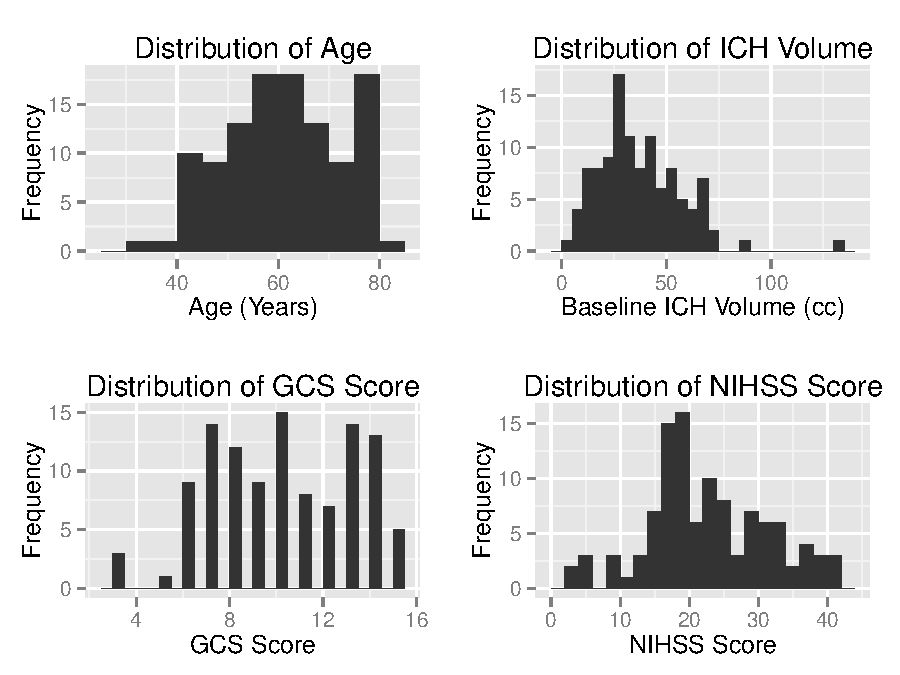
\includegraphics[scale=1]{histdem.pdf}
\end{center}
\caption{Histograms of age (in years), baseline ICH volume (in cc), GCS and NIHSS scores for the patients in the study. We observe that our population is predominantly over $40$ and that are on average 60.8 years of age.  The distribution of baseline ICH has a median of 33cc, with some patients having very large ICH volumes.  GCS scores indicate that a few patients ($N = 3$) with a GCS of $3$ indicating a deep unconsciousness, yet the mean GCS score is $10$.  The distribution of NIHSS scores shows a simlar trend with a mean of $22.1$.   }\label{fig:histdem}
\end{figure}


\begin{figure}[H]
\centering
 \subfloat[\textbf{Original Image} (in native space) with overlaid brain-extraction mask colored in red.  We observe that the mask does not appreciably drop out any areas of the brain nor does it add areas of the skull, eyes, or nose.  ]{
 \label{bet:sso}
 \includegraphics[width=.48\textwidth]{{100-318_20070723_0957_CT_3_CT_Head-_SS_Mask_0.01}.png}
 }
  \hfill
 \subfloat[\textbf{Brain-extracted image} used for re-centering to AC-PC line for SPM8 registration techniques.  ]{
 \label{bet:ss}
 \includegraphics[width=.48\textwidth]{{100-318_20070723_0957_CT_3_CT_Head-_SS_0.01}.png}
}
  \caption{Image~\protect\subref{bet:sso},  displays the original image with the brain-extracted mask in red created from BET. Image~\protect\subref{bet:ss} is the brain extracted image with the mask applied.  We observe that the brain extraction appears to extract only the brain and not extra features.  The image in~\protect\subref{bet:ss} can be used for more quantitative patient-level measurements such as intracranial volume, mean Hounsfield units of areas, intensity-based normalization, and can restrict analyses to only brain tissue and not extracranial areas.}
  \label{fig:bet}
\end{figure}



\begin{figure}[H]
\centering
 \subfloat[\textbf{Native space} where the image looks ``scrunched'' vertically since the slice thicknesses are smaller for the middle and above part of the brain. ]{
 \label{reg:nat1}
 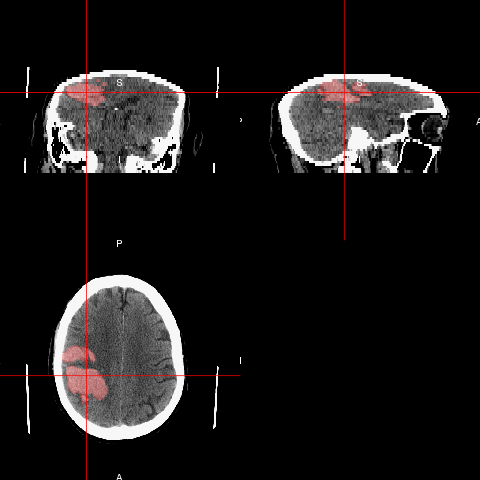
\includegraphics[width=.31\textwidth]{native_100-362_20100126_1926_CT_2_CT_ROUTINE.png}
 }
  \hfill
 \subfloat[\textbf{Registered image} with in template space with hemorrhage mask highlighted in pink. We observe that the brain has been stretched to match the dimensions of the template, yet structures on the patient image look to be in the same areas as that of the template in panel~\protect\subref{reg:temp1}.]{
 \label{reg:co1}
 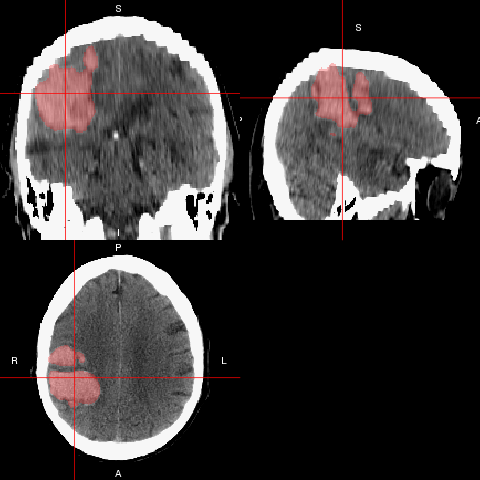
\includegraphics[width=.31\textwidth]{raw_spm_100-362_20100126_1926_CT_2_CT_ROUTINE.png}
}
  \hfill
  \subfloat[\textbf{Template image} with hemorrhage mask overlaid in white.]{
 \label{reg:temp1}
 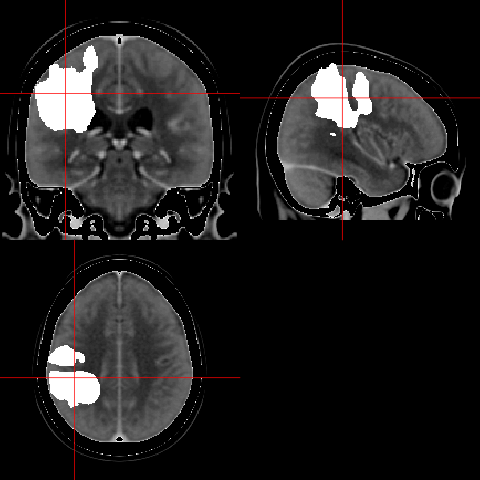
\includegraphics[width=.31\textwidth]{roi_spm_100-362_20100126_1926_CT_2_CT_ROUTINE.png}
} 
% \newline
%  \subfloat[\textbf{Native space} where image acquired tilted and off-center]{
%  \label{reg:nat2}
%  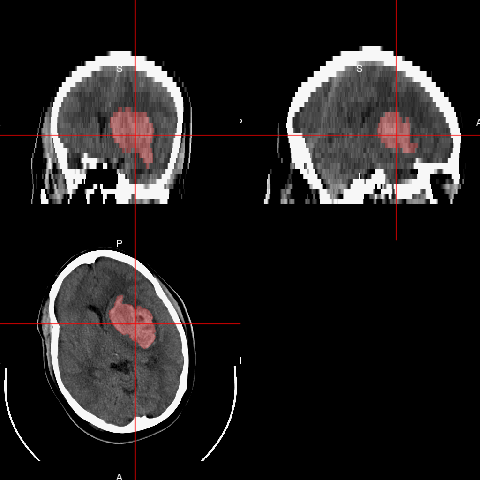
\includegraphics[width=.31\textwidth]{native_223-407_20110522_0119_CT_2_CT_RoutineSpi.png}
% }
%   \hfill
%  \subfloat[\textbf{Registered image} rotated and overlaid hemorrhage mask]{
%  \label{reg:co2}
%  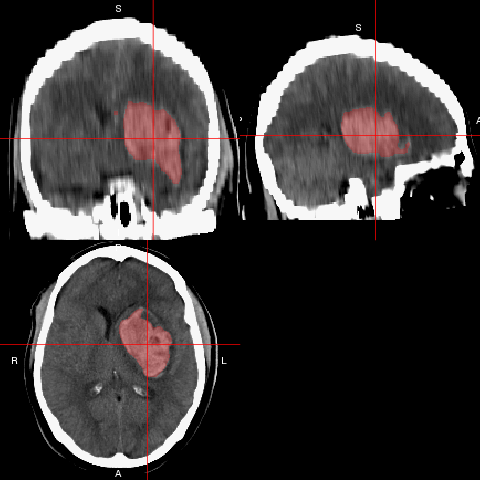
\includegraphics[width=.31\textwidth]{raw_spm_223-407_20110522_0119_CT_2_CT_RoutineSpi.png}
% }
%   \hfill
%   \subfloat[\textbf{Template brain} with hemorrhage mask overlaid]{
%   \label{reg:temp2}
%   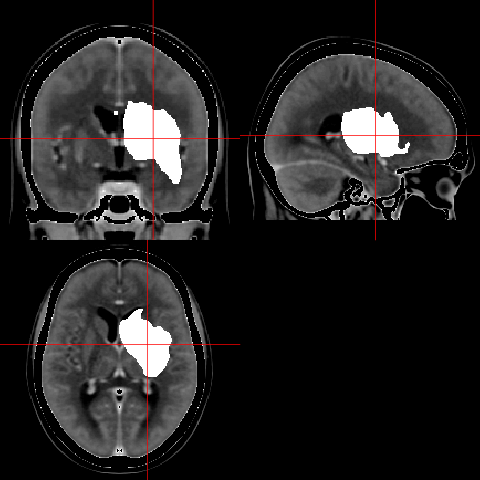
\includegraphics[width=.31\textwidth]{roi_spm_223-407_20110522_0119_CT_2_CT_RoutineSpi.png}
% }
\newline
 \subfloat[\textbf{Native space} where image acquired with homogeneous slice thickness and a small ICH]{
 \label{reg:nat2}
 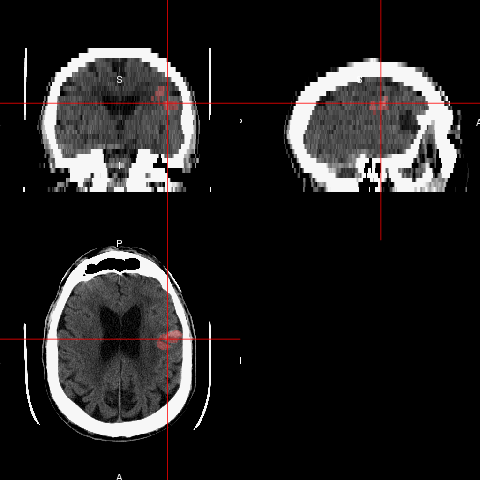
\includegraphics[width=.31\textwidth]{native_191-301_20060201_1148_CT_2_CT_ROUTINE.png}
}
  \hfill
 \subfloat[\textbf{Registered image} in template space with hemorrhage mask highlighted in pink.  We observe the skull (in white) may be scaled during registration, but ventricles int he middle of the brain look similar to those on the template in panel~\protect\subref{reg:temp2}.  ]{
 \label{reg:co2}
 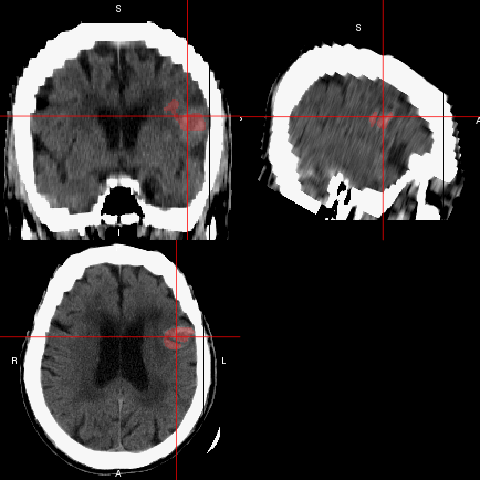
\includegraphics[width=.31\textwidth]{raw_spm_191-301_20060201_1148_CT_2_CT_ROUTINE.png}
}
  \hfill
  \subfloat[\textbf{Template brain} with hemorrhage mask overlaid]{
  \label{reg:temp2}
  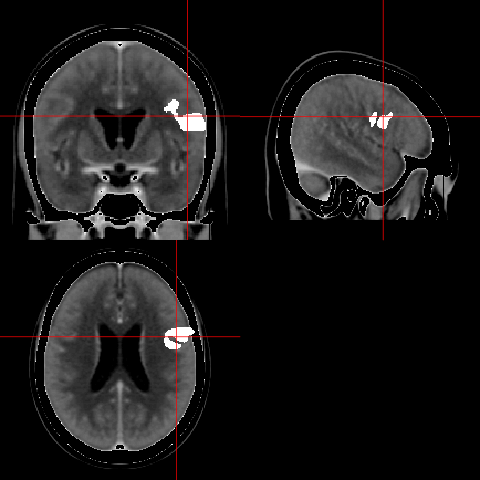
\includegraphics[width=.31\textwidth]{roi_spm_191-301_20060201_1148_CT_2_CT_ROUTINE.png}
}

  \caption{Native (left, panels~\protect\subref{reg:nat1} and \protect\subref{reg:nat2}), template-registered (middle, panels~\protect\subref{reg:co1} and \protect\subref{reg:co2}) images from two patients with template brain for comparison (right, panels~\protect\subref{reg:temp1} and \protect\subref{reg:temp2}).  In image~\protect\subref{reg:nat1} shows an image acquired with variable slice thickness, which can be seen as the top of the brain has smaller voxel sizes (thinner slices) than the bottom of the brain. We see in~\protect\subref{reg:co1}, the template-registered image, that the transformation has scaled the brain to the same size as the template.  We see that similar structures, such as the lateral ventricles, are observed on the same axial slice on the patient-level scan compared to the template image, which indicates adequate registration.  We observe a patient with a small ICH in panel~\protect\subref{reg:nat2}, where we see the registration preserves the hemorrhage with respect to surrounding tissue, but may scale areas, such as the skull around the brain, too much.  
  }
  \label{f:reg}
\end{figure}


\begin{figure}[H]
\centering
  \subfloat[\textbf{Distribution} of proportion of patients with hemorrhage. All voxels with 0 proportion are excluded.]{
  \label{prop:hist}
  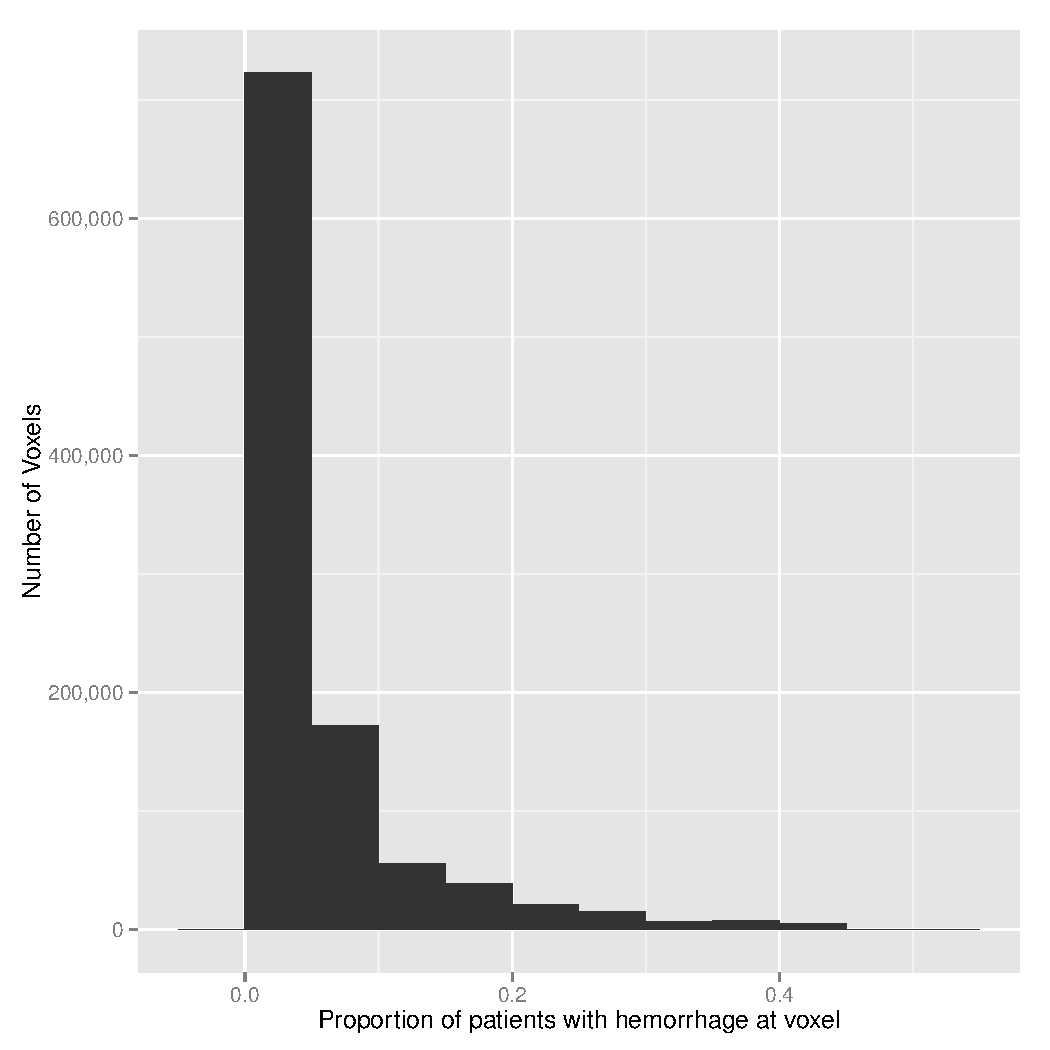
\includegraphics[width=.48\textwidth]{reoriented_Binary_Sum_Image_histogram.pdf}
}
  \subfloat[\textbf{Template brain (MRI T1)} with proportion of hemorrhage overlaid]{
  \label{prop:img}
%   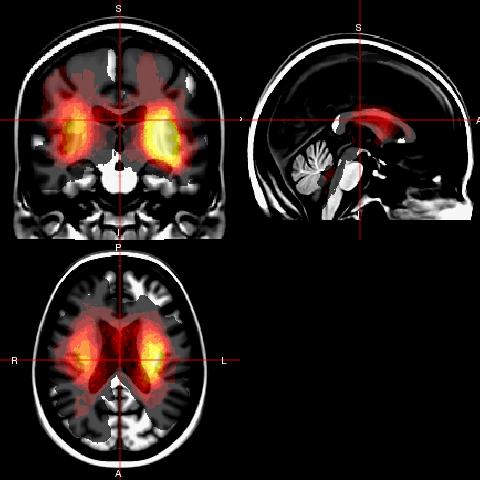
\includegraphics[width=.48\textwidth]{reoriented_Binary_Sum_Image_t1_heat_overlay.png}
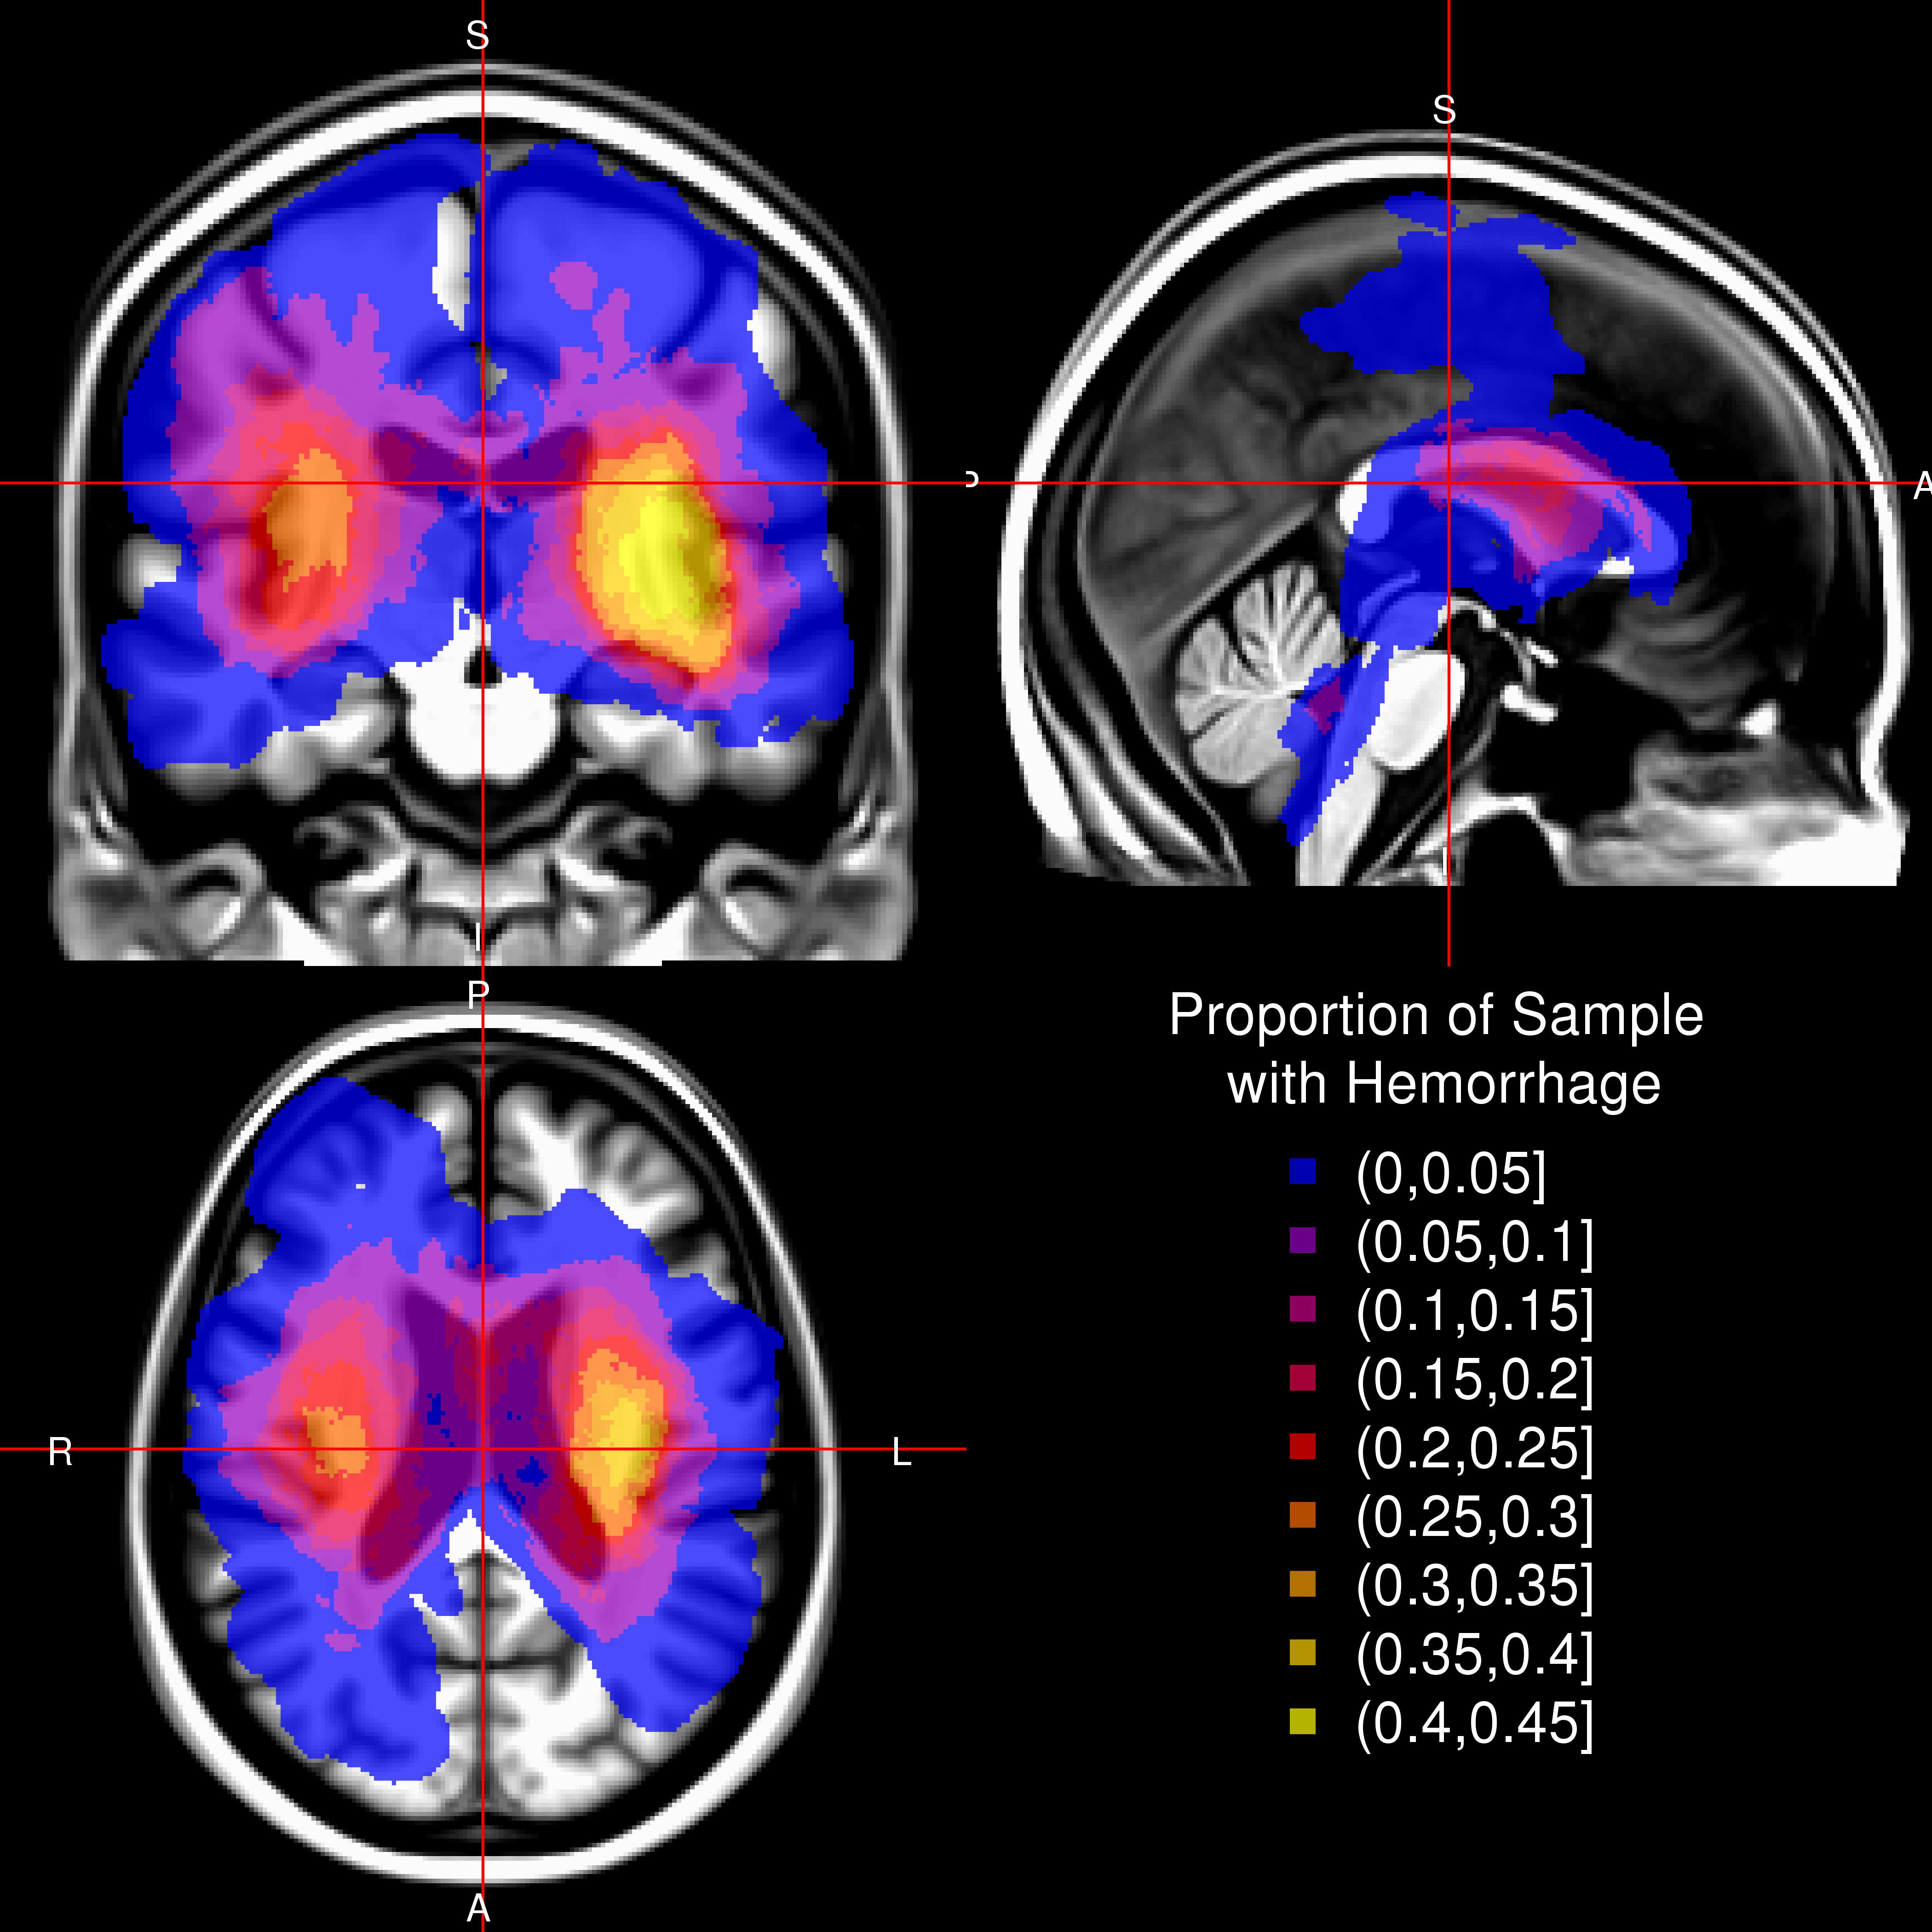
\includegraphics[width=.48\textwidth]{Figure4_Proportion.png}
}

\caption{The histogram of proportion of patients for each voxel that had hemorrhage is presented in Figure~\protect\subref{prop:hist}. Voxels with 0 proportion are excluded.  We observe the majority of voxels have a low prevalence, with a median of 3\%, but some voxels ($V = 5685$) have a high prevalence of over 40\% in this sample.  In Figure~\protect\subref{prop:img}, we present these proportions in a 3D histogram image (radiological convention - right side of image is left side of brain).  Overlaid on the image is a MRI T1 template for spatial orientation and depictions of brain structures.  Brighter values denote a higher percentage of patients that have a hemorrhage at that specific voxel. We see some bi-laterality of the image, but more hemorrhages in the left side of the brain compared to the right.  ICH is also somewhat localized in the middle of the brain, with few extensions in the far anterior and posterior areas of the brain.   The interactive version of this figure is located at \url{http://muschellij2.github.io/CT_Pipeline/index.html}.}
  \label{fig:StrokeHist}
\end{figure}




% \begin{figure}[htbp]
% \centering
%  \subfloat[$\mathcal{M}_1:$ unadjusted]{
%  \label{mods:m1}
%  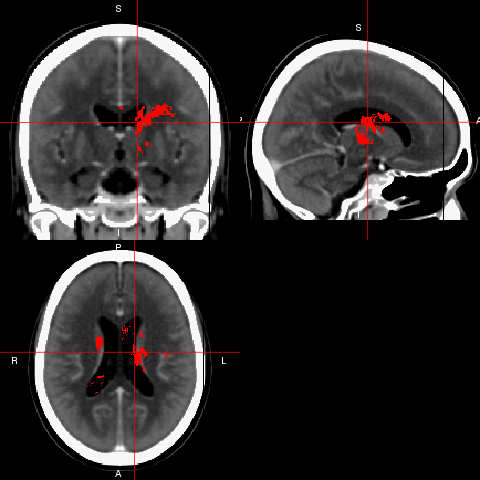
\includegraphics[width=.31\textwidth]{Regression_Map_FDR_red_1_centered.png}
%  }
%   \hfill
%   \subfloat[$\mathcal{M}_2:$ adjusted for Age]{
%  \label{mods:m2}
%  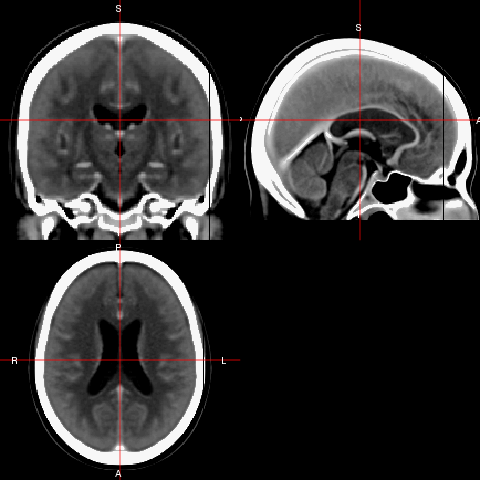
\includegraphics[width=.31\textwidth]{Regression_Map_FDR_red_2_centered.png}
%  }
%   \hfill
%   \subfloat[$\mathcal{M}_3:$ adjusted for Gender]{
%  \label{mods:m3}
%  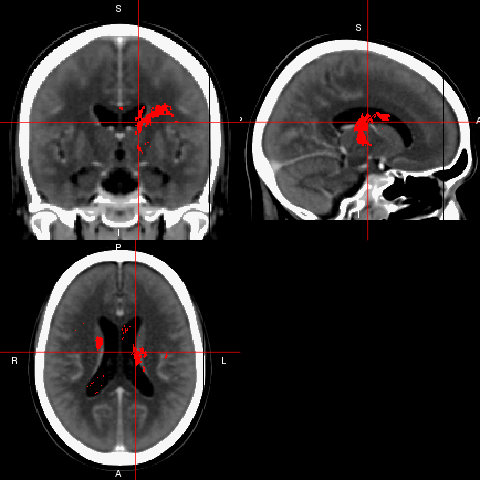
\includegraphics[width=.31\textwidth]{Regression_Map_FDR_red_3_centered.png}
%  }
% \newline
%   \subfloat[$\mathcal{M}_4:$ adjusted for total baseline ICH volume]{
%  \label{mods:m4}
%  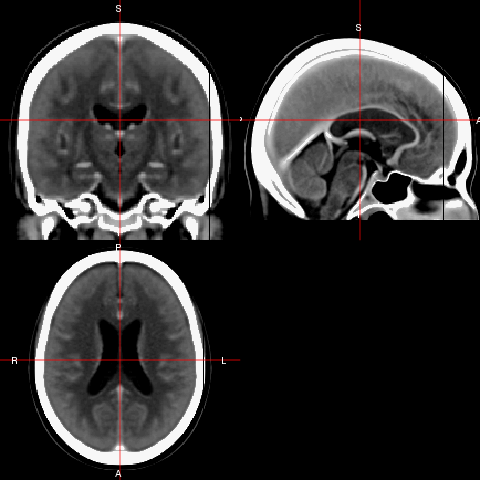
\includegraphics[width=.31\textwidth]{Regression_Map_FDR_red_4_centered.png}
%  }
%   \hfill
%   \subfloat[$\mathcal{M}_5:$ adjusted for Age, Gender, total baseline ICH volume ]{
%  \label{mods:m5}
%  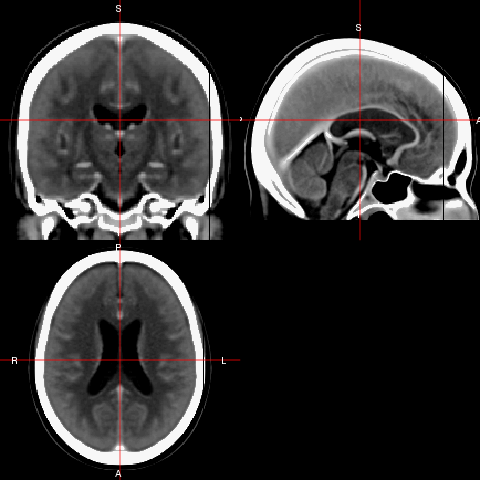
\includegraphics[width=.31\textwidth]{Regression_Map_FDR_red_5_centered.png}
%  }
%   \hfill
%   \subfloat[$\mathcal{M}_6$: voxel-wise Wilcoxon rank-sum test for NIHSS distribution]{
%  \label{mods:m6}
%  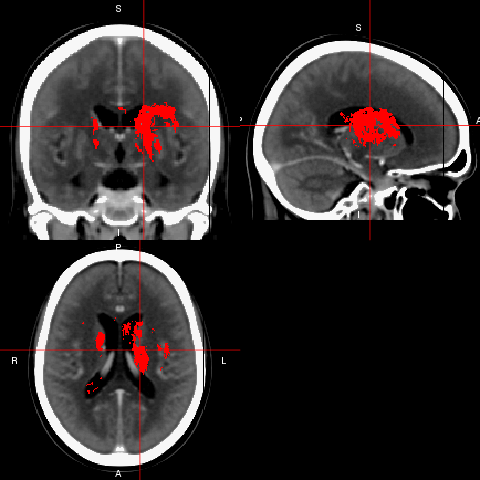
\includegraphics[width=.31\textwidth]{Regression_Map_FDR_red_6_centered.png}
%  } 
  
%   \caption{FDR-corrected significant p-values for the $6$ models.  Voxel-wise p-values were adjusted using an FDR of $.05$, based on the $nuniq.rows$ unique comparisons.  We see that in the unadjusted linear model (figure~\protect\subref{mods:m1}) and after adjusting for gender (figure~\protect\subref{mods:m3}) there are significant voxels on the left and right of the brain, near the ventricles.  In models adjusting for age (figure~\protect\subref{mods:m2}), or total baseline ICH volume (figure~\protect\subref{mods:m4}), or both (figure~\protect\subref{mods:m5}), no voxels are found significantly related to NIHSS after adjustment and FDR-correction.  Also, we see a higher number of voxels deemed significant using the Wilcoxon rank-sum test (figure~\protect\subref{mods:m6}). Slices are presented at the centroid of the mask of the significant voxels. }
%   \label{f:mods}
% \end{figure}





% \begin{figure}[htbp]
% \centering
%   \subfloat[Top $1000$ voxels]{
%  \label{pvals:1000}
%  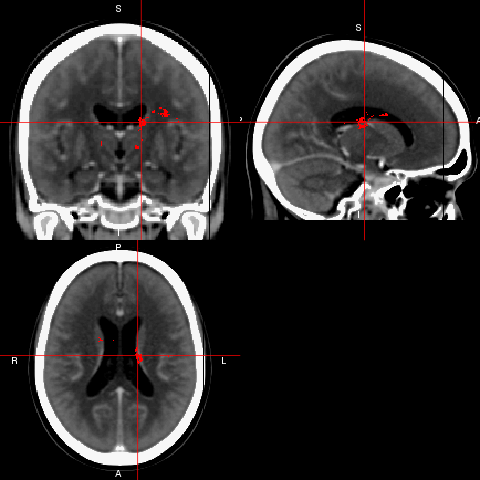
\includegraphics[width=.31\textwidth]{Top_1000_pvalues.png}
%  }
%   \hfill
%   \subfloat[Top $2000$ voxels]{
%  \label{pvals:2000}
%  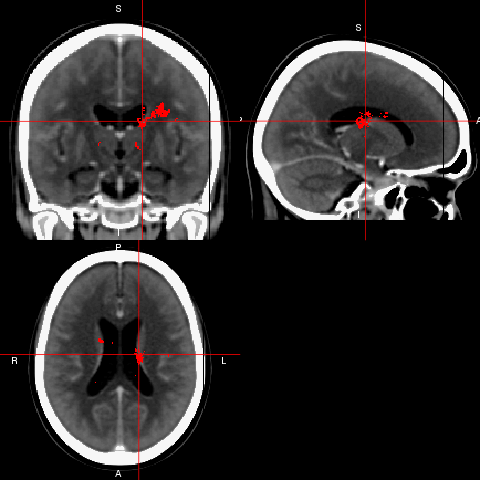
\includegraphics[width=.31\textwidth]{Top_2000_pvalues.png}
%  }
%   \hfill
%   \subfloat[Top $3000$ voxels]{
%  \label{pvals:3000}
%  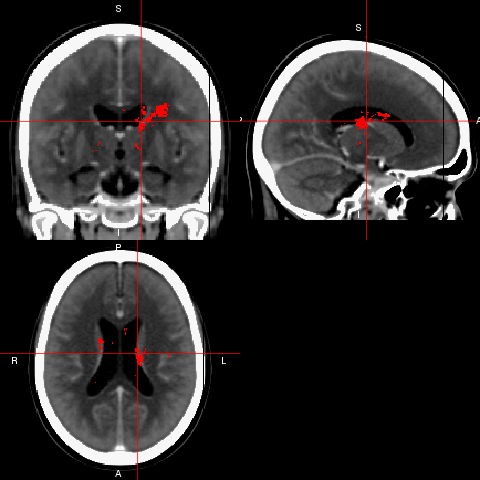
\includegraphics[width=.31\textwidth]{Top_3000_pvalues.png}
%  }
% \newline
%   \subfloat[Voxels with p-values $< .05$ ]{
%  \label{pvals:.05}
%  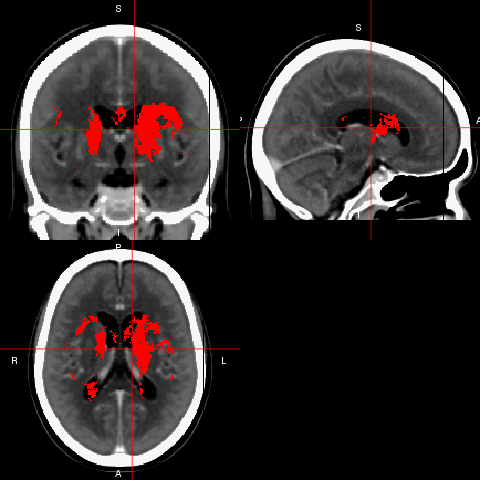
\includegraphics[width=.31\textwidth]{Top_47736_pvalues.png}
%  }
%   \hfill
%   \subfloat[Voxels with p-values $< .01$ ]{
%  \label{pvals:.01}
%  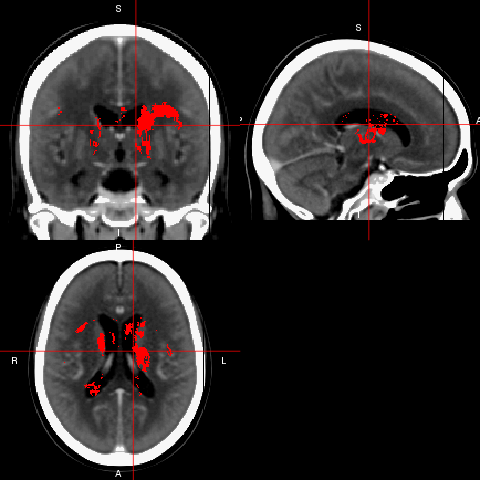
\includegraphics[width=.31\textwidth]{Top_19047_pvalues.png}
%  }
%   \hfill
%   \subfloat[Voxels with p-values $< .001$ ]{
%  \label{pvals:.001}
%  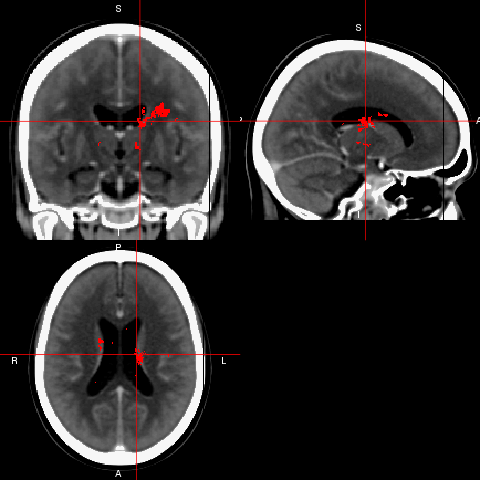
\includegraphics[width=.31\textwidth]{Top_2422_pvalues.png}
%  } 
  
%   \caption{Region of Interest (ROI) based on rank of voxel p-value (top row, \protect\subref{pvals:1000}, \protect\subref{pvals:2000}, \protect\subref{pvals:3000}) or thresholding p-value at $.05$ \protect\subref{pvals:.05}, $.01$ \protect\subref{pvals:.01}, $.001$ \protect\subref{pvals:.001} for the unadjusted model with NIHSS score as the functional outcome.}
%   \label{f:roi}
% \end{figure}




\begin{figure}[H]
\centering
 \subfloat[$\mathcal{M}_1:$ unadjusted]{
 \label{mods:m1}
 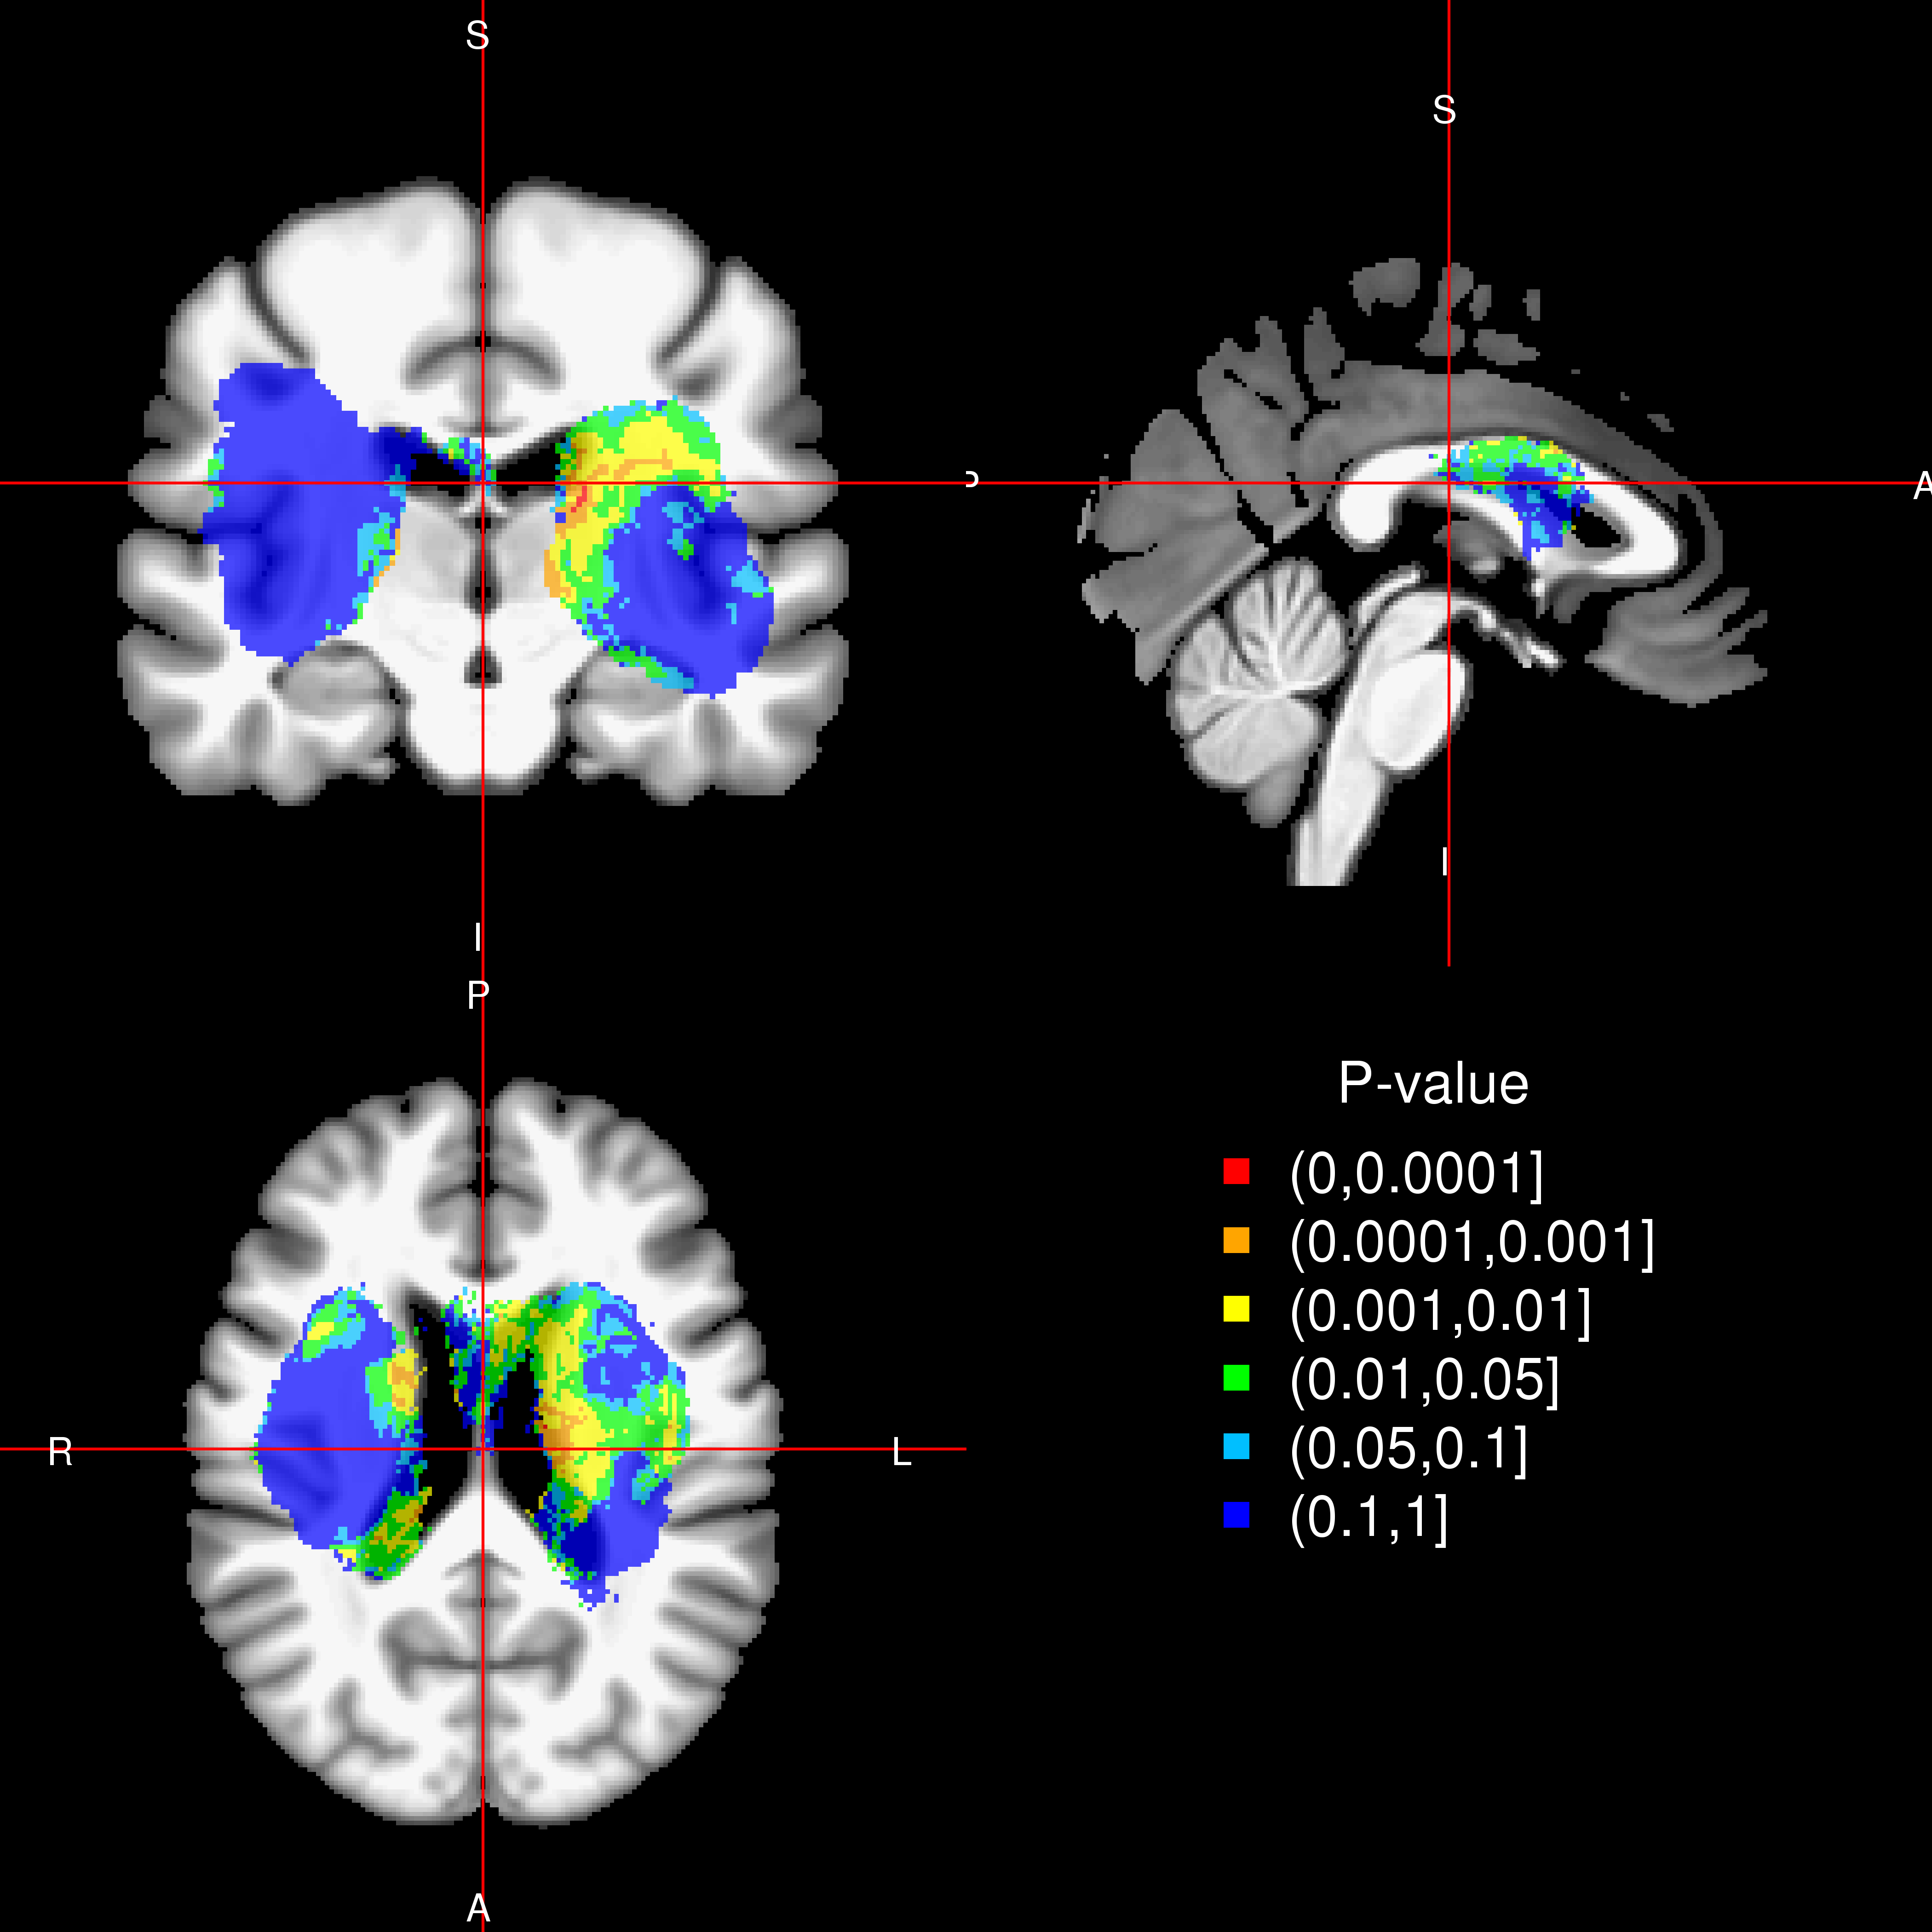
\includegraphics[width=.31\textwidth]{Regression_Map_heatcol1_t1.png}
 }
  \hfill
  \subfloat[$\mathcal{M}_2:$ adjusted for Age]{
 \label{mods:m2}
 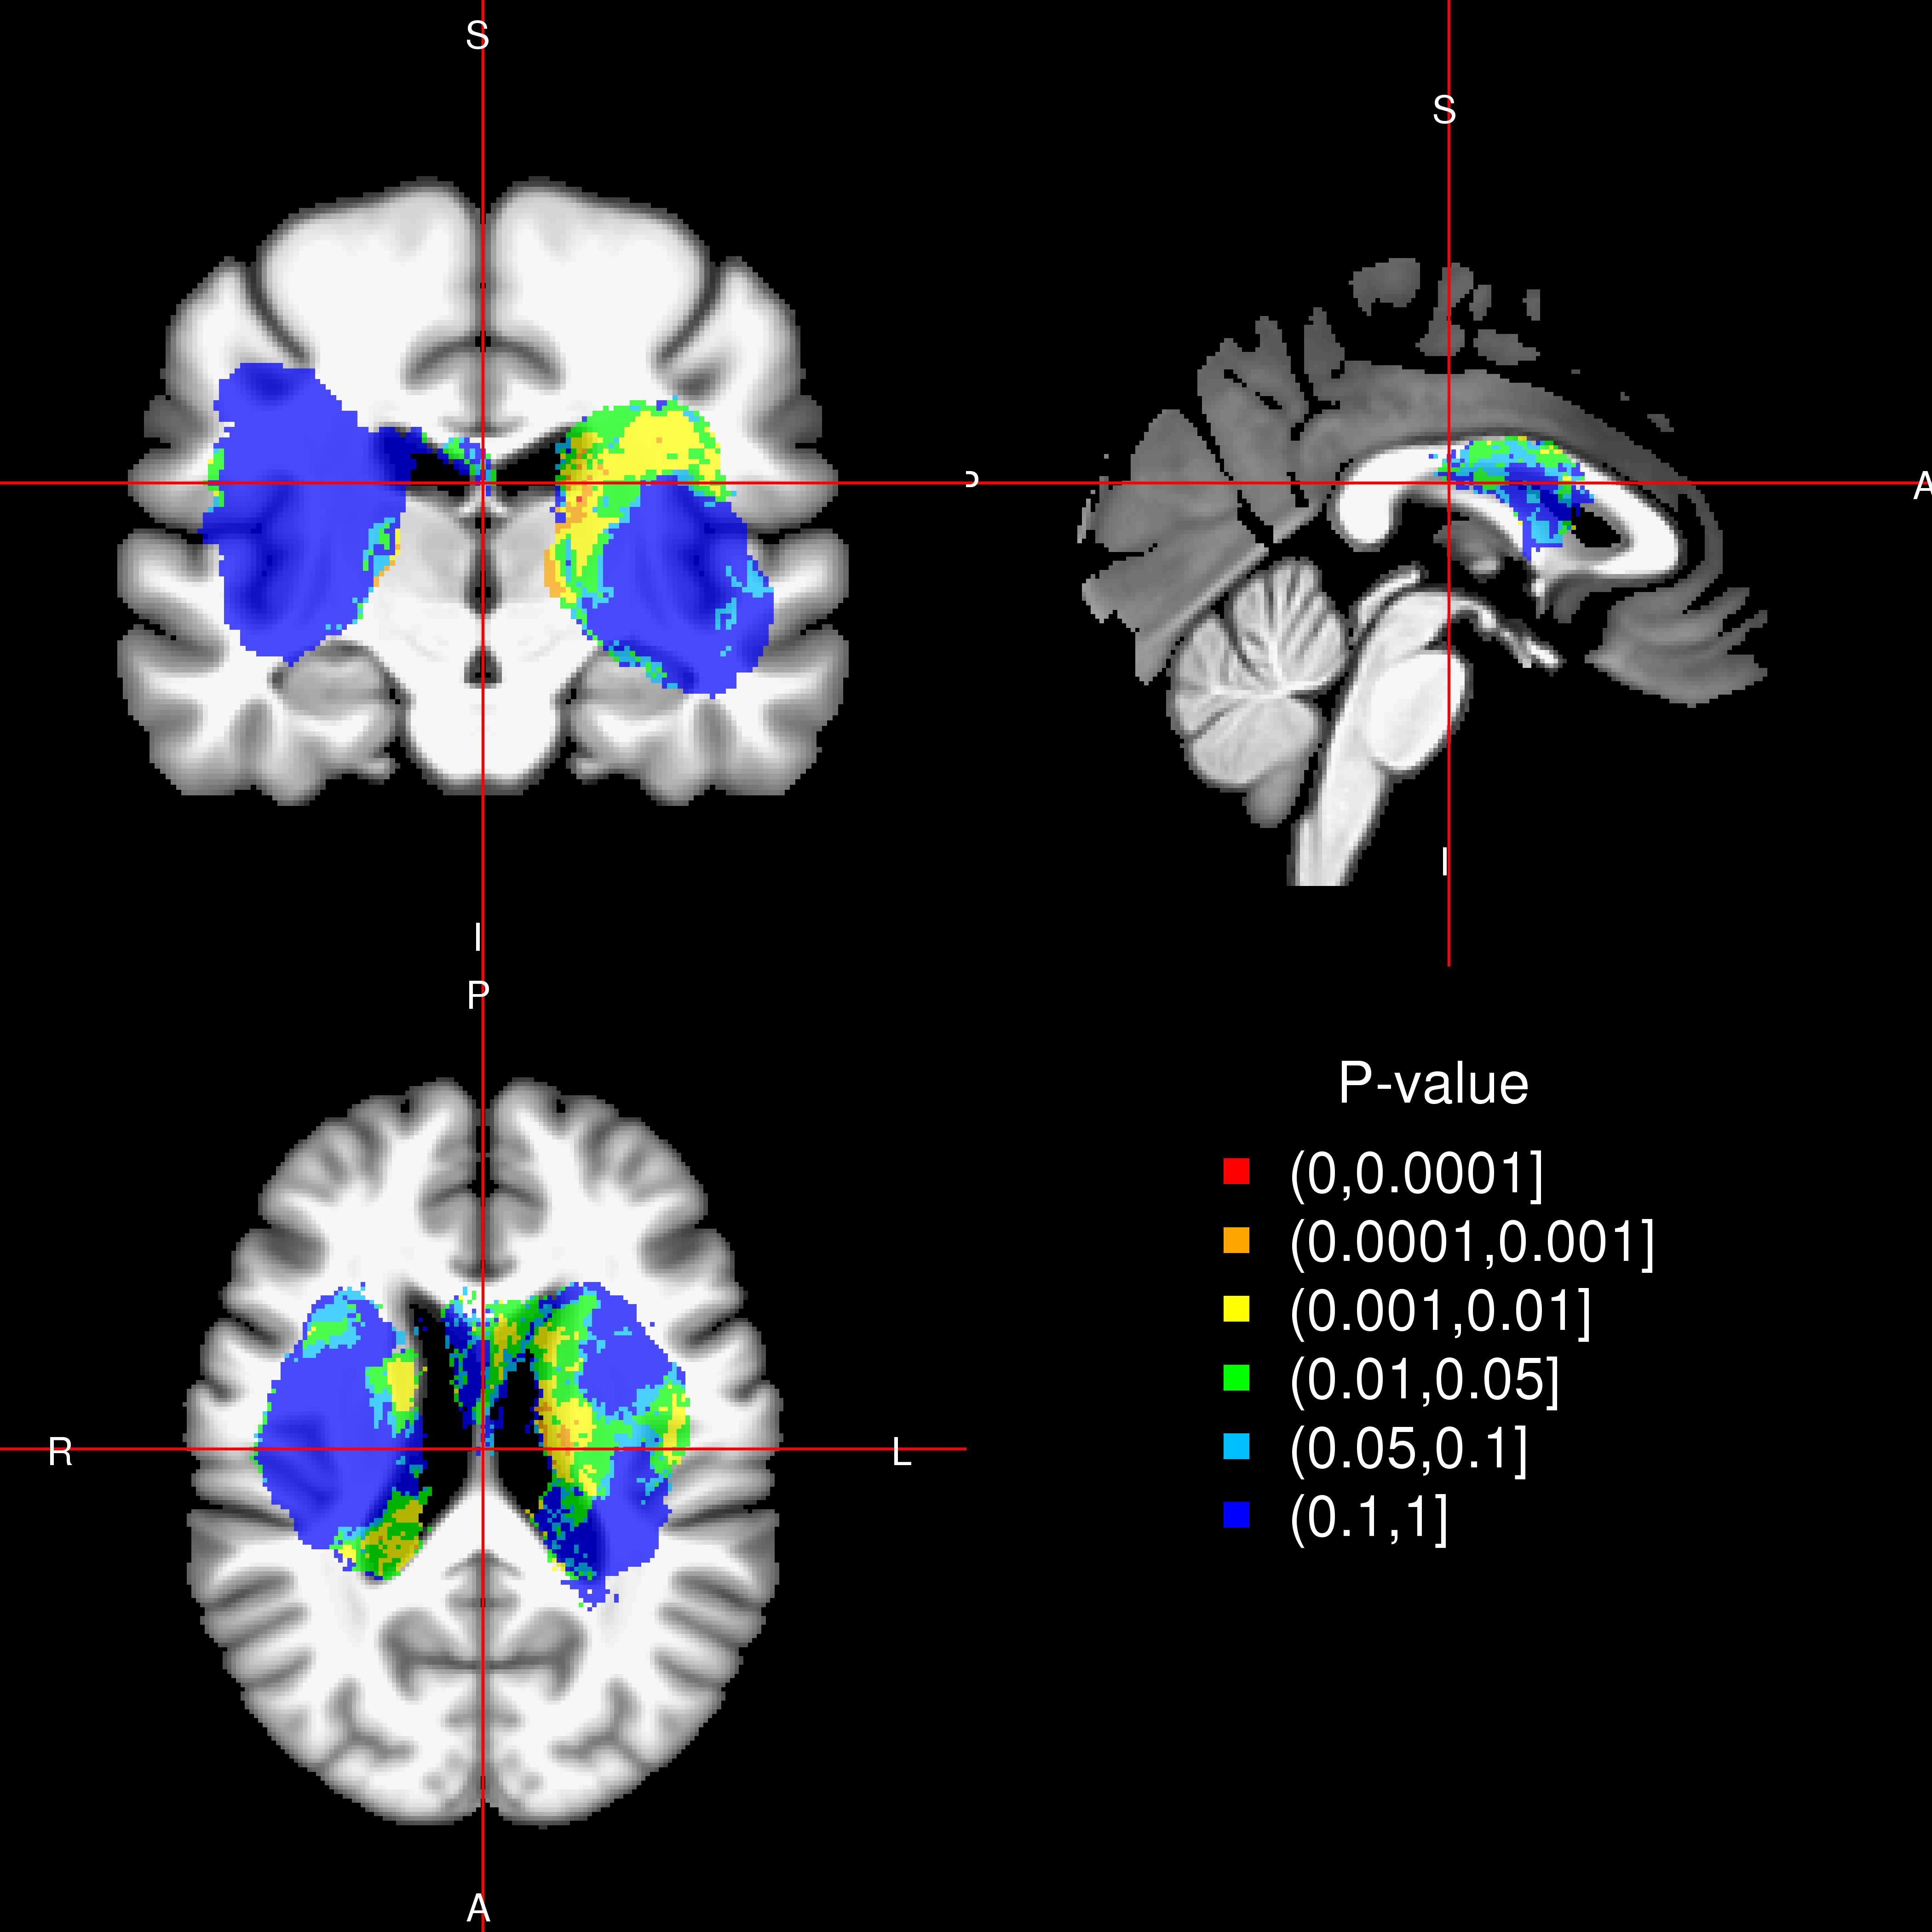
\includegraphics[width=.31\textwidth]{Regression_Map_heatcol2_t1.png}
 }
  \hfill
  \subfloat[$\mathcal{M}_3:$ adjusted for Gender]{
 \label{mods:m3}
 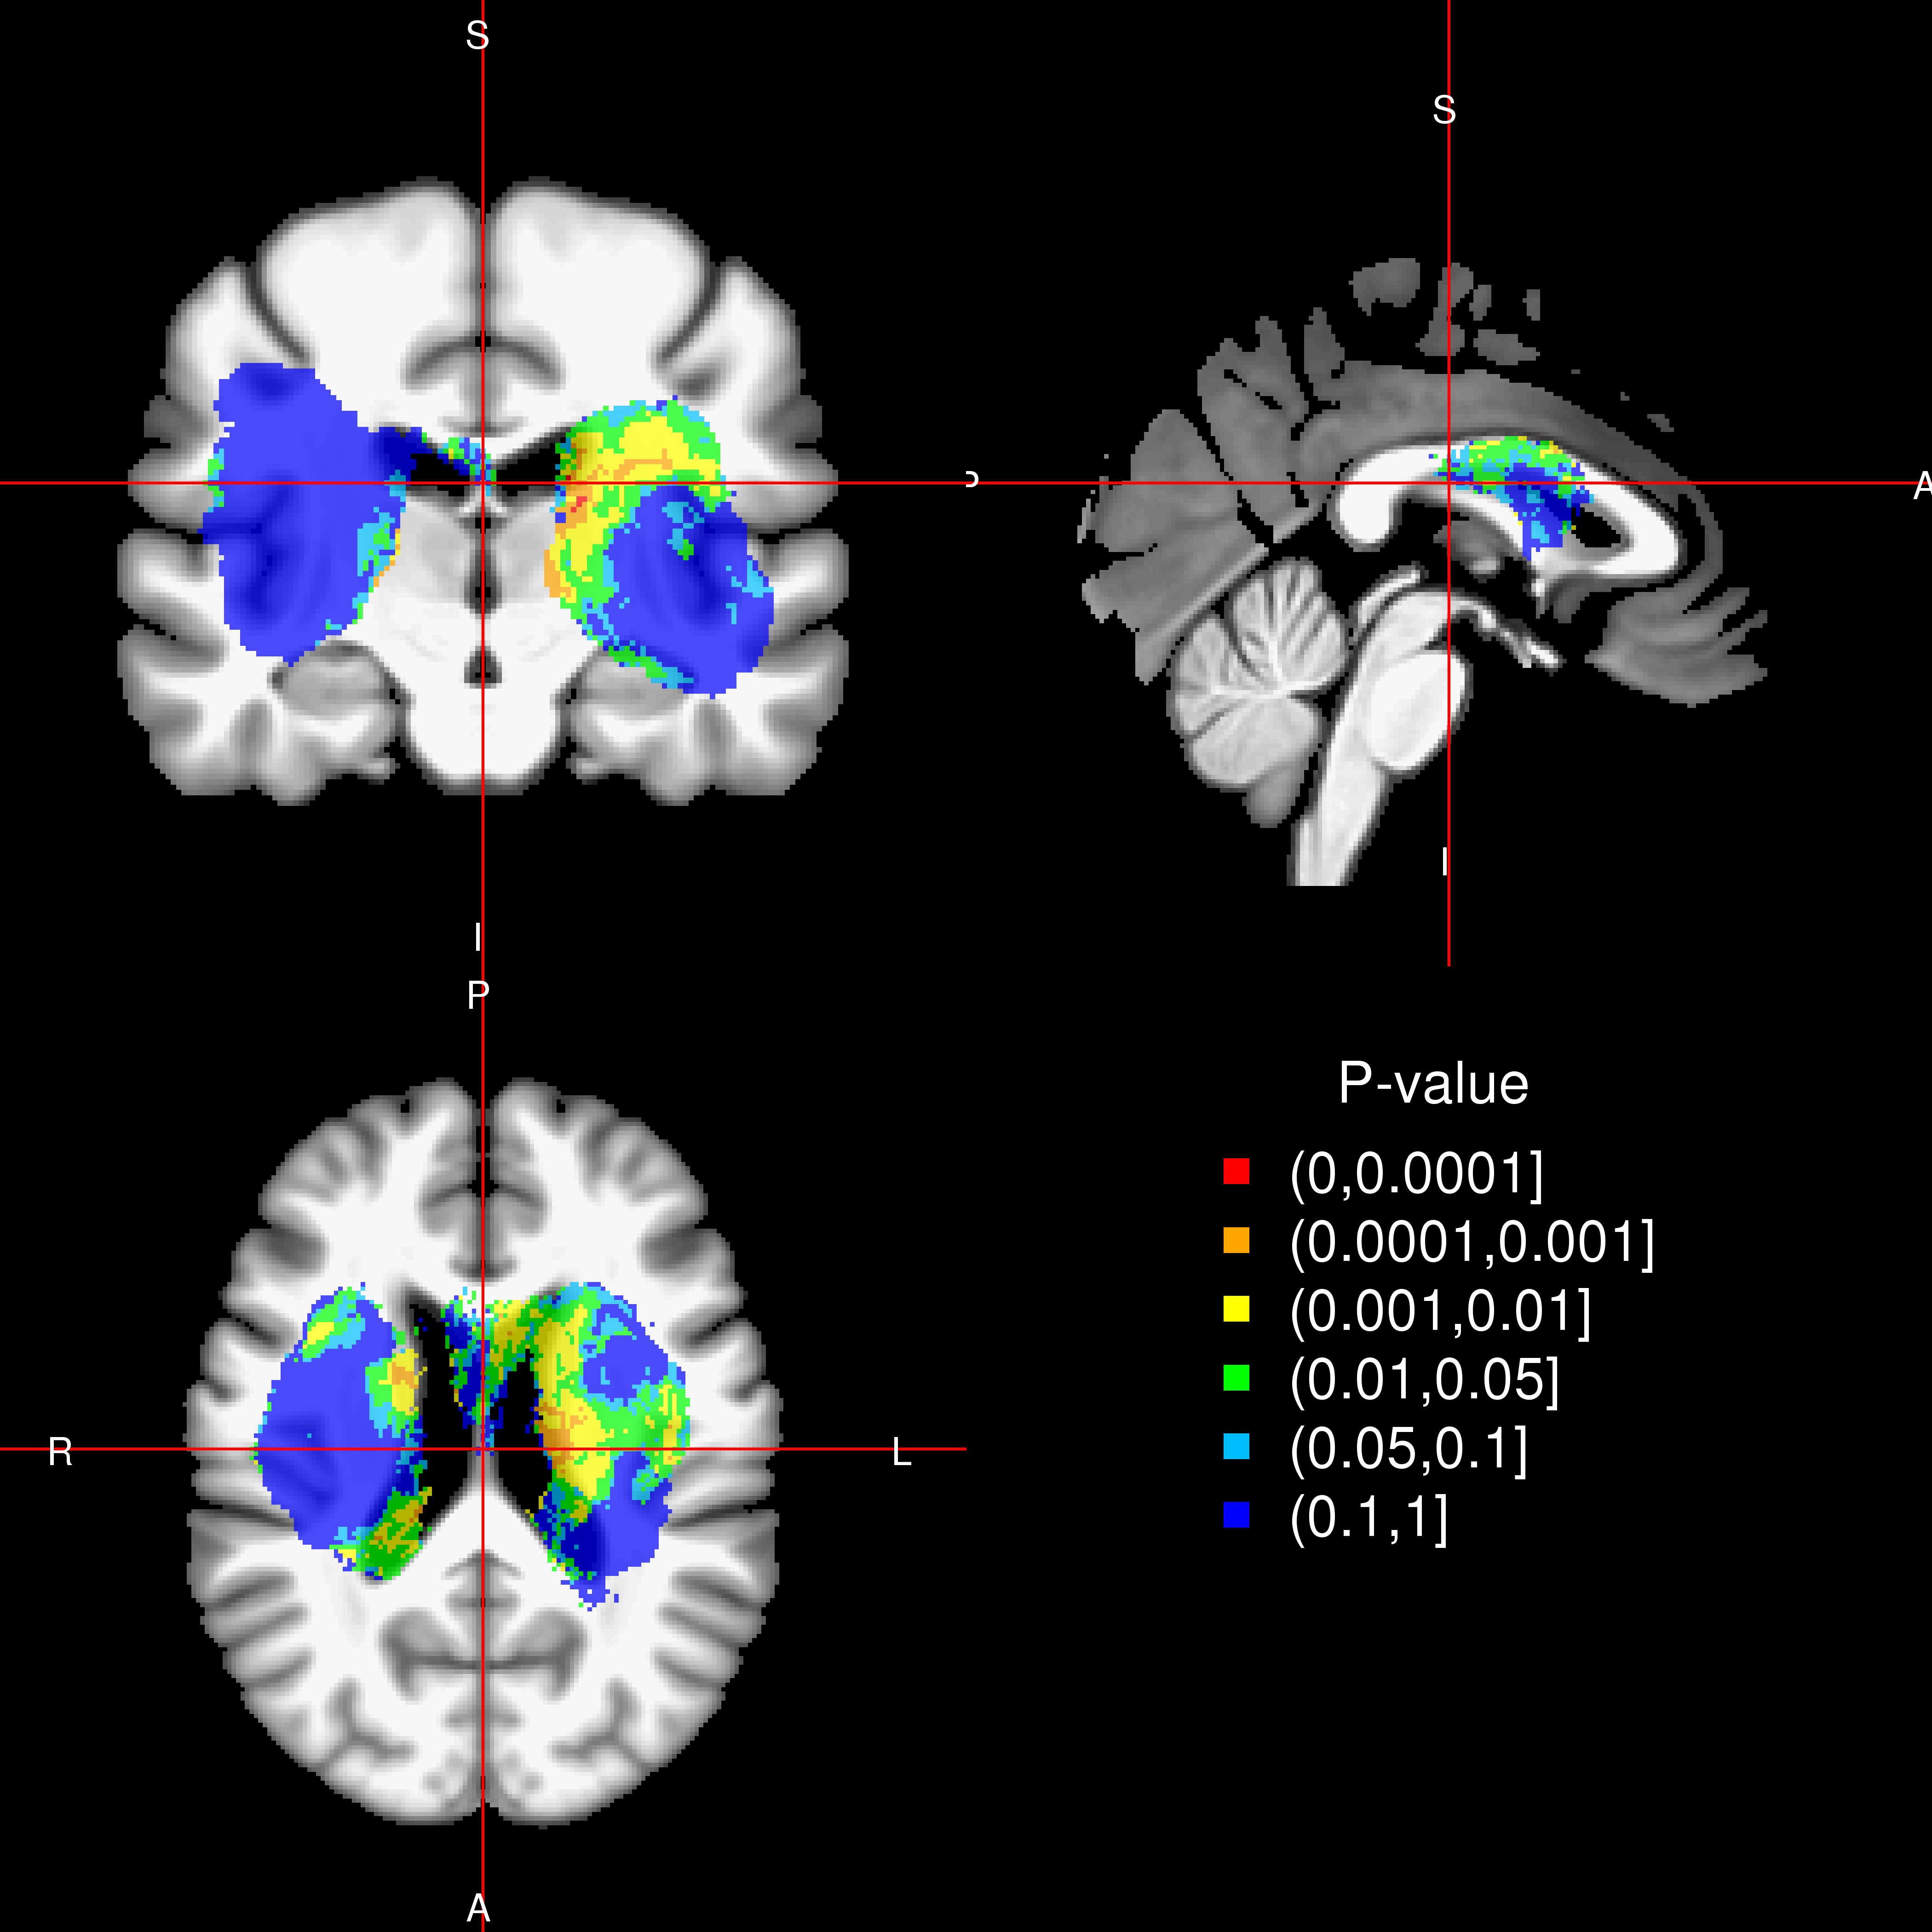
\includegraphics[width=.31\textwidth]{Regression_Map_heatcol3_t1.png}
 }
\newline
  \subfloat[$\mathcal{M}_4:$ adjusted for total baseline ICH volume]{
 \label{mods:m4}
 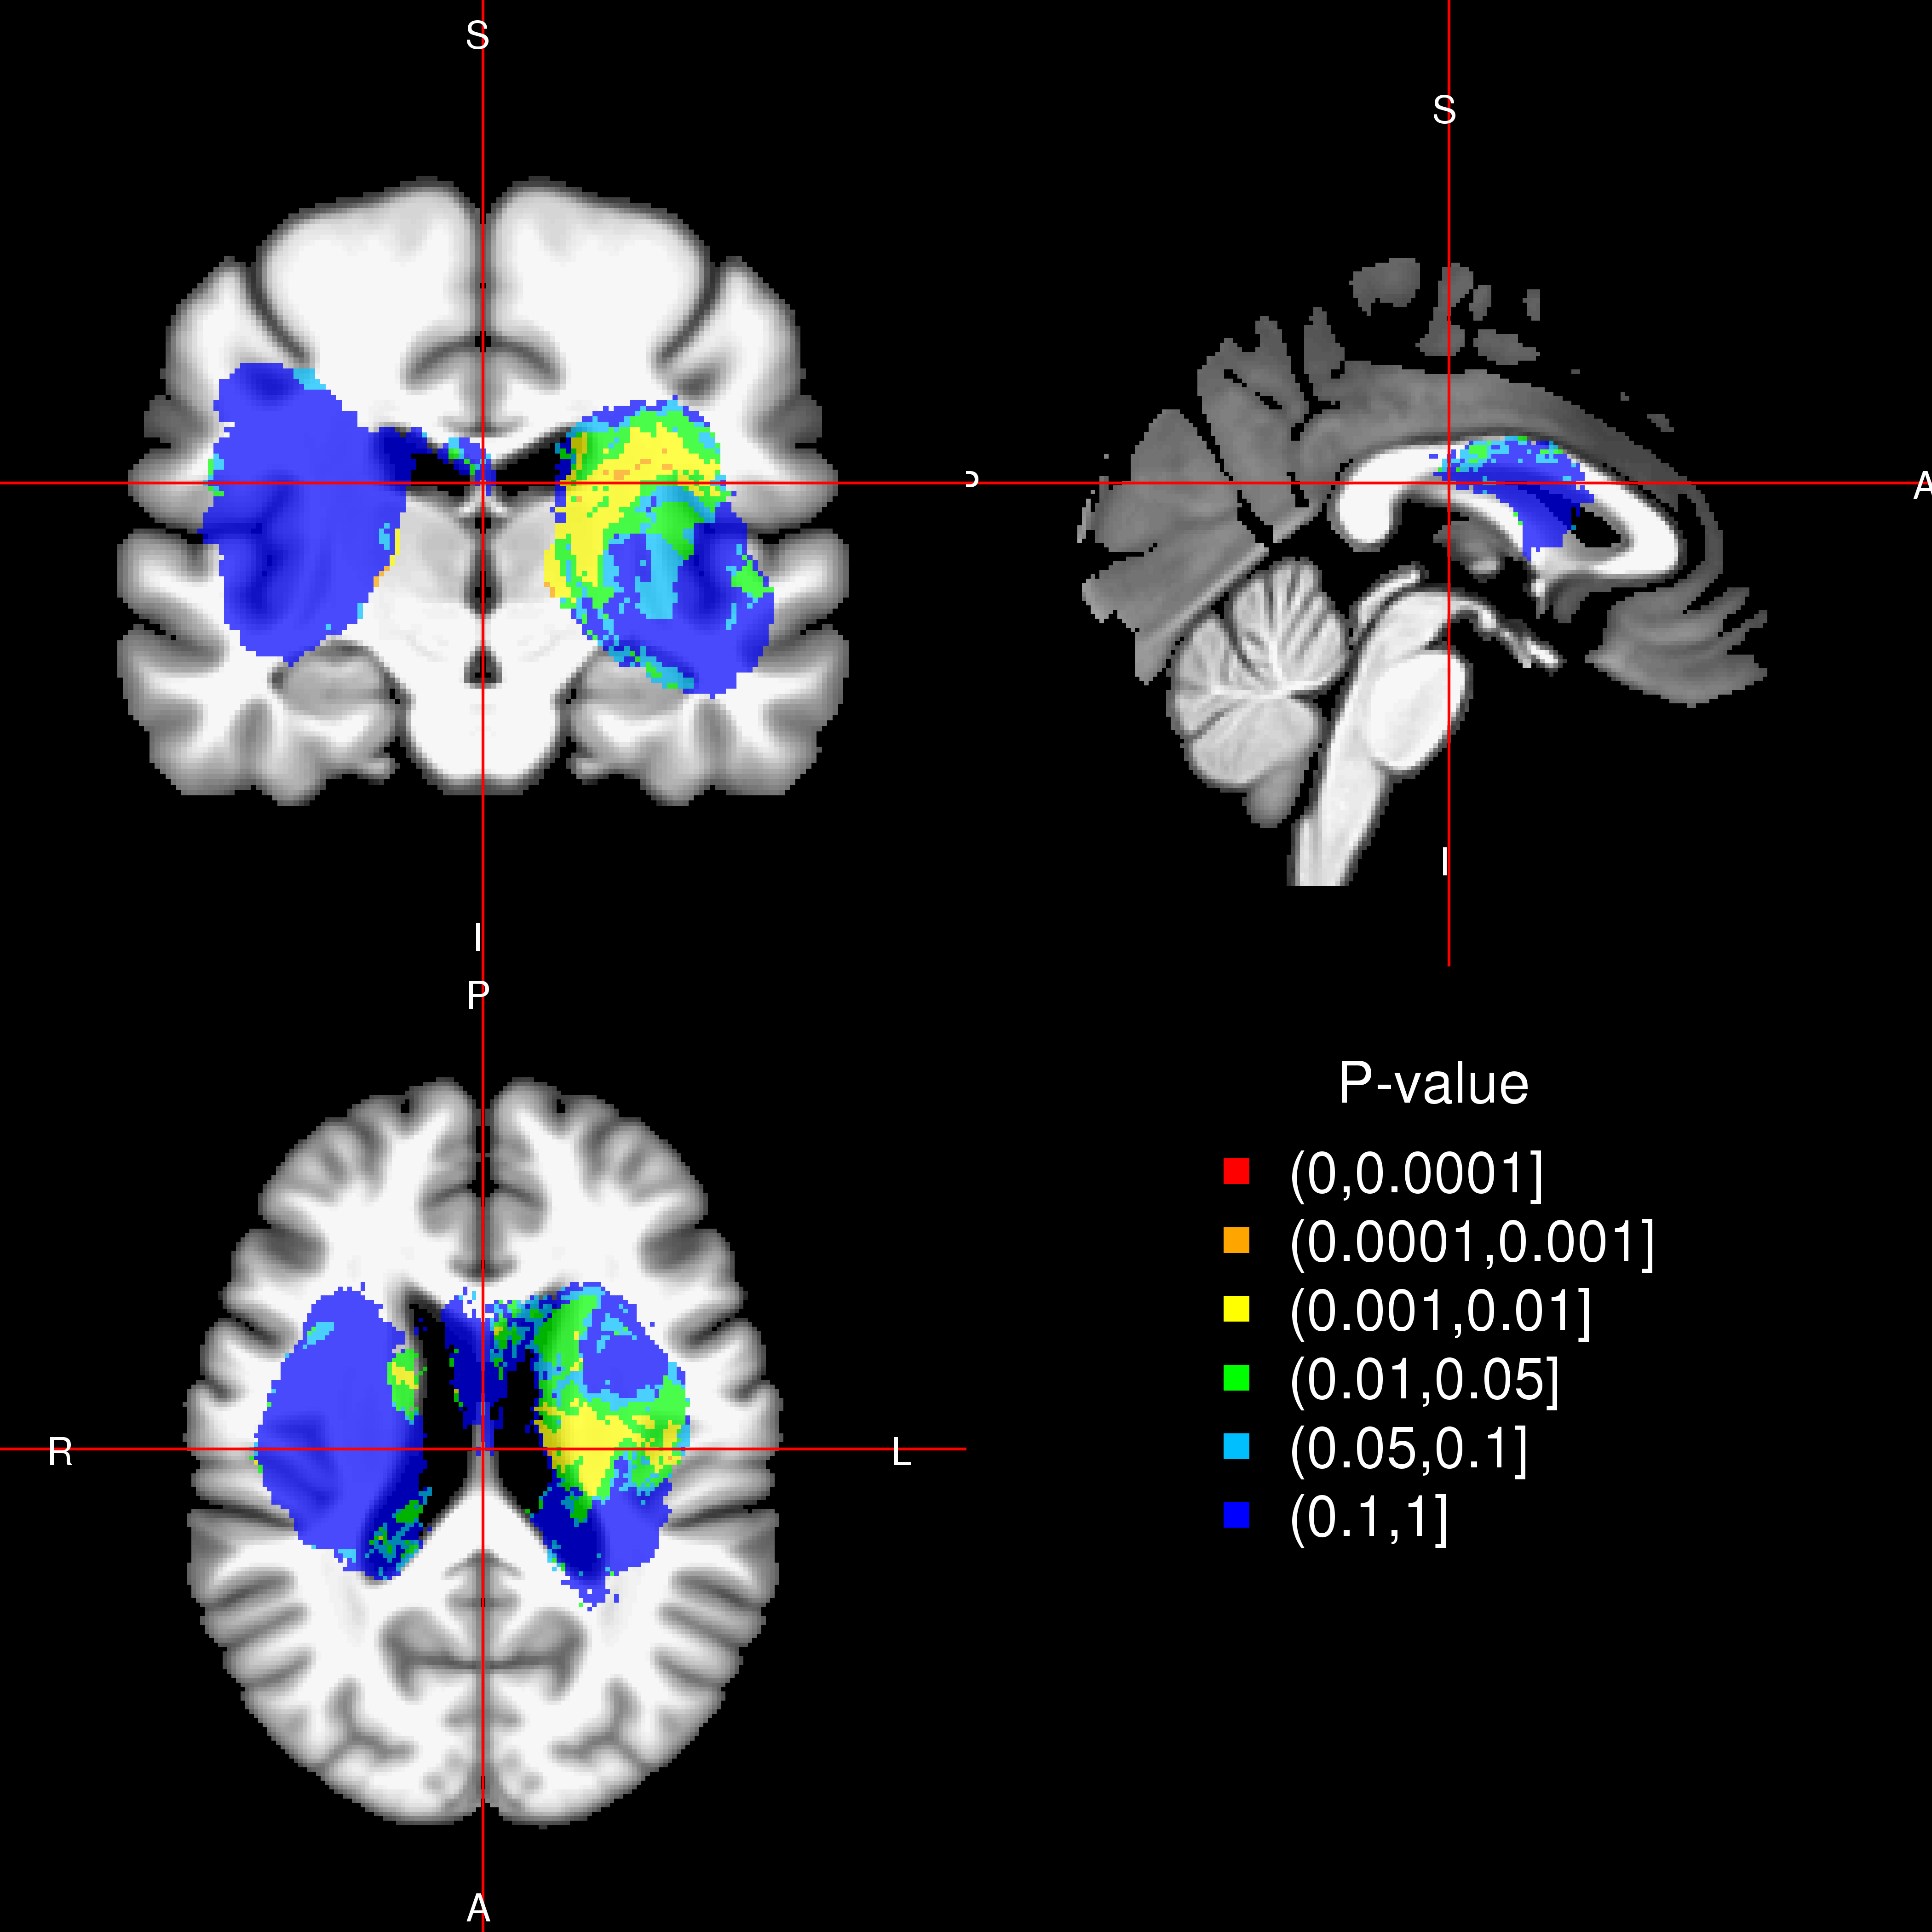
\includegraphics[width=.31\textwidth]{Regression_Map_heatcol4_t1.png}
 }
  \hfill
  \subfloat[$\mathcal{M}_5:$ adjusted for Age, Gender, total baseline ICH volume ]{
 \label{mods:m5}
 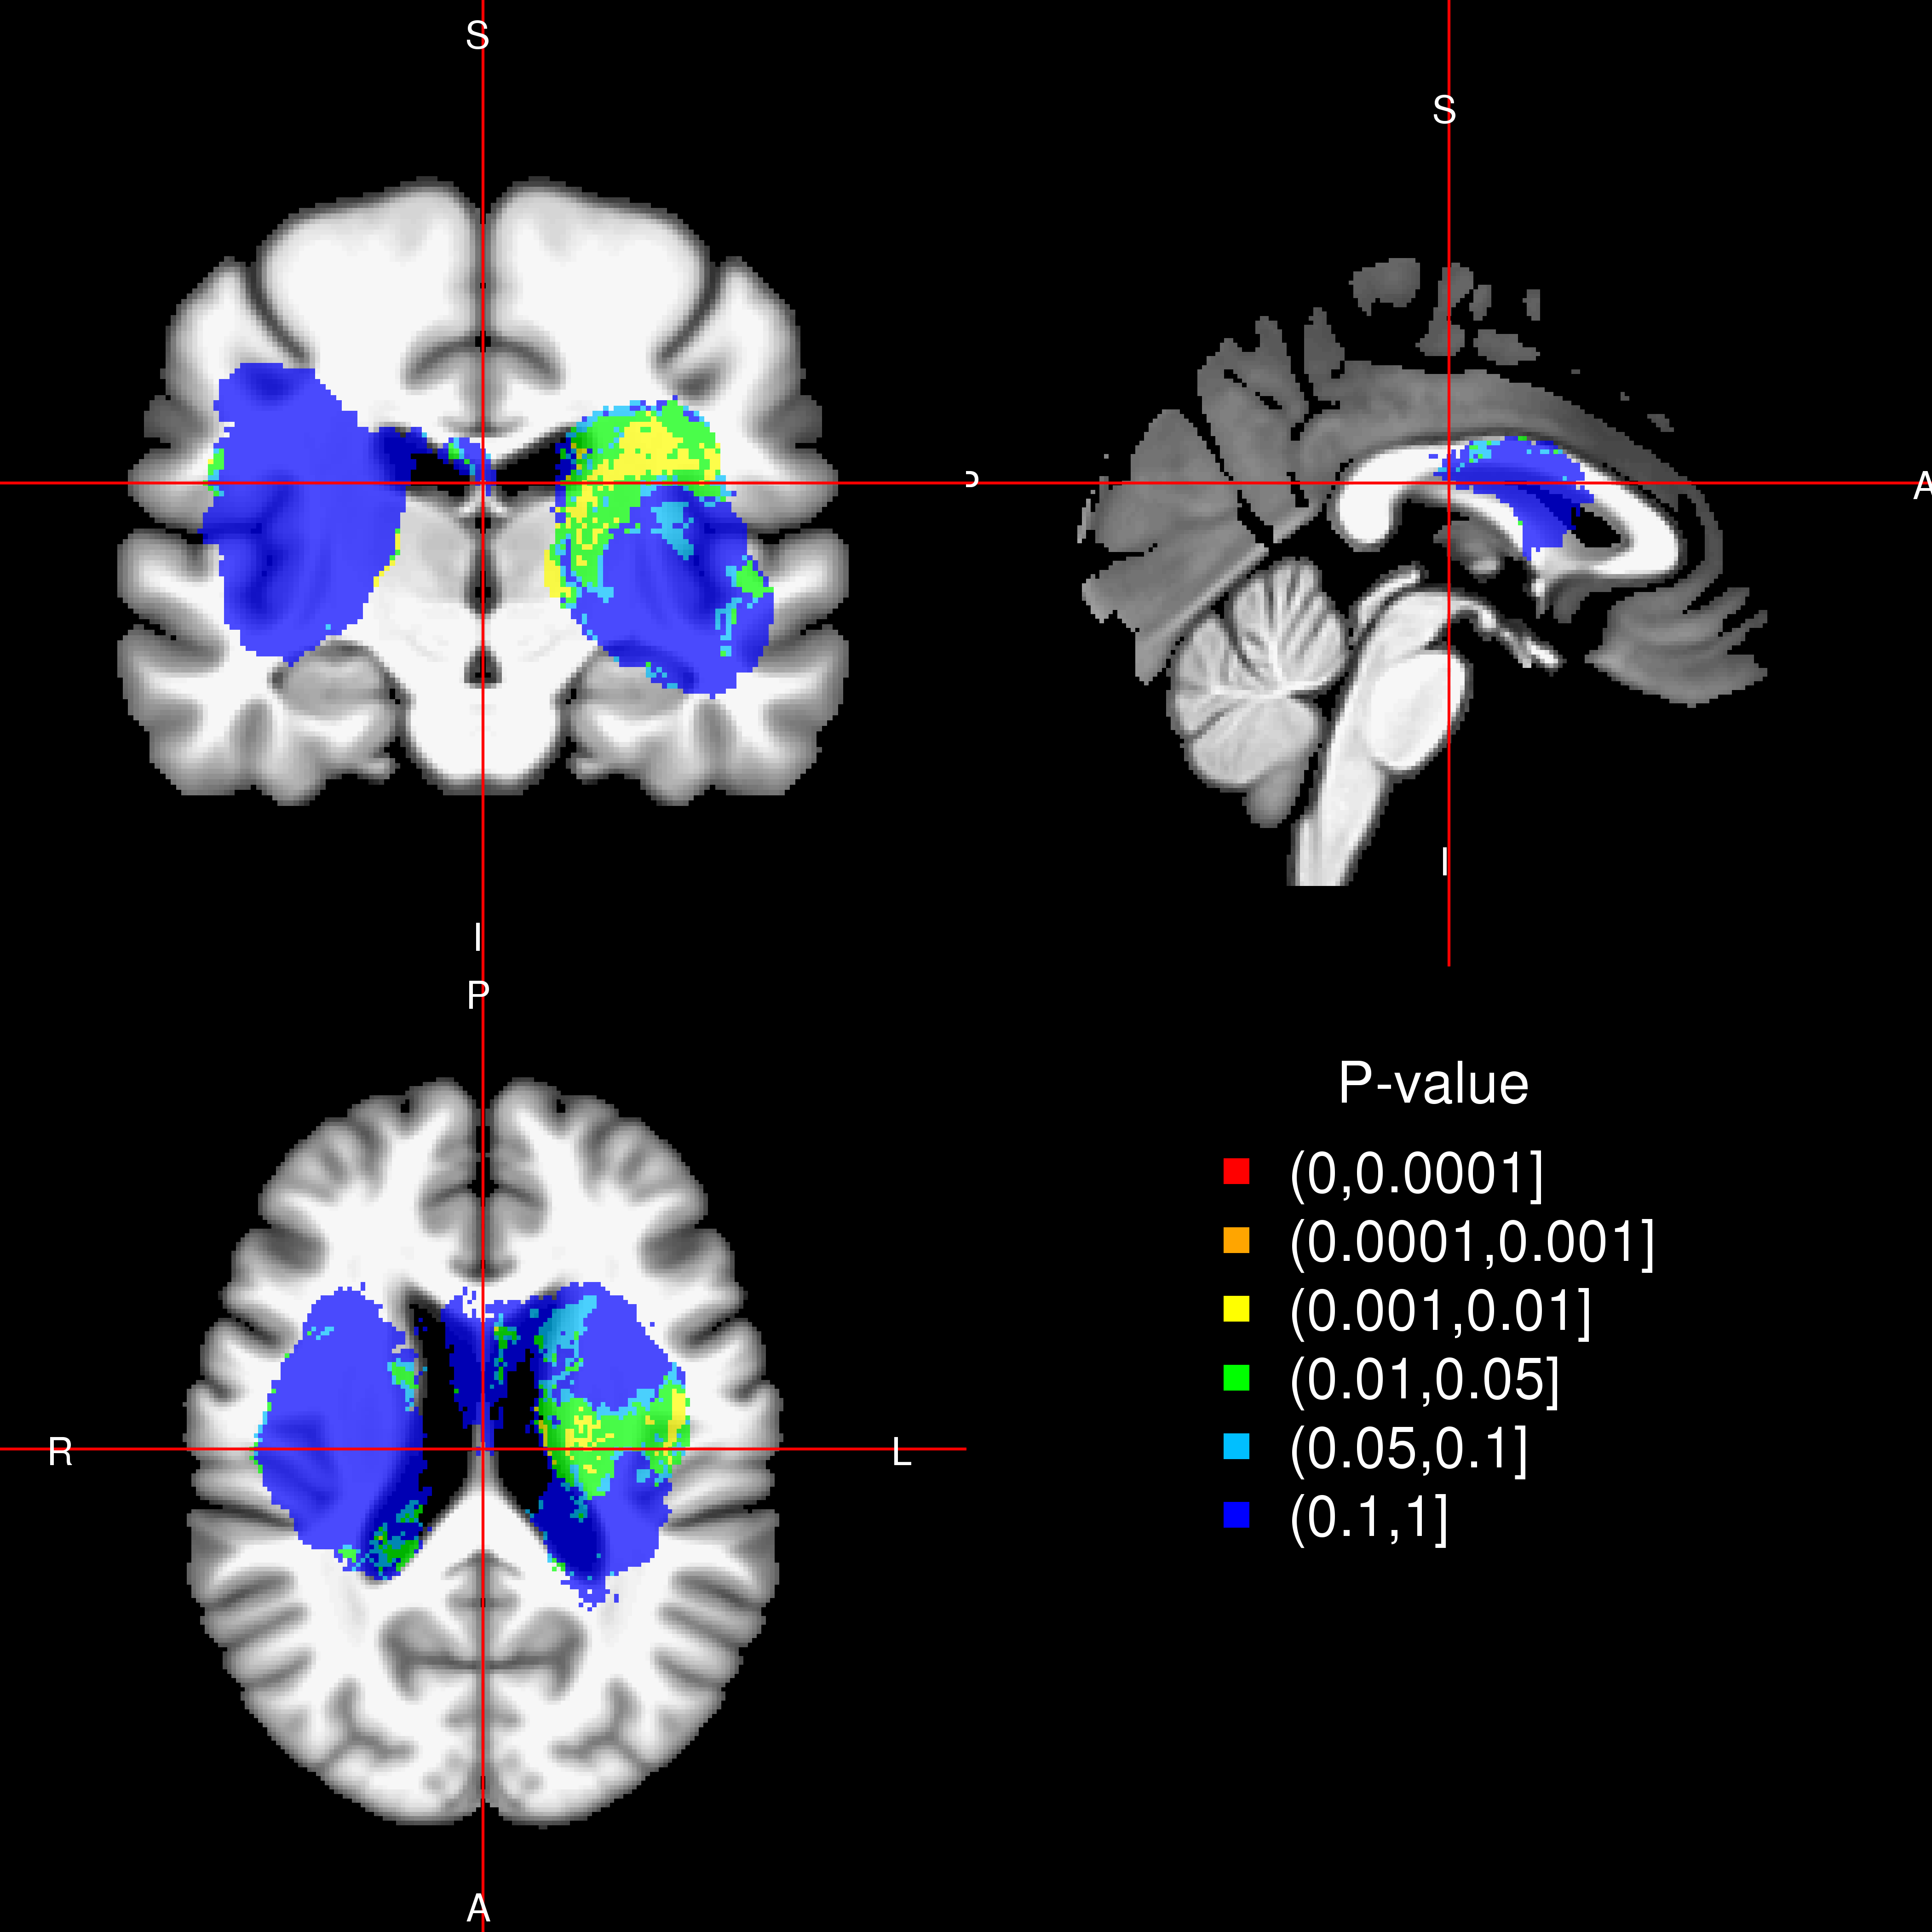
\includegraphics[width=.31\textwidth]{Regression_Map_heatcol5_t1.png}
 }
  \hfill
  \subfloat[$\mathcal{M}_6$: voxel-wise Wilcoxon rank-sum test for NIHSS score distribution]{
 \label{mods:m6}
 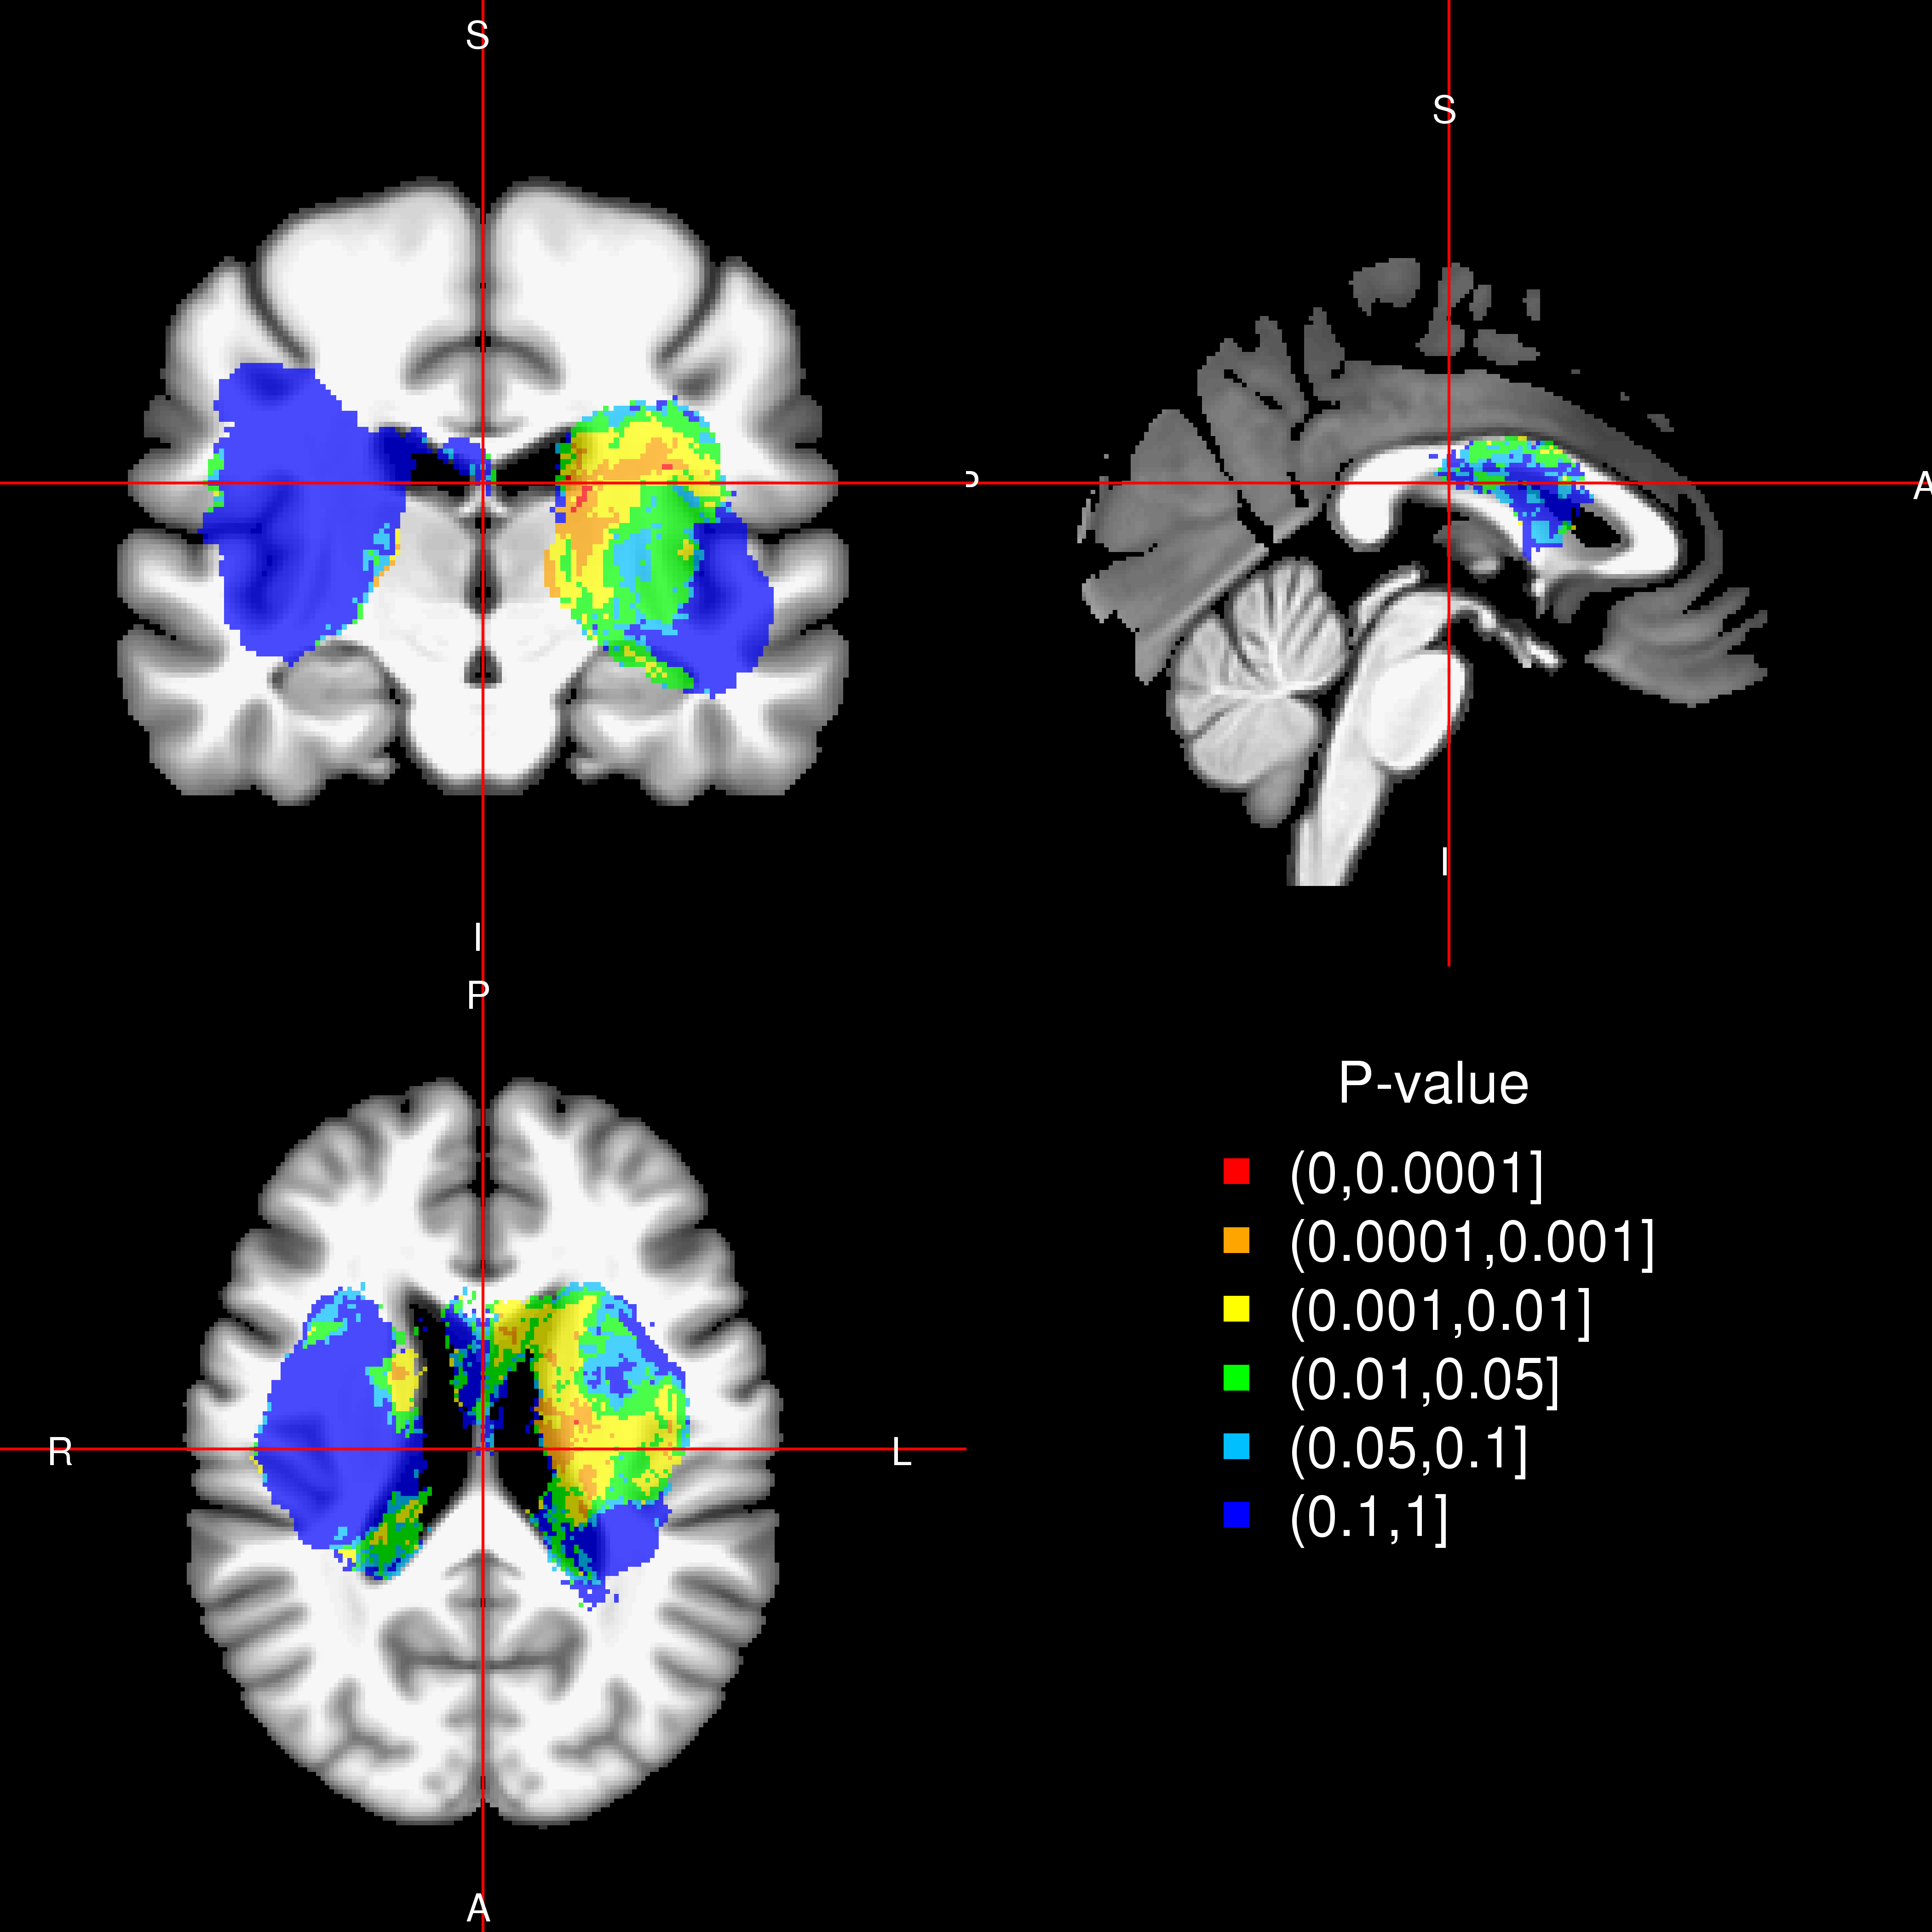
\includegraphics[width=.31\textwidth]{Regression_Map_heatcol6_t1.png}
 } 
  
  \caption{P-value maps for the $6$ models, with NIHSS score as functional outcome. Colors correspond to p-values $.1-1$ (dark blue), $.1-.05$, (light blue), $.05-.01$ (green), $.01-.001$ (yellow),  $.001-.0001$ (orange), and $< .0001$ (red).  We see that in the unadjusted linear model (panel~\protect\subref{mods:m1}) and after adjusting for gender (panel~\protect\subref{mods:m3}) there are voxels with the smallest p-values seem to be near the ventricles.  In models adjusting for age (panel~\protect\subref{mods:m2}), or total baseline ICH volume (panel~\protect\subref{mods:m4}), or both (panel~\protect\subref{mods:m5}), the p-value relating to NIHSS scores appear higher (more bluish).  Also, we see the Wilcoxon rank-sum test have smaller p-values for the same area compared to the unadjusted linear model (panel~\protect\subref{mods:m6}). Slices are presented at the middle of the template.  }
  \label{f:mods}
\end{figure}




\begin{figure}[H]
\centering
  \hfill
  \subfloat[HPR for NIHSS score; voxels with p-values $< .0100$ ]{
 \label{pvals:nihss}
 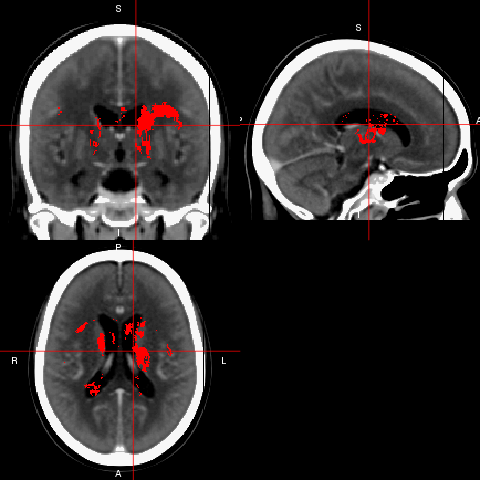
\includegraphics[width=.48\textwidth]{Top_19047_pvalues.png}
 }
  \hfill
  \subfloat[HPR for GCS score; voxels with the lowest $1000$ p-values]{
 \label{pvals:gcs}
 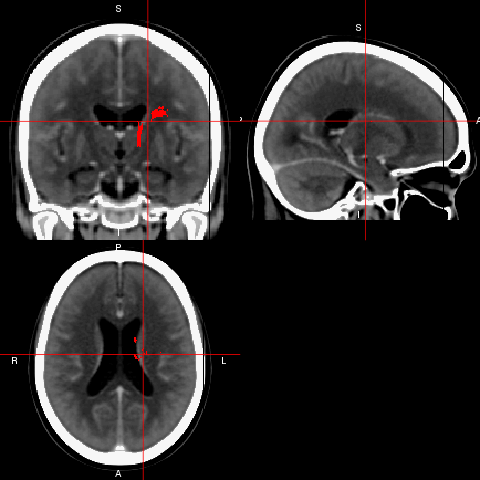
\includegraphics[width=.48\textwidth]{GCS_Top_1000_pvalues.png}
 } 
 \newline
  \hfill
  \subfloat[Relationship of NIHSS score and HPR coverage for HPR in \protect\subref{pvals:nihss}]{
 \label{pvals:regnihss}
 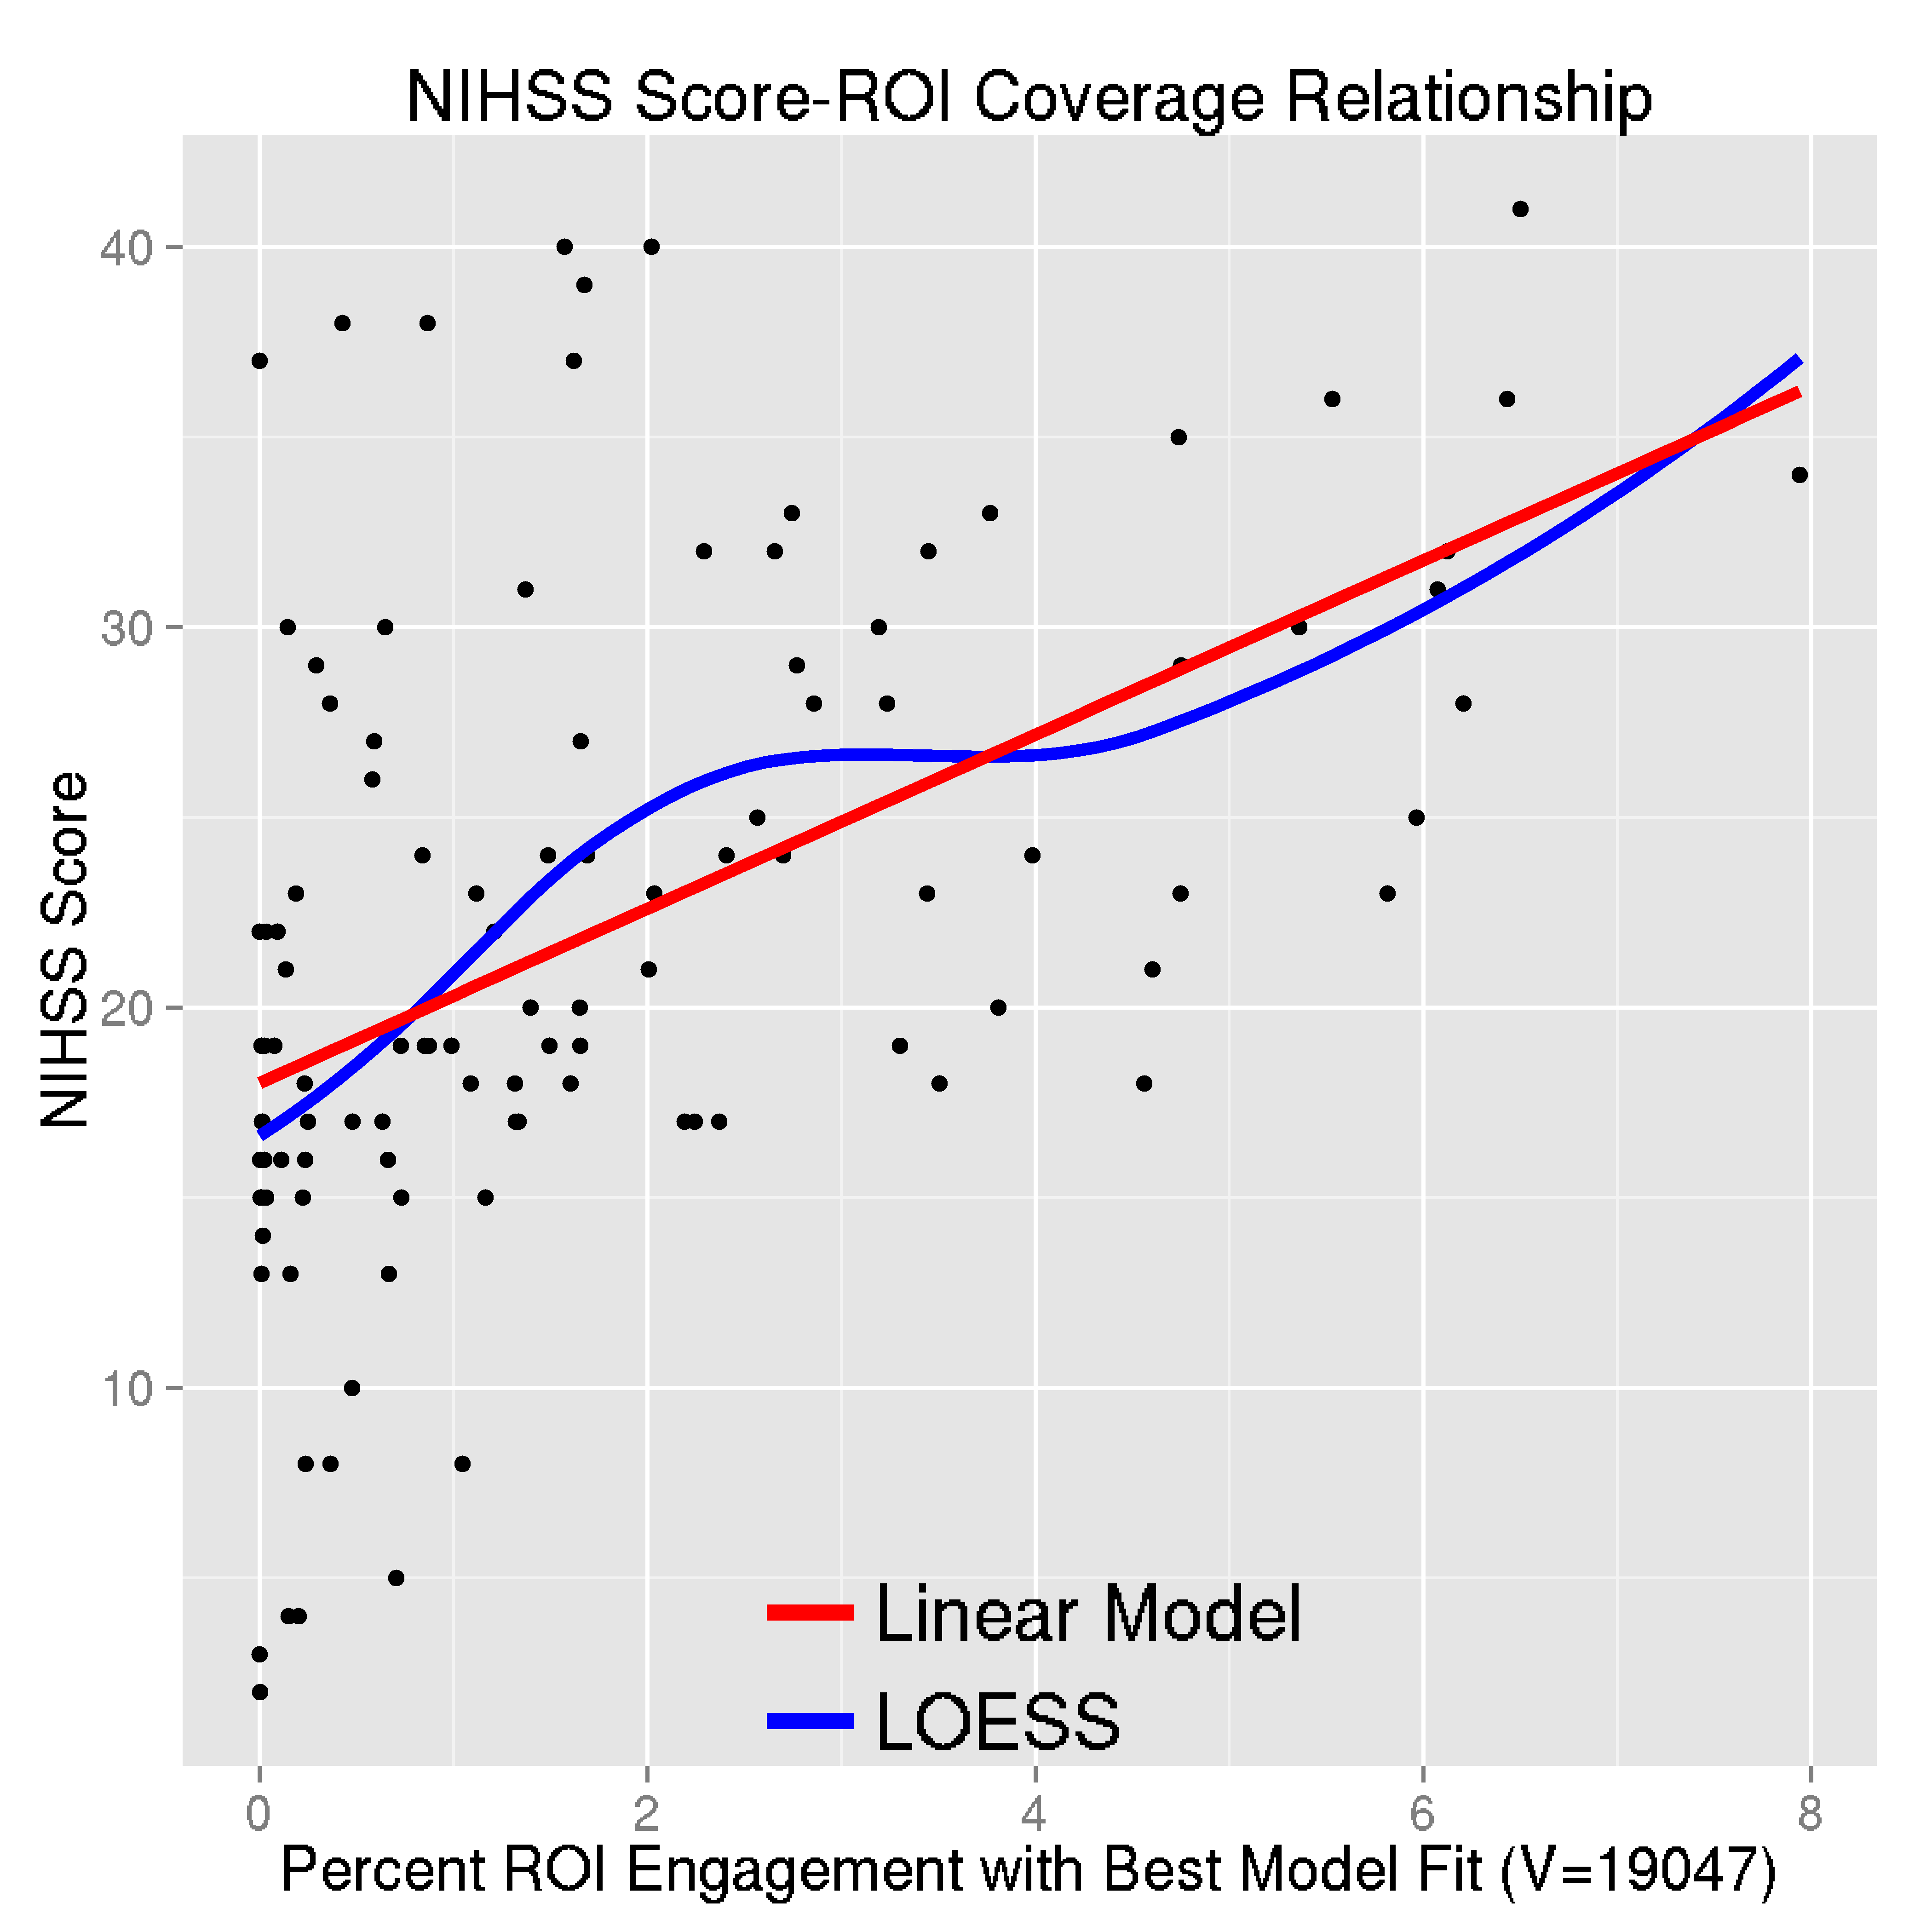
\includegraphics[width=.48\textwidth]{Regress_ROI_NIHSS_Best_Model.png}
 }
  \hfill
  \subfloat[Relationship of GCS score and HPR coverage for HPR in \protect\subref{pvals:gcs}]{
 \label{pvals:reggcs}
 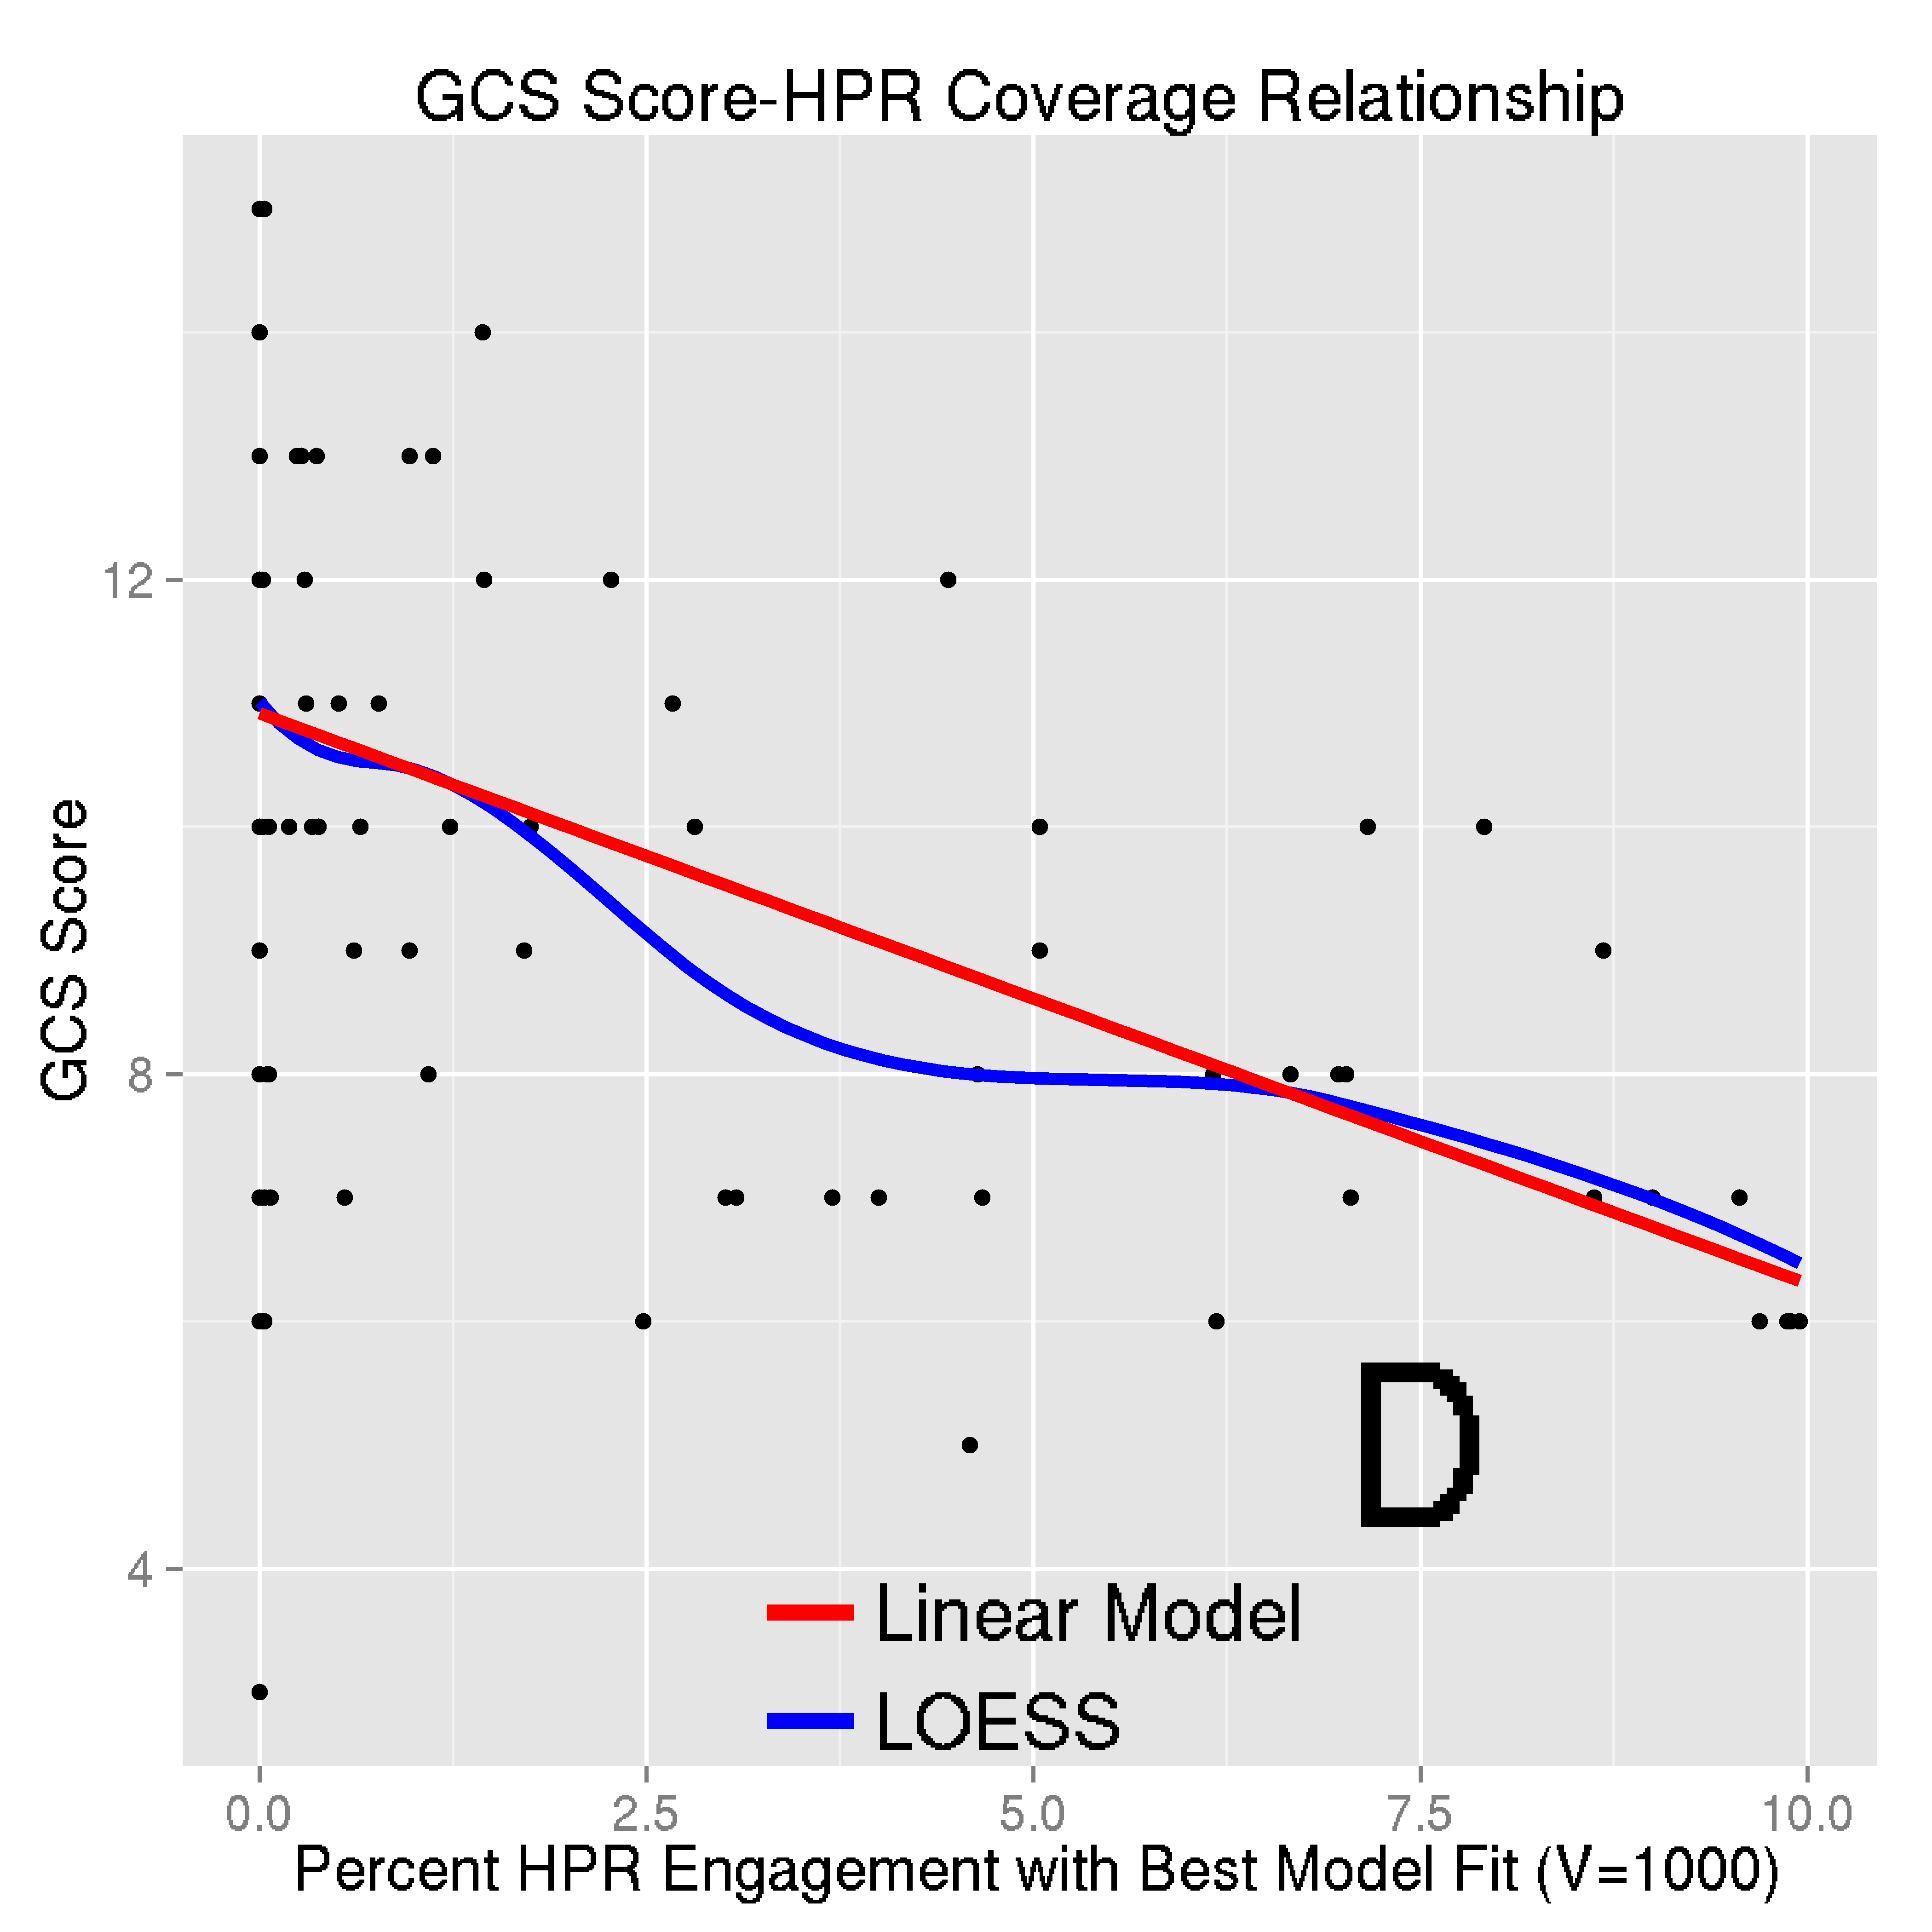
\includegraphics[width=.48\textwidth]{Regress_ROI_GCS_Best_Model.png}
 } 
 \newline 
  
  \caption{Highest Predictive Region (HPR) Analysis.  Panels~\protect\subref{pvals:nihss} and~\protect\subref{pvals:gcs} correspond to the HPR for the top-performing model for NIHSS and GCS scores, respectively.  The HPR in panel~\protect\subref{pvals:nihss} represents a p-value threshold of $.0100$ for the voxel-wise ICH on NIHSS score regressions, which includes $19047$ voxels. The HPR in panel~\protect\subref{pvals:gcs} represents $1000$ with the lowest p-values for the voxel-wise ICH on GCS score regressions, corresponding to a p-value threshold of $.0002$.
    Panels~\protect\subref{pvals:regnihss} and~\protect\subref{pvals:reggcs} display the relationship of the HPR coverage to the functional score.  The red line represents a linear fit (without adjustment of other covariates) of the HPR coverage and functional score and the blue line represents a LOESS fit.  We see that the larger the HPR coverage the higher (more severe stroke) NIHSS score and the lower (deeper unconsciousness) the GCS score.  
}
  \label{f:roi}
\end{figure}





% \begin{figure}[htbp]
% \centering
%  \subfloat[$\mathcal{M}_1:$ unadjusted]{
%  \label{mods:m1}
%  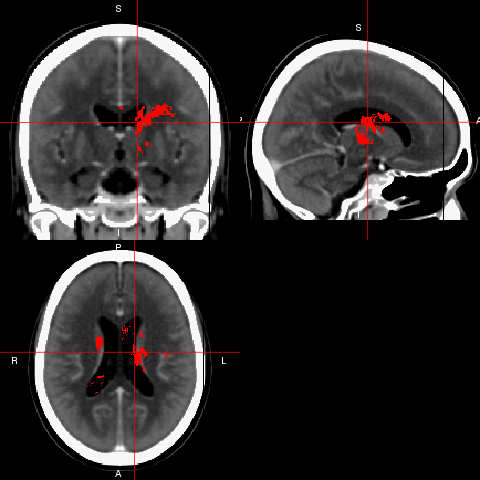
\includegraphics[width=.31\textwidth]{Regression_Map_FDR_red_1_centered.png}
%  }
%   \hfill
%   \subfloat[$\mathcal{M}_3:$ adjusted for Gender]{
%  \label{mods:m3}
%  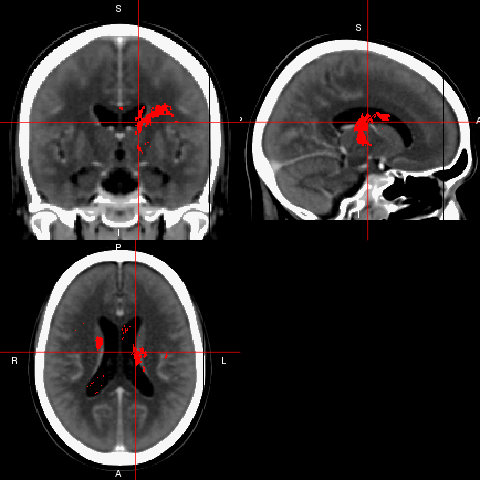
\includegraphics[width=.31\textwidth]{Regression_Map_FDR_red_3_centered.png}
%  }
%   \subfloat[$\mathcal{M}_6$: voxel-wise Wilcoxon rank-sum test for NIHSS distribution]{
%  \label{mods:m6}
%  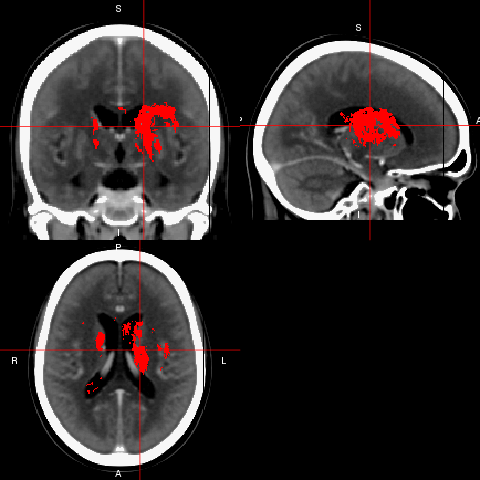
\includegraphics[width=.31\textwidth]{Regression_Map_FDR_red_6_centered.png}
%  } 
  
%   \caption{FDR-corrected significant ($α ≤ .05$) p-values for the $3$ models.  }
%   \label{f:mods}
% \end{figure}



%\begin{tabular}{lll}
%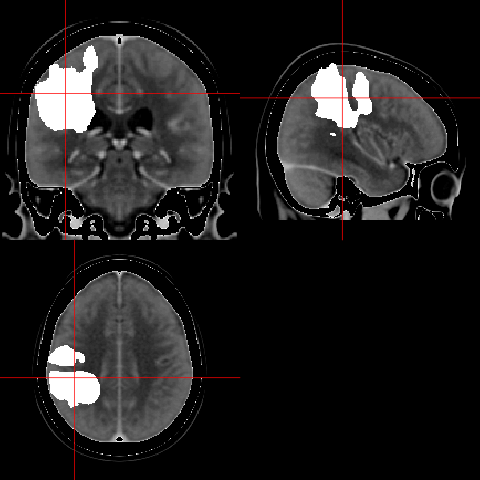
\includegraphics[scale=.3]{roi_spm_100-362_20100126_1926_CT_2_CT_ROUTINE.png} & 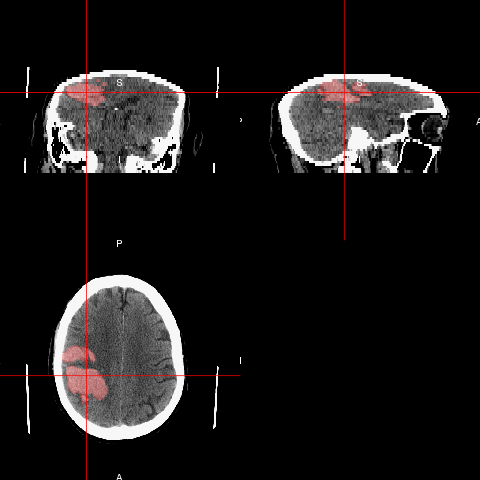
\includegraphics[scale=.3]{native_100-362_20100126_1926_CT_2_CT_ROUTINE.png} & 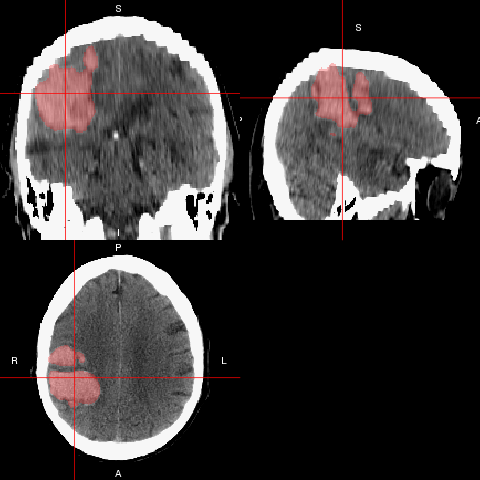
\includegraphics[scale=.3]{raw_spm_100-362_20100126_1926_CT_2_CT_ROUTINE.png}
%\end{tabular}


% \caption{Histograms of sex, age (in years), sex, and NIHSS scores (in years) for the patients in the study.}\label{fig:histdem}
% \end{figure}

\newpage
\section{Supplemental Material}


\begin{figure}[H]
\centering
 \subfloat[$\mathcal{M}_1:$ unadjusted]{
 \label{gcsmods:m1}
 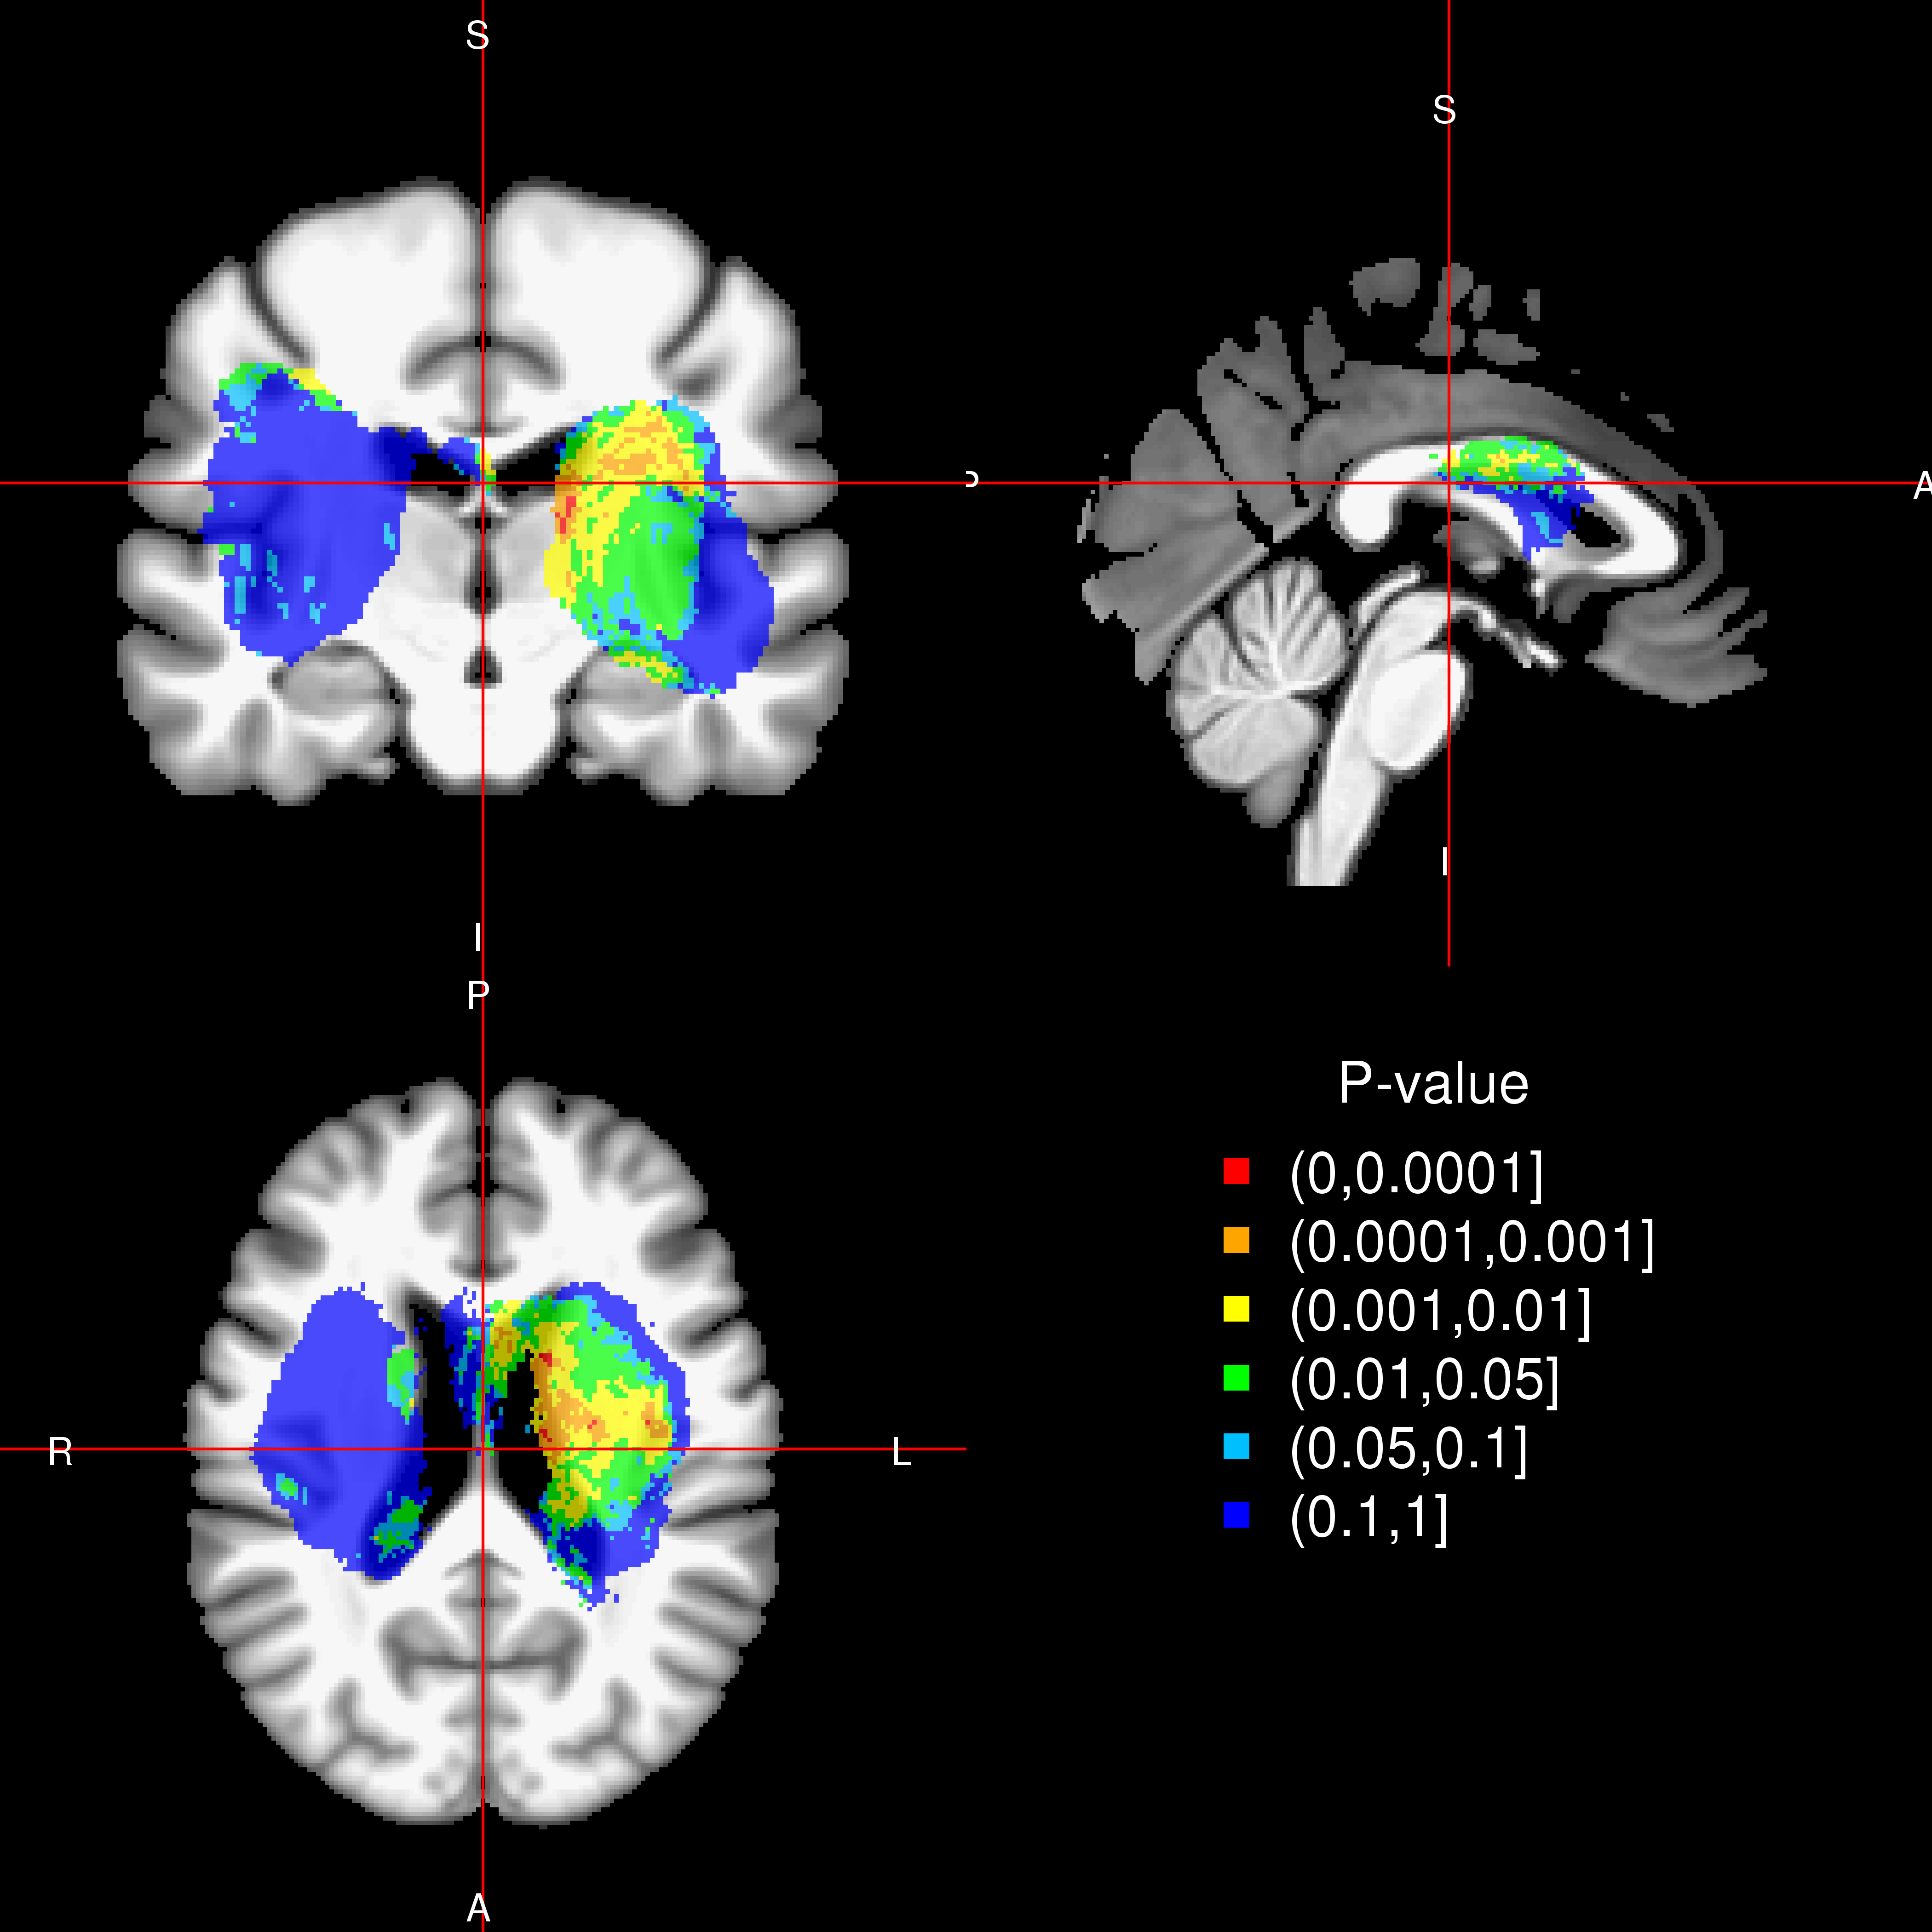
\includegraphics[width=.31\textwidth]{GCS_Regression_Map_heatcol1_t1.png}
 }
  \hfill
  \subfloat[$\mathcal{M}_2:$ adjusted for Age]{
 \label{gcsmods:m2}
 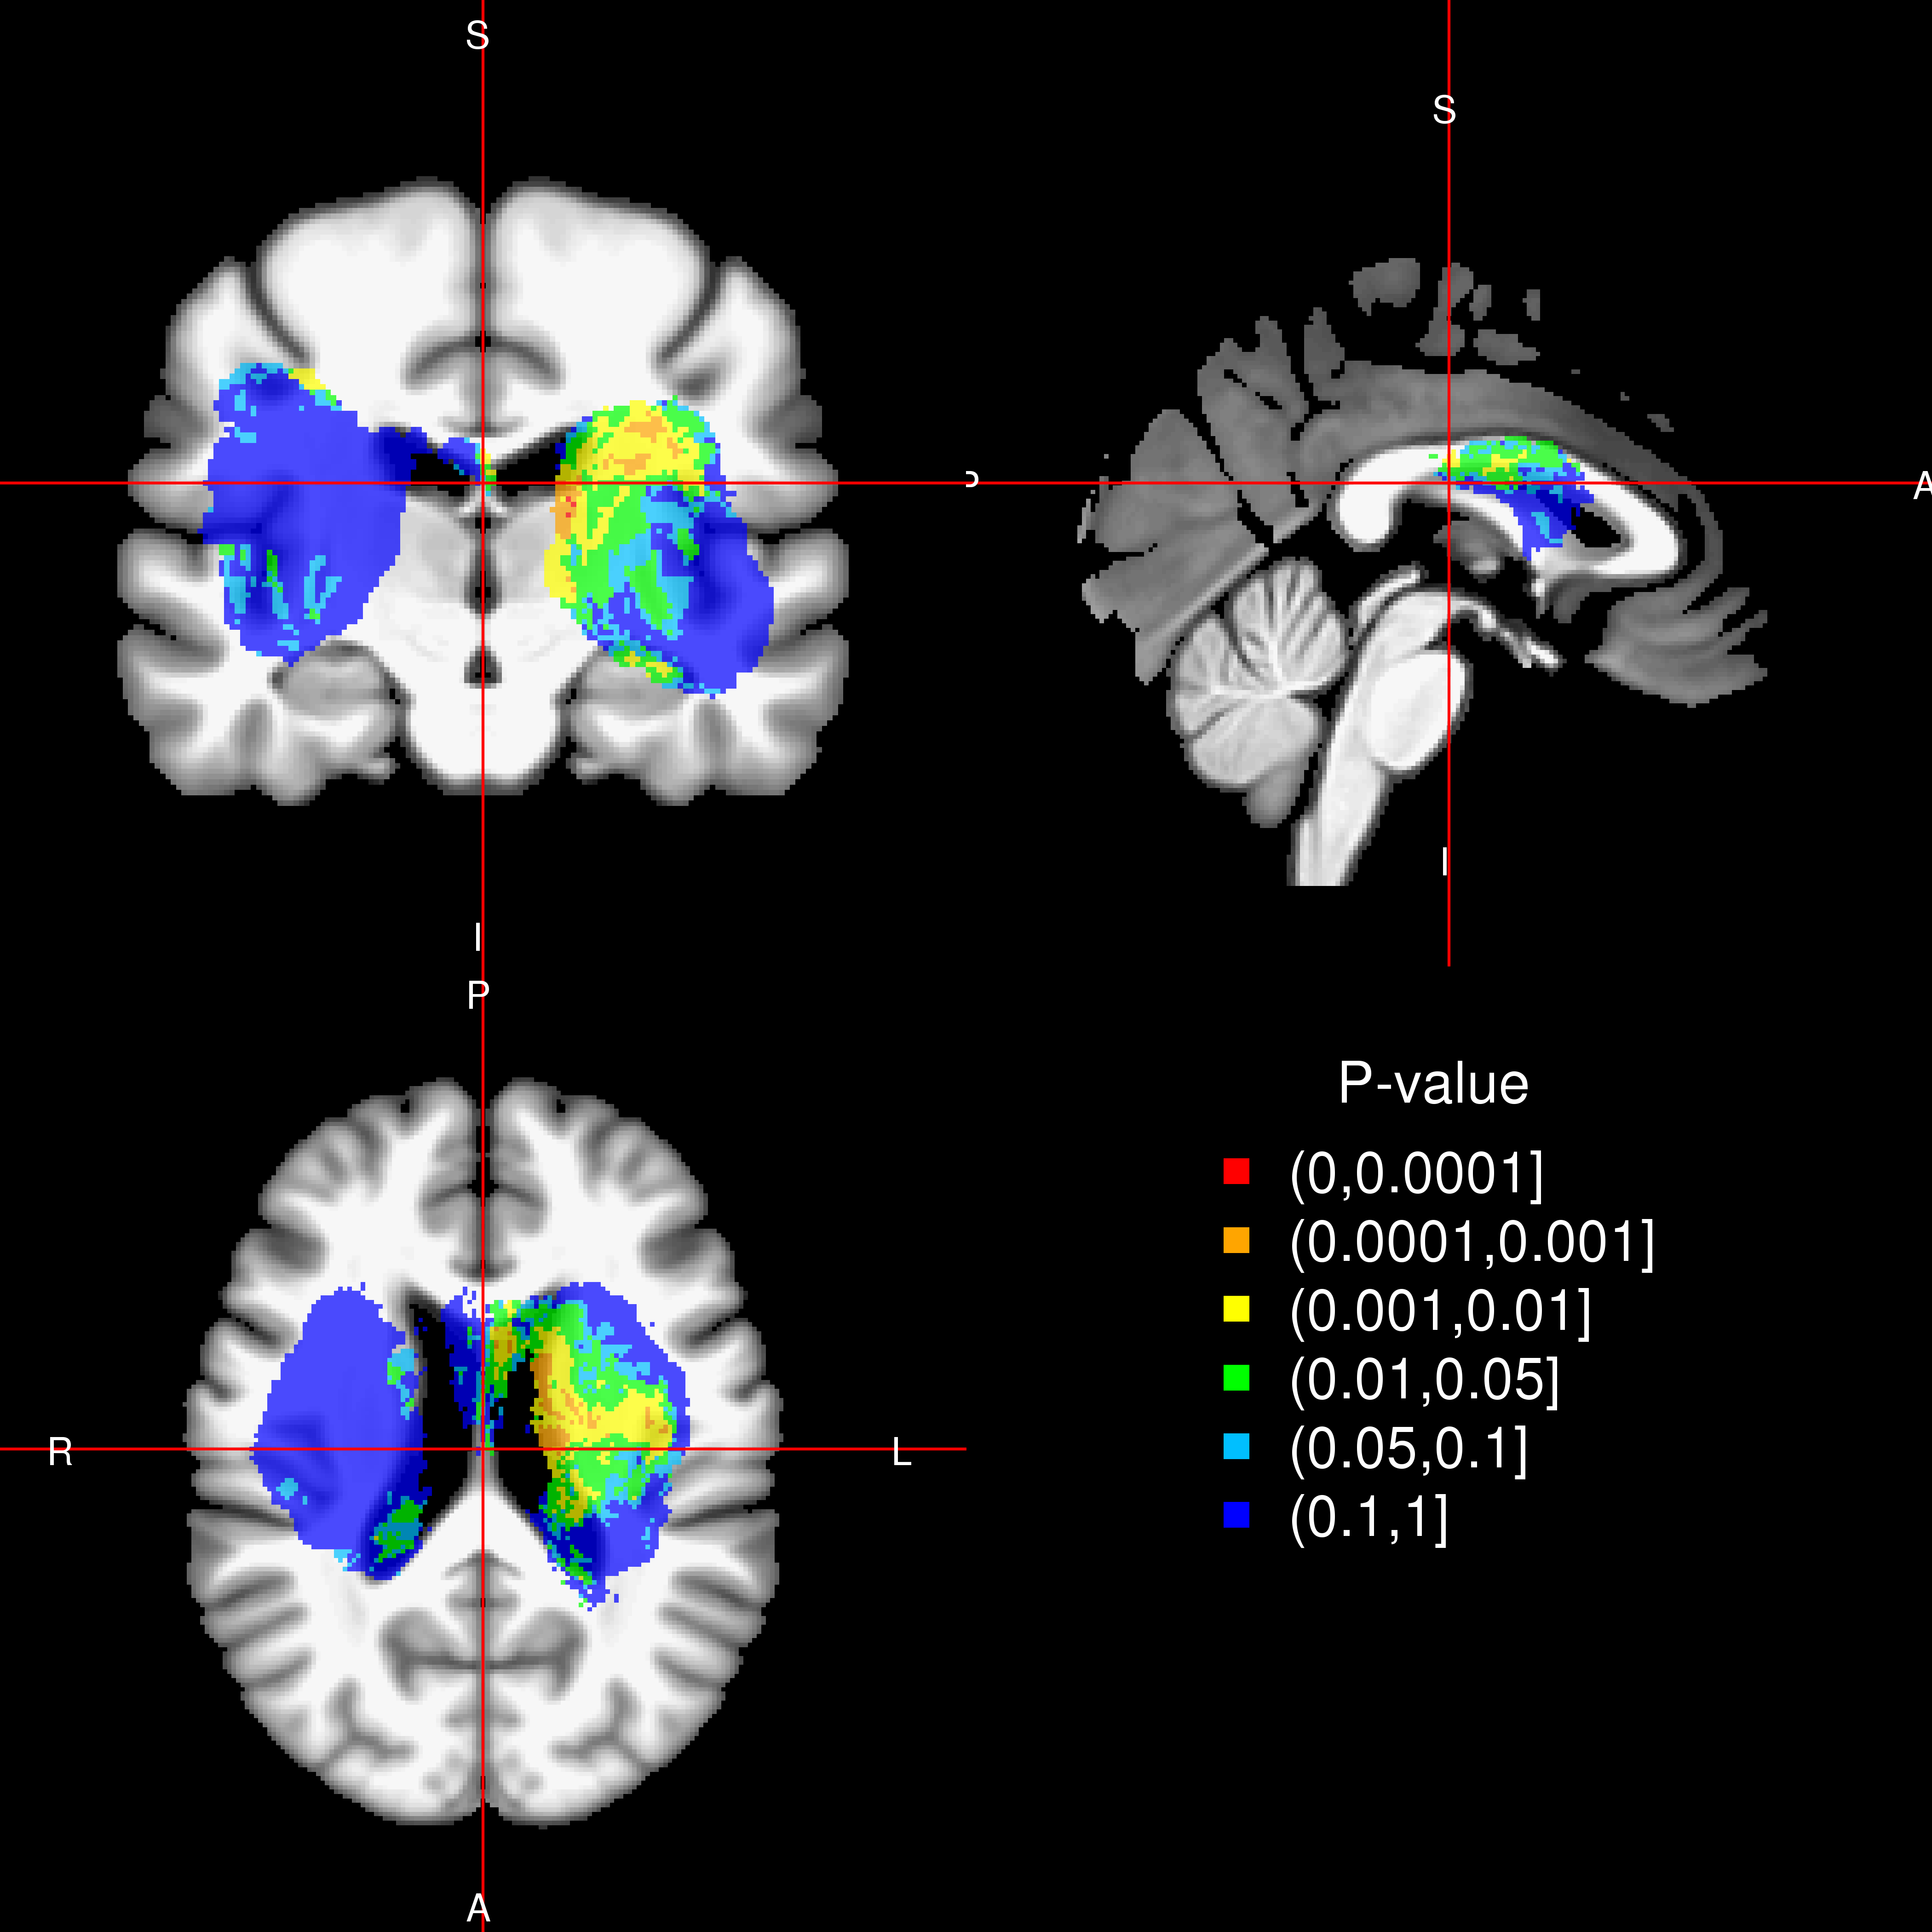
\includegraphics[width=.31\textwidth]{GCS_Regression_Map_heatcol2_t1.png}
 }
  \hfill
  \subfloat[$\mathcal{M}_3:$ adjusted for Gender]{
 \label{gcsmods:m3}
 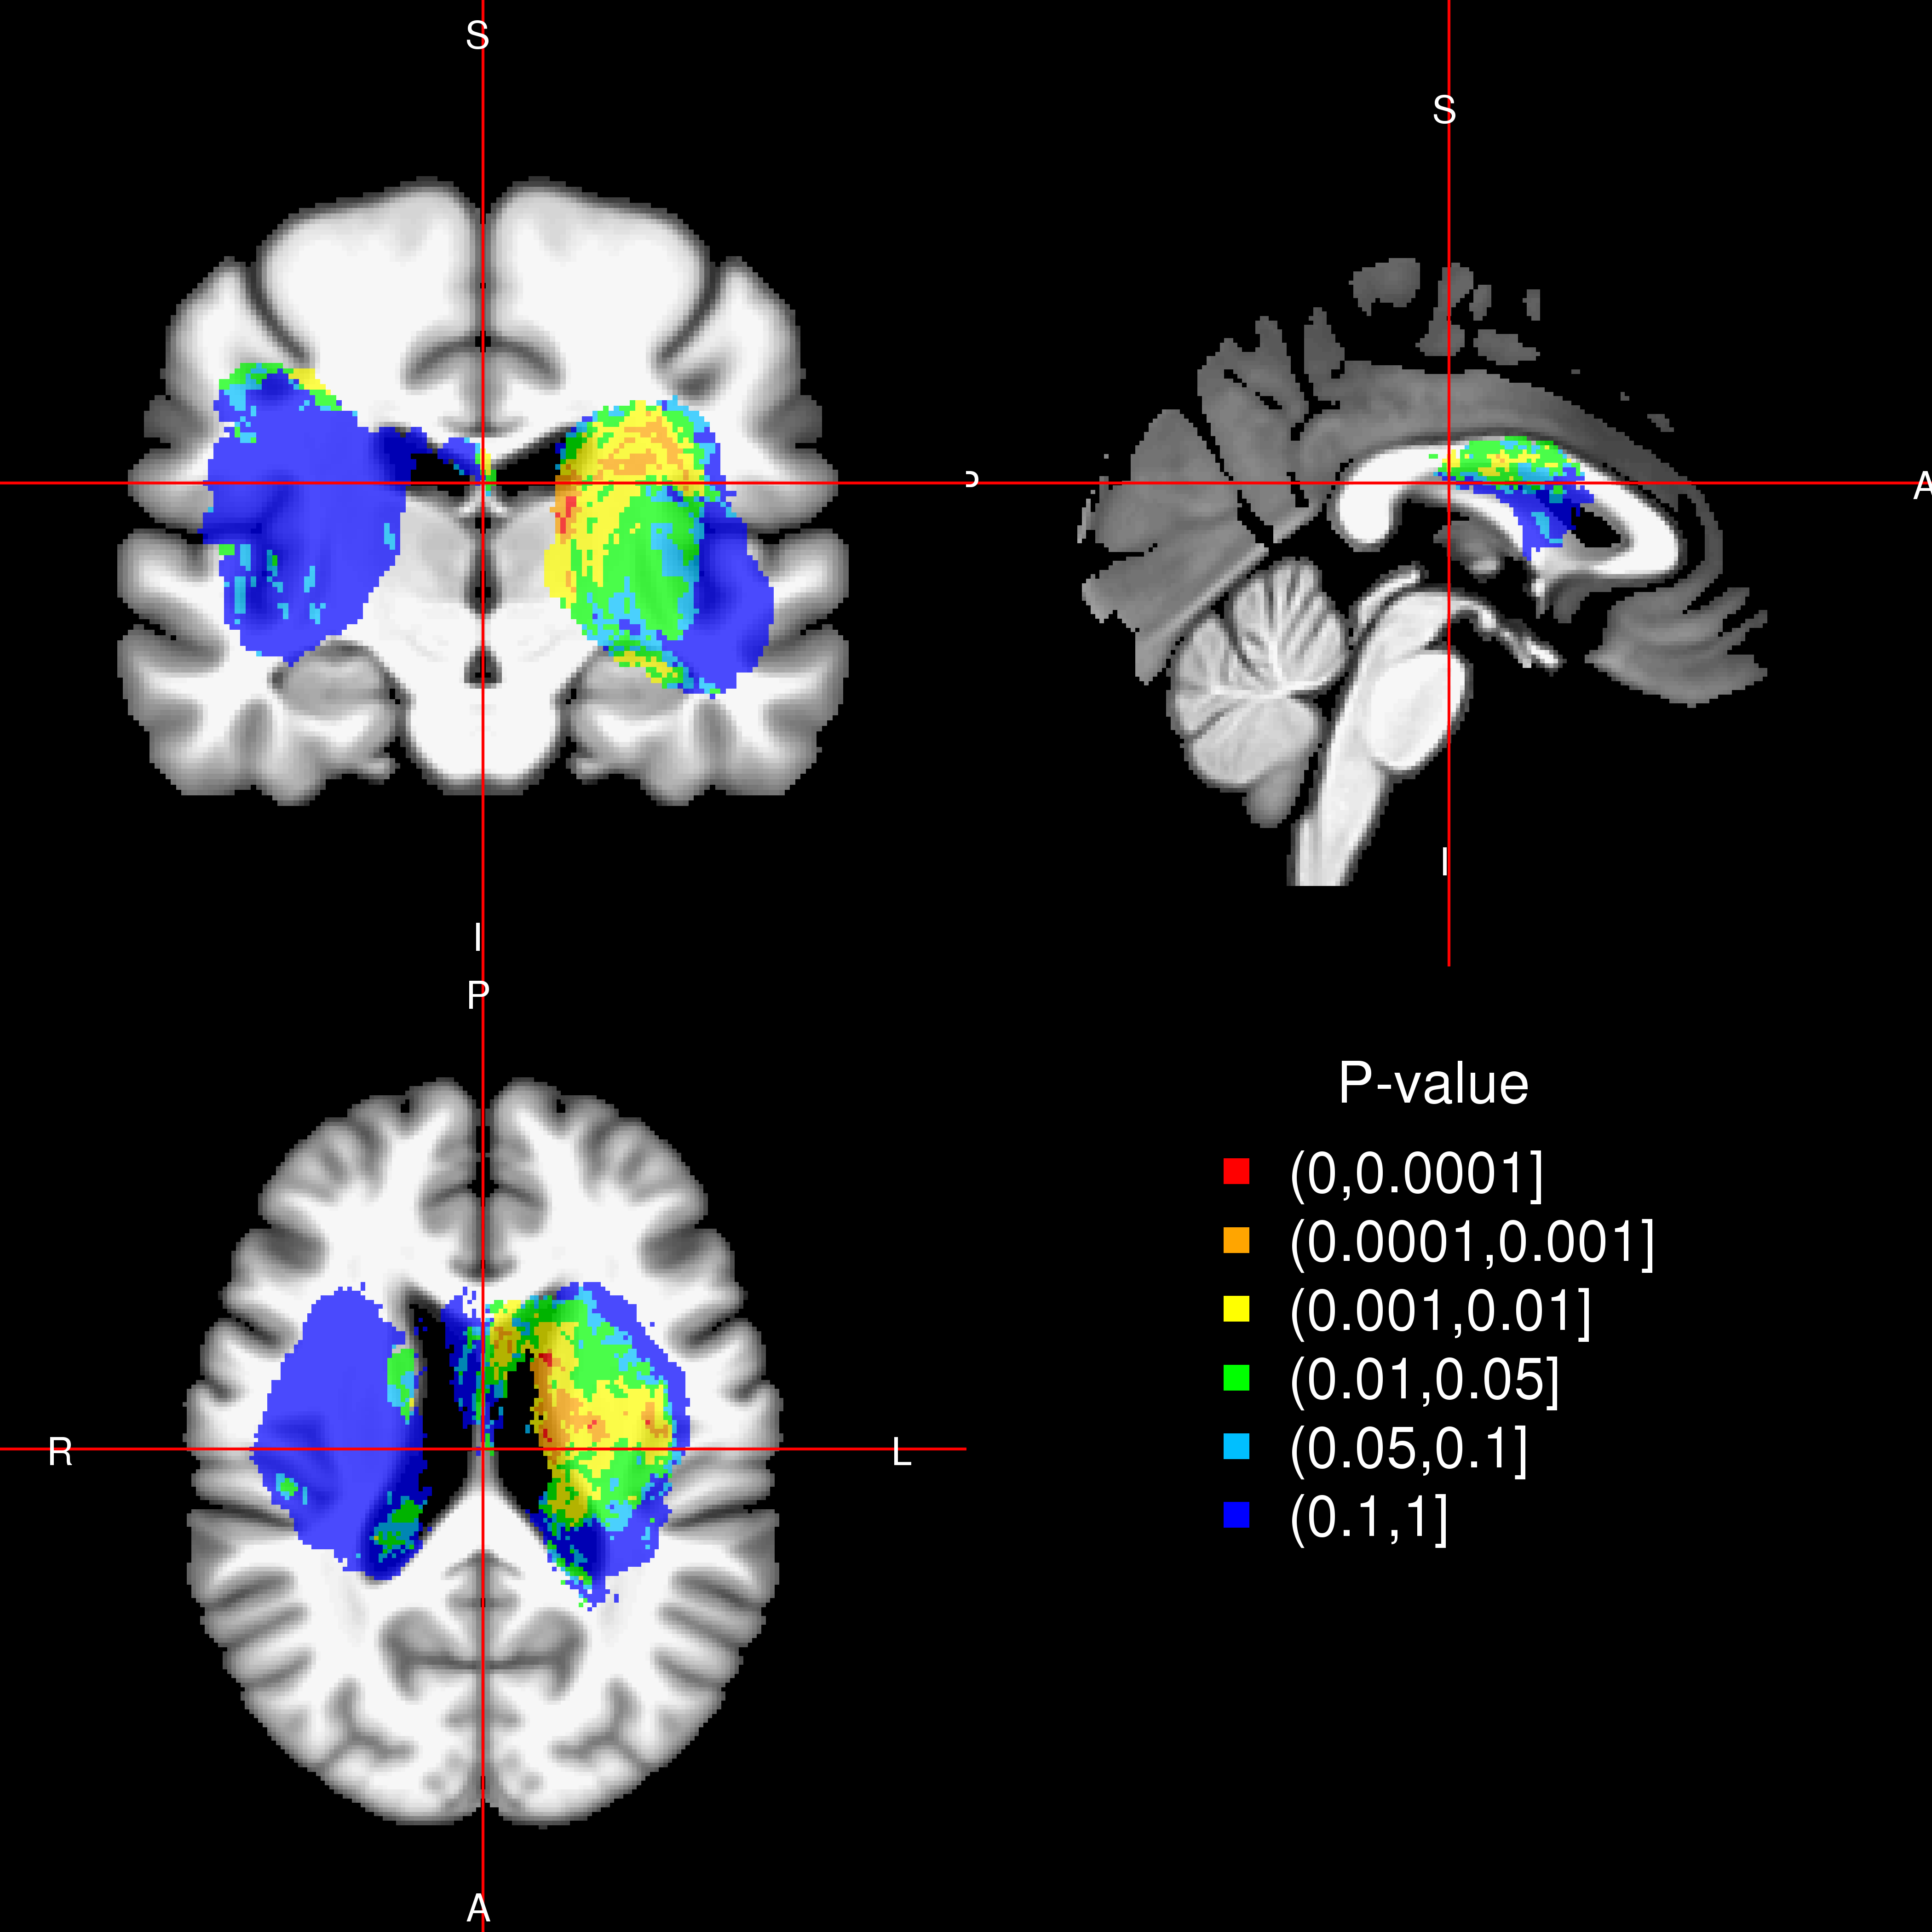
\includegraphics[width=.31\textwidth]{GCS_Regression_Map_heatcol3_t1.png}
 }
\newline
  \subfloat[$\mathcal{M}_4:$ adjusted for total baseline ICH volume]{
 \label{gcsmods:m4}
 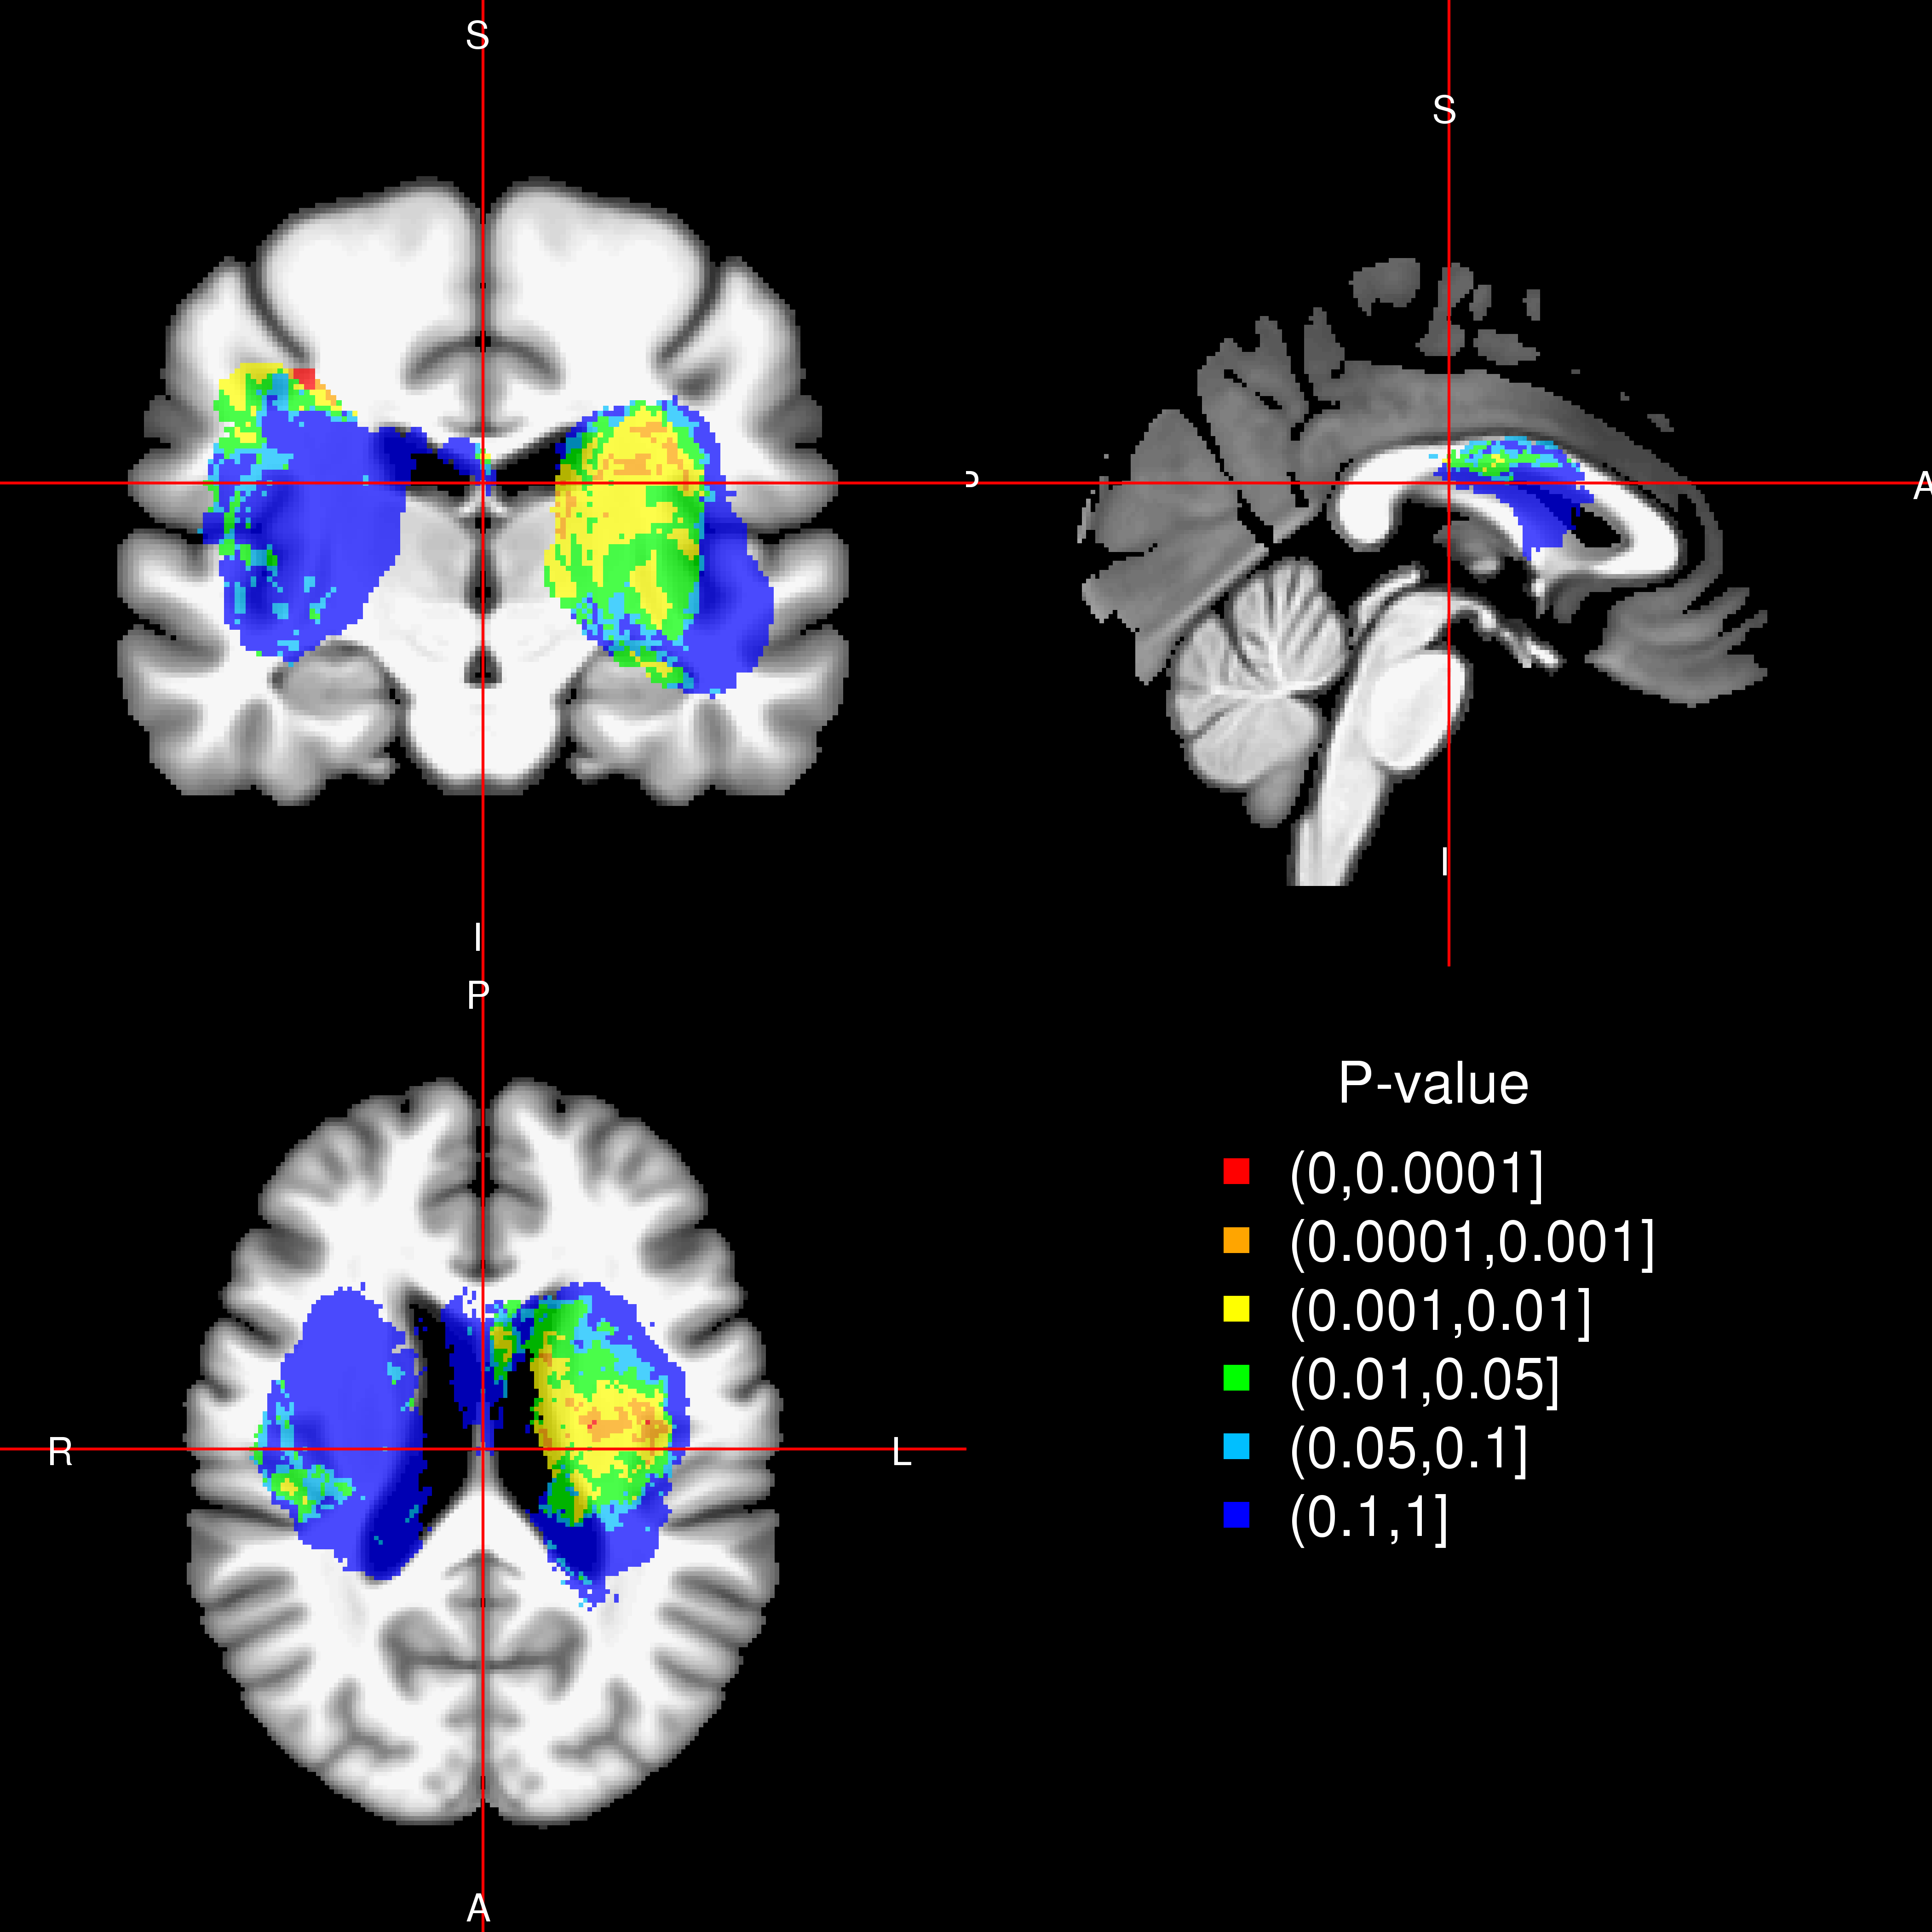
\includegraphics[width=.31\textwidth]{GCS_Regression_Map_heatcol4_t1.png}
 }
  \hfill
  \subfloat[$\mathcal{M}_5:$ adjusted for Age, Gender, total baseline ICH volume ]{
 \label{gcsmods:m5}
 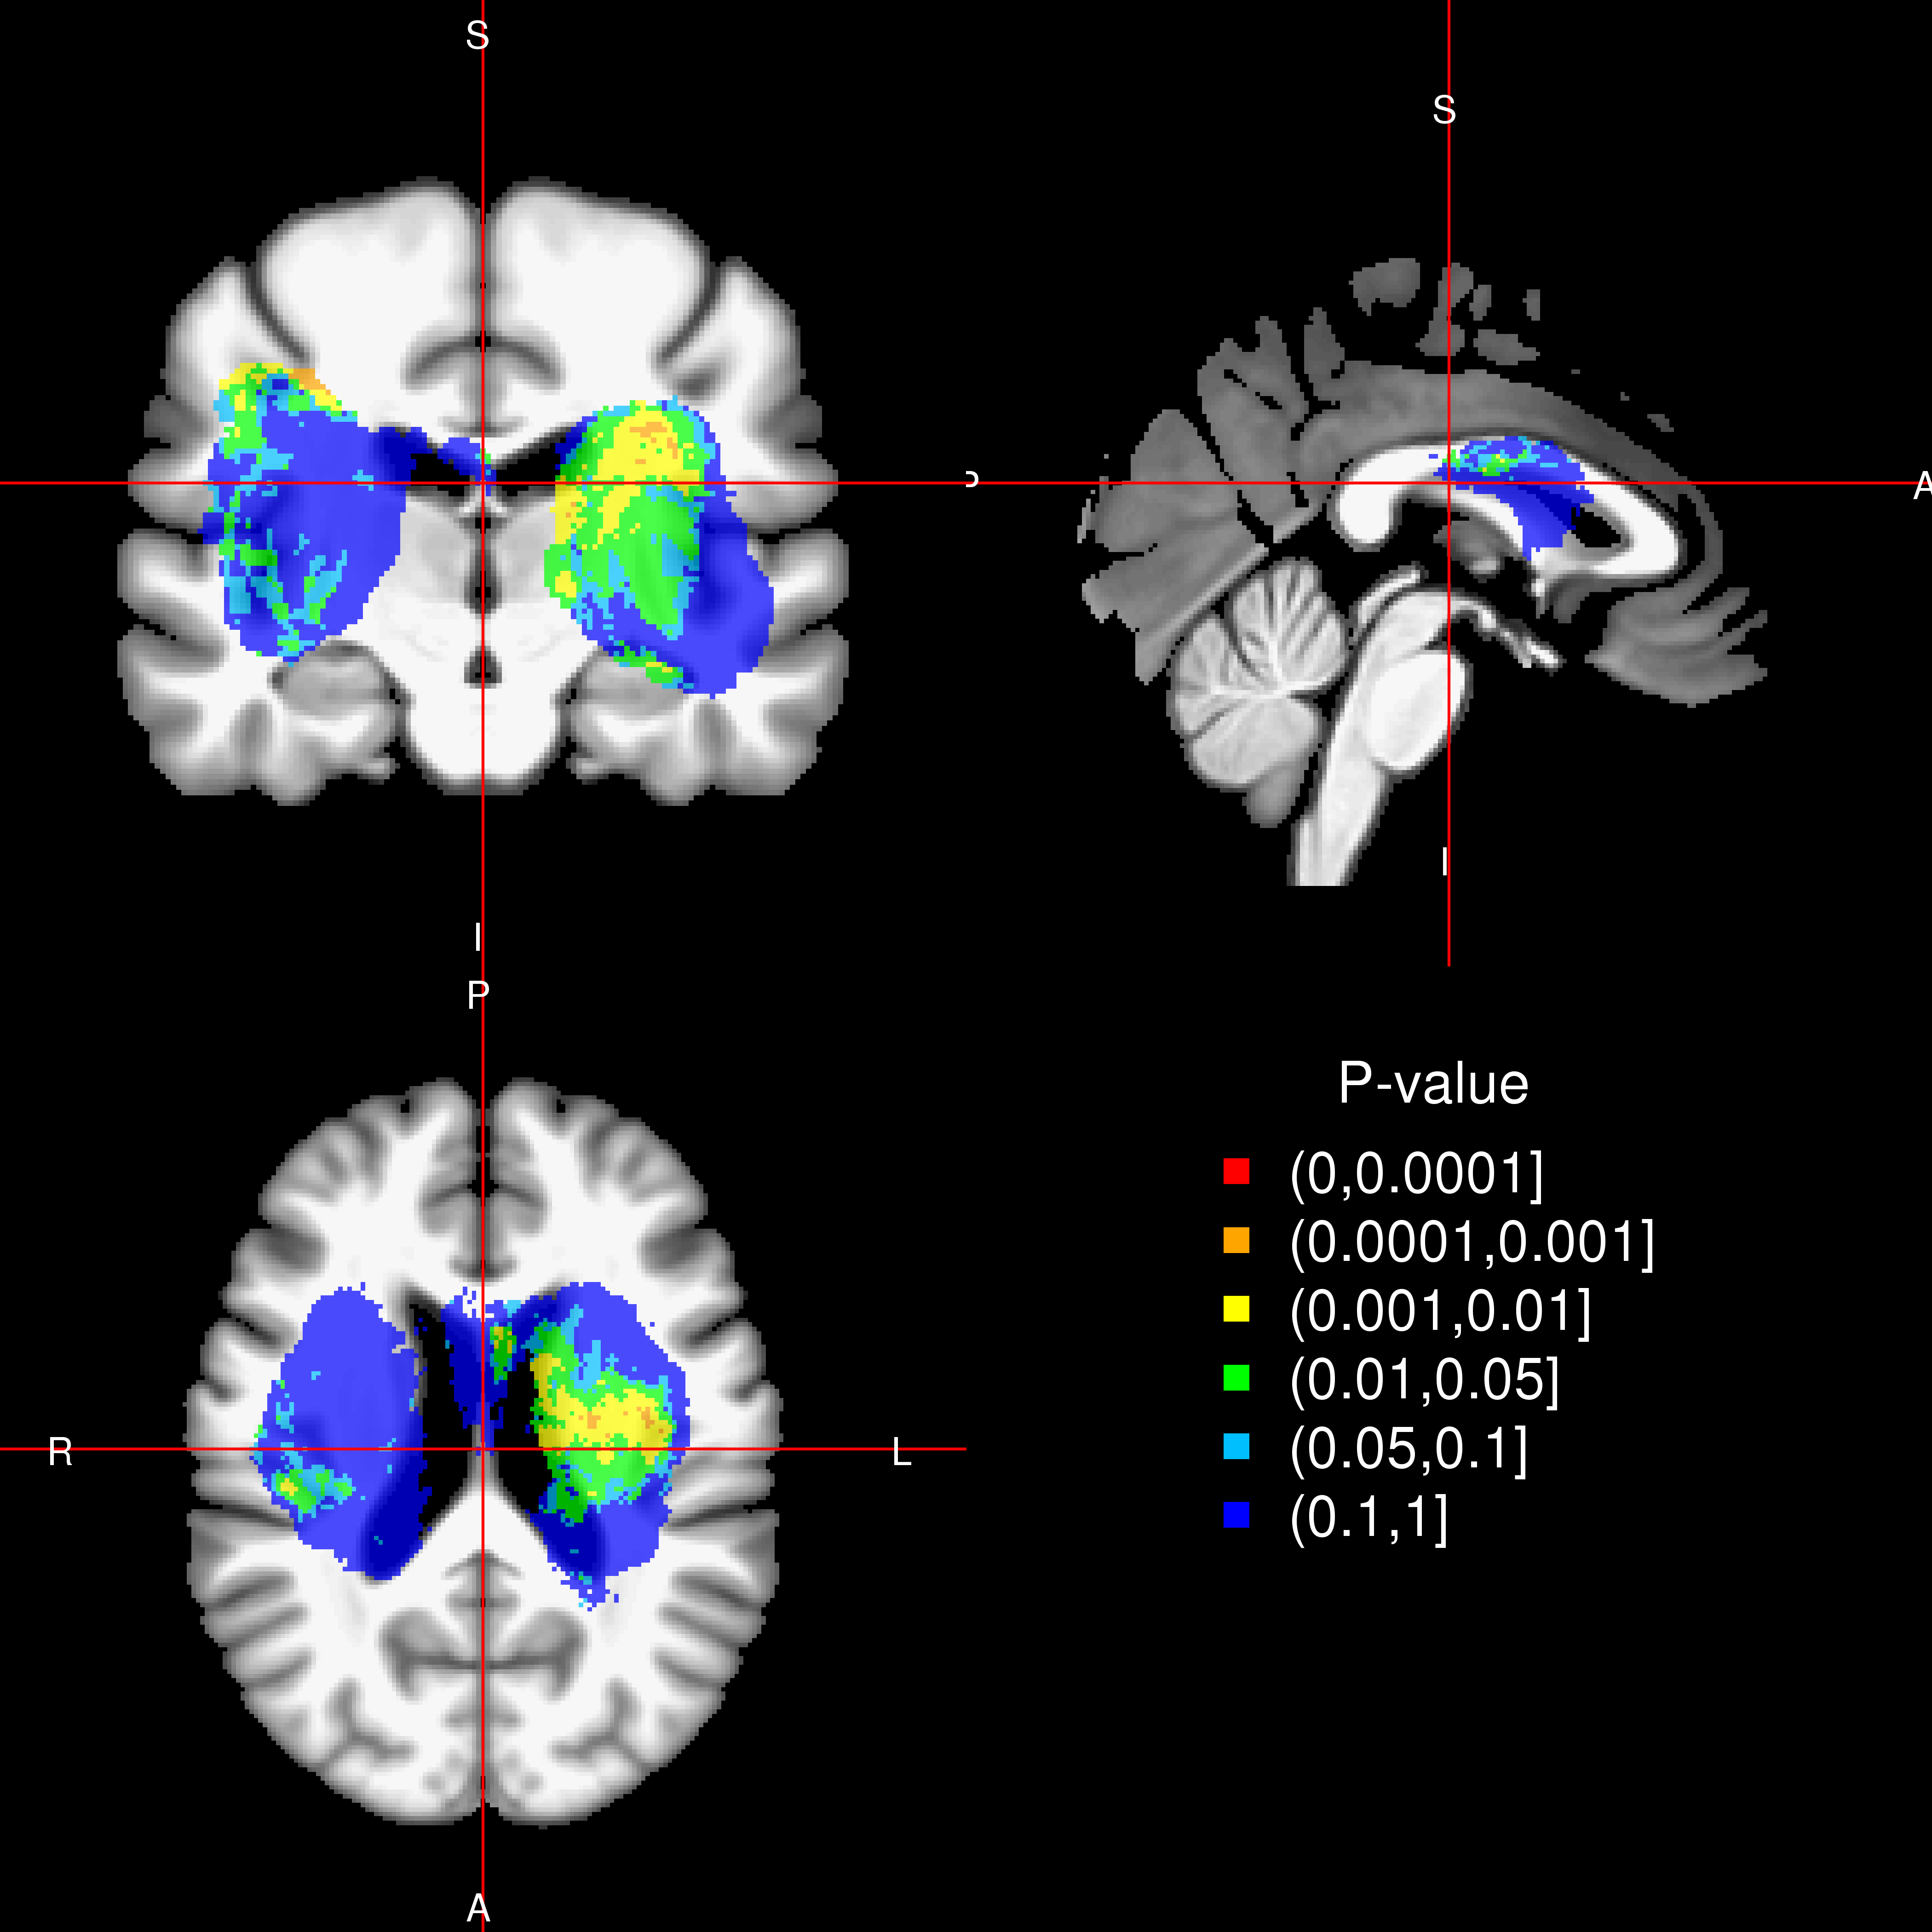
\includegraphics[width=.31\textwidth]{GCS_Regression_Map_heatcol5_t1.png}
 }
  \hfill
  \subfloat[$\mathcal{M}_6$: voxel-wise Wilcoxon rank-sum test for GCS score distribution]{
 \label{gcsmods:m6}
 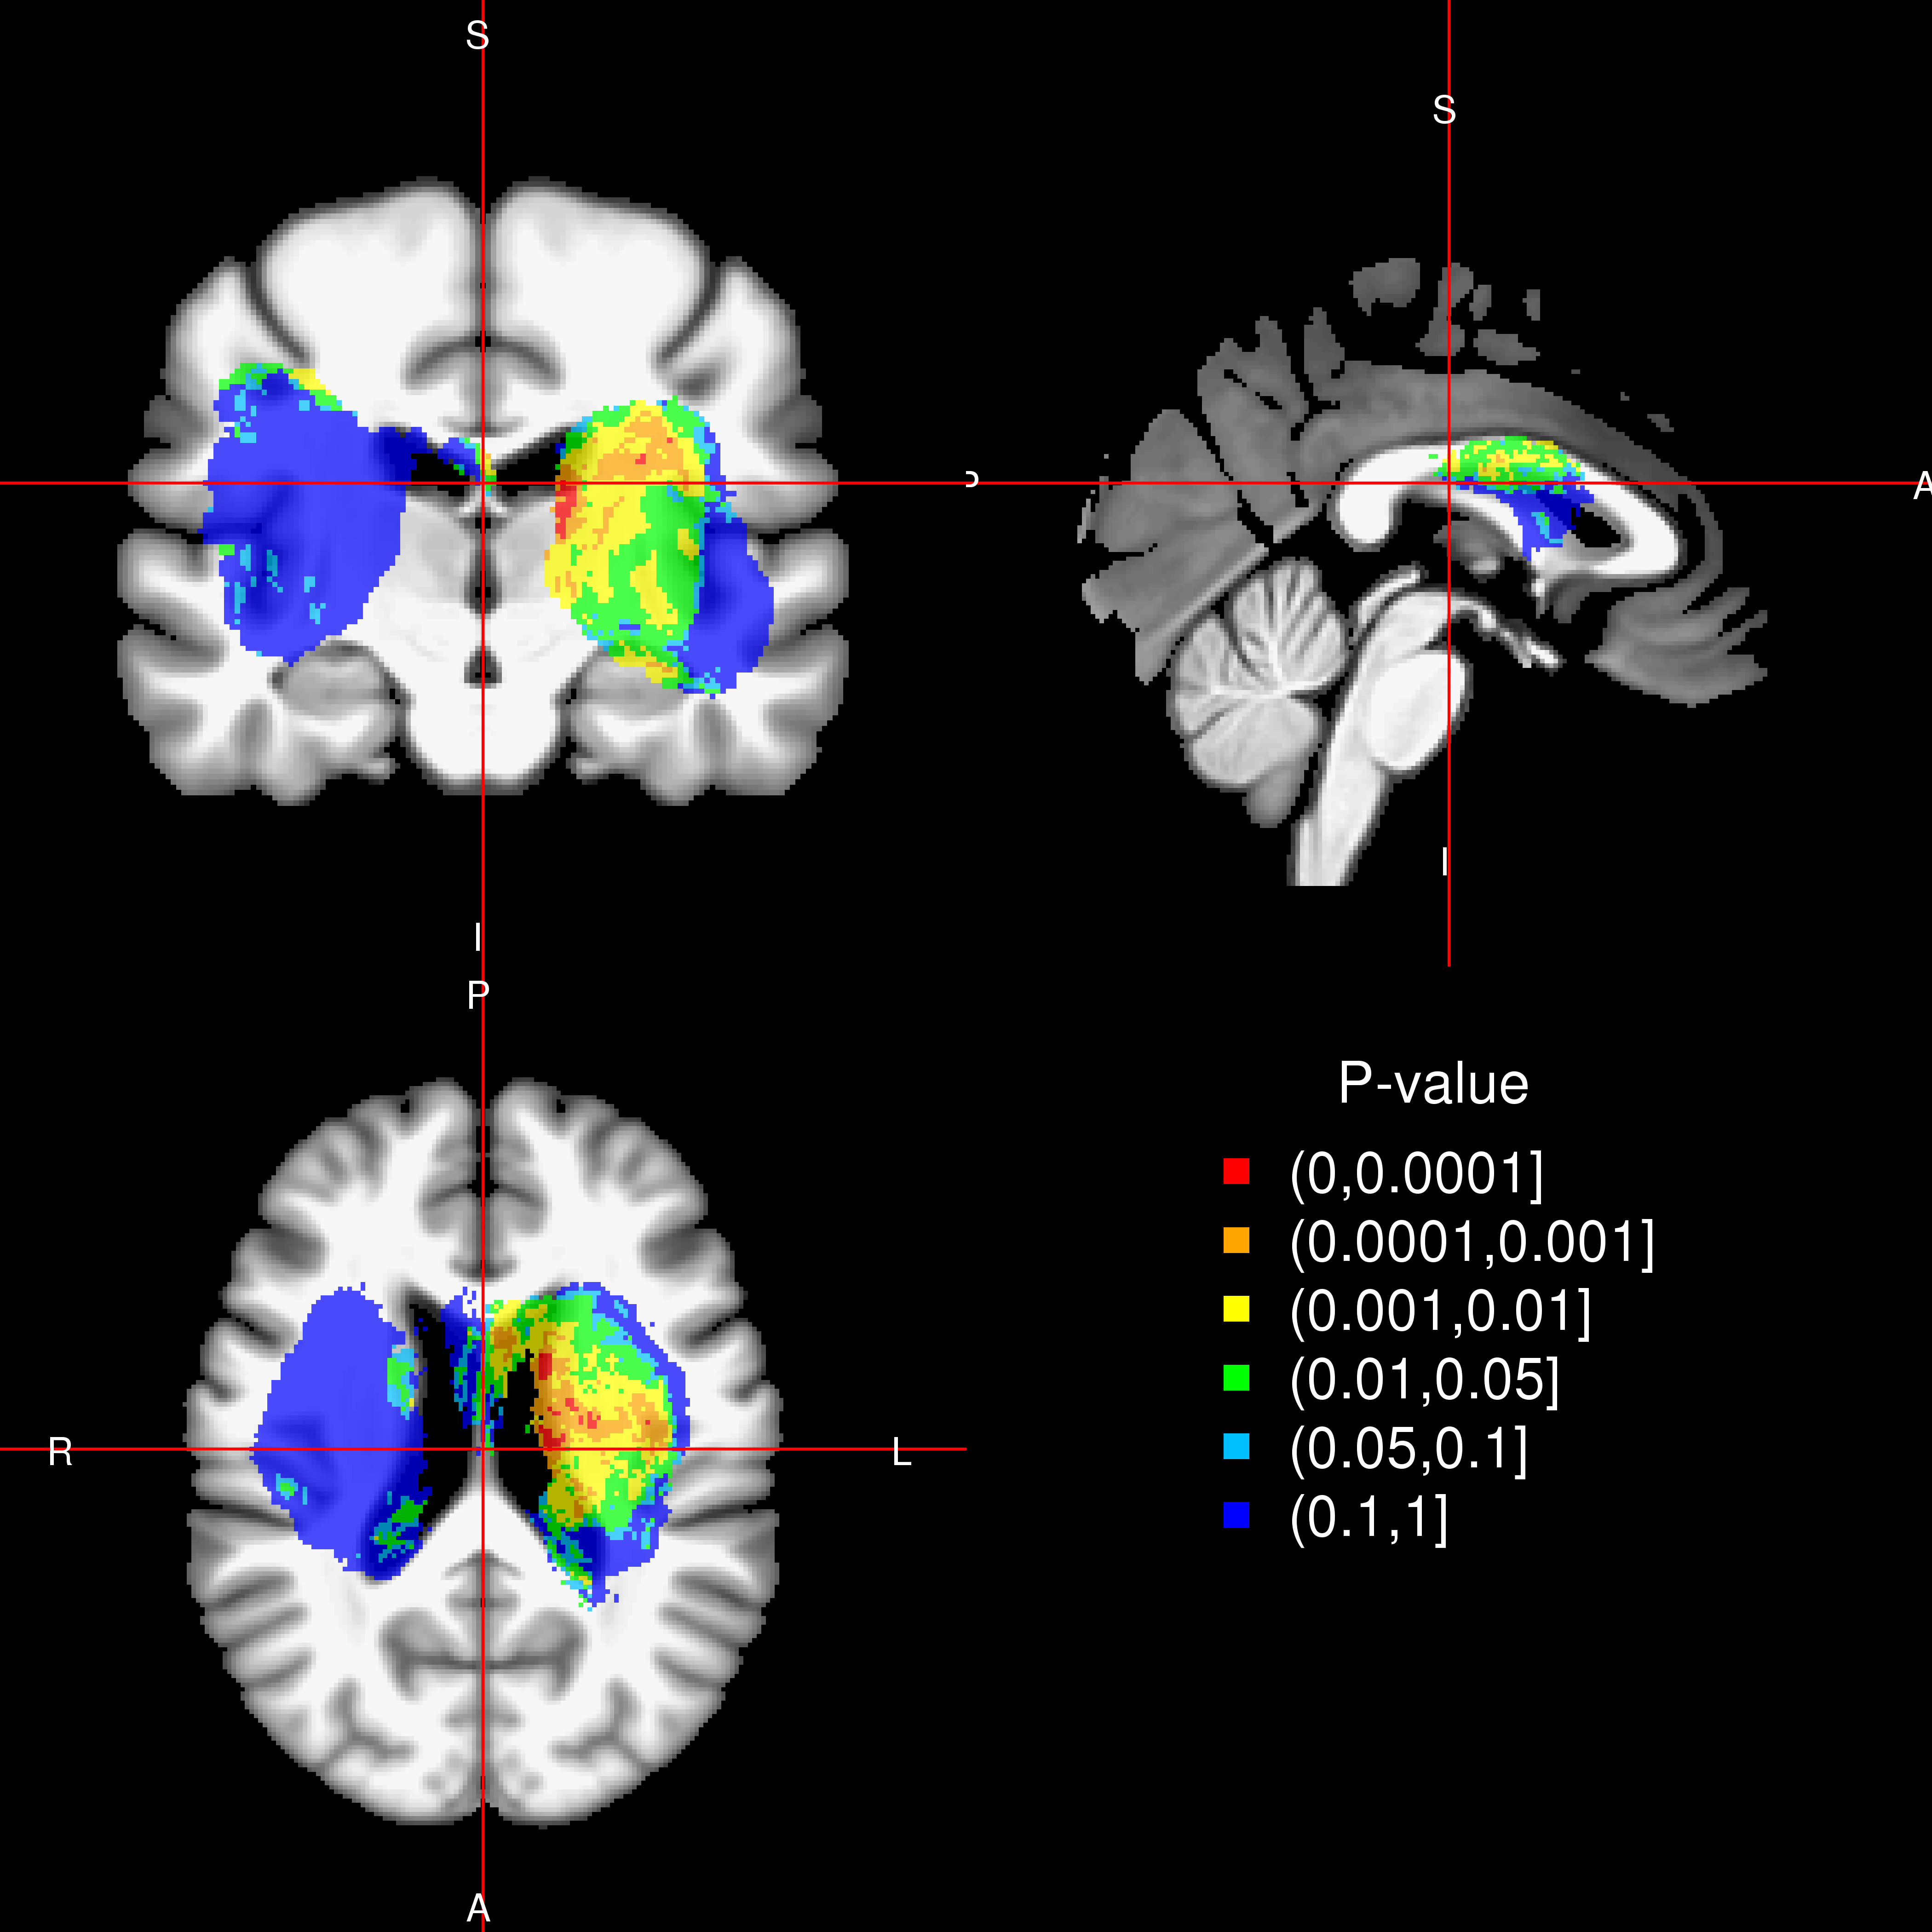
\includegraphics[width=.31\textwidth]{GCS_Regression_Map_heatcol6_t1.png}
 } 
  
  \caption{P-value maps for the $6$ models, with GCS score as functional outcome. Colors correspond to p-values $.1-1$ (dark blue), $.1-.05$, (light blue), $.05-.01$ (green), $.01-.001$ (yellow),  $.001-.0001$ (orange) $< .0001$ (red).  We see that in the unadjusted linear model (panel~\protect\subref{gcsmods:m1}) and after adjusting for gender (panel~\protect\subref{gcsmods:m3}) there are voxels with the smallest p-values seem to be near the ventricles.  In models adjusting for age (panel~\protect\subref{gcsmods:m2}), or total baseline ICH volume (panel~\protect\subref{gcsmods:m4}), or both (panel~\protect\subref{gcsmods:m5}), the p-value relating to GCS scores appear higher (more bluish).  Also, we see the Wilcoxon rank-sum test have smaller p-values for the same area compared to the unadjusted linear model (panel~\protect\subref{gcsmods:m6}). Slices are presented at the middle of the template.  }
  \label{f:gcsmods}
\end{figure}


\end{document}

ADD:
Matching of patients
Results from threshold
More introduction

